\documentclass[11pt]{article}

%
% Dokument Layout
%
\usepackage[lmargin = {2.7cm},  % linker Rand
            rmargin = {3.5cm},  % rechter Rand
            tmargin = {2.2cm},  % oberer Rand
            bmargin = {2.2cm}   % unterer Rand
           ]{geometry}
\marginparsep = 0.6cm           % Abstand zwischen Body und rechter Rand


%
% Pakete
%
\usepackage{attrib}
\usepackage[german,ngerman]{babel}
\usepackage{booktabs}
\usepackage{color}
\usepackage[german=quotes]{csquotes}
\usepackage{float}
\usepackage{graphics}
\usepackage[demo]{graphicx}
\usepackage[T1]{fontenc}
\usepackage{hyperref}
\usepackage[utf8]{inputenc}
\usepackage{lmodern}
\usepackage{listings}
\usepackage{nameref}
\usepackage{url}
\usepackage{rotating}
\usepackage{setspace}

\usepackage{tabularx} % better tables
\usepackage{caption}
\captionsetup{format=hang,font=small}
\usepackage[nottoc]{tocbibind}
\usepackage{wrapfig}
\usepackage[usenames,dvipsnames]{xcolor}

\onehalfspacing

\graphicspath{{./Graphics/}}

%
% Eigene Kommandos
%
% Kommentar im rechten Rand
\newcommand{\com}[1]{\marginpar{\em {\small{#1}}}} % Kommentar

% Wichtiger Gedanke (rechter Rand)
\newcommand{\ann}[1]{\com{\textcolor{red}{\textbf{#1}}}}

% Anforderung
\newcommand{\req}[2]{\textbf{\newline{#1}}\\
\par\begingroup\leftskip=1cm\noindent\textit{{#2}}\par\endgroup\noindent}



%
% -----------------------------------------------------------------------------------------
%

\begin{document}

	\pagenumbering{roman} % Roman numerals
	
    \begin{titlepage}
        \begin{center}

            \vspace*{1cm}
            
            \centerline{\uppercase{Universität Leipzig}}
            \centerline{Fakultät für Mathematik und Informatik}
            \centerline{Institut für Informatik}
            
            \vspace*{2cm}
            
            \textbf{Masterarbeit}\\[0.3cm]

            \textsc{\huge \textbf{Exploration und Visualisierung\\ von statistischen\\[0.5cm] Linked Data Mashup's}}\\[2cm]
            
            {\large zur Erlangung des akademischen Grades}\\[0.5cm]
            
            {\huge \textbf{Master of Science}}\\[0.7cm]
            
            {\large im Fachgebiet Informatik}\\[1cm]
            
            vorgelegt von \\[0.5cm] 
            {\Large \textbf{Konrad Abicht, B.Sc.}}\\[2.5cm]

            % BOTTOM
            \vfill
            \noindent\begin{minipage}[t]{.49\linewidth}
                Leipzig, \today
            \end{minipage}\hfill
            \begin{minipage}[t]{5cm}
                Betreuer:\\
                Michael Martin, M.Sc. \\\\
                
                Betreuender Hochschullehrer:\\
                Prof. Dr.-Ing. habil. Fähnrich
            \end{minipage}\par

        \end{center}
    \end{titlepage}
 
%
% -----------------------------------------------------------------------------------------
%
% 
%
\newpage\thispagestyle{empty}~ 
\newpage

\begin{center}
    \textbf{Zusammenfassung}
\end{center}

\noindent
Bei der Exploration statistischer Daten suchen wir oftmals buchstäblich die Nadel im Heuhaufen. Doch in den letzten Jahren wurde mit dem Aufkommen der Repräsentation von statistischen Daten im RDF-Format eine Tür in einen Raum voller Möglichkeiten aufgestoßen. Mithilfe von RDF und anderen Semantic Web Technologien besitzen wir nun neben der semantischen Beschreibung der Daten nun auch die Möglichkeit, inhaltliche Schlüsse zu ziehen und Zusammenhänge zu erkennen. Damit sind bessere Methoden bei der Exploration und Visualisierung von Statistiken möglich.

Mit dieser Arbeit soll ein Beitrag zum Themenfeld der Exploration statistischer Daten geleistet werden. Es werden dafür Konzepte aus dem Bereich des Linked Data und Semantic Web vorgestellt und so miteinander verknüpft, dass darauf basierend ein Modell erarbeiten werden kann. Dies stellt eine Vorgehensweise vor, wie man zwei statistische Datensätze zusammenführt. Dabei wird beschrieben, unter welchen Gesichtspunkten eine Zusammenführung möglich ist und welche weiteren Schritte nötig sind, um am Ende wieder einen vollwertigen Datensatz zu erhalten. Unter Verwendung des DataCube Vokabulars werden die Daten modelliert, wobei im Rahmen der Arbeit eine eigene Interpretation des Vokabulars beschrieben wird. All diese Arbeiten gipfeln in einer Erweiterung der Software CubeViz. Es wird beschrieben, was angepasst und welche Erweiterungen eingebaut wurden. Damit soll CubeViz einerseits eine effizientere und informativere Exploration von statistischen Daten im RDF-Format ermöglichen und andererseits eine vergleichende Übersicht und Zusammenführung von Datensätzen ermöglichen.


\vspace*{1.5cm}

\noindent
\textbf{Schlagwörter:} DataCube, Linked Data Mashup, Statistics, Visualization


%
% -----------------------------------------------------------------------------------------
%
\newpage

\noindent
{\Large \textbf{Danksagung}\\[0.5cm]}

\noindent
Ich danke meinem Betreuer Michael \textit{Micha} Martin für die gute Betreuung während meiner Arbeit. Unsere Gespräche und Diskussionen waren sehr hilfreich und informativ. Weiterhin möchte ich meiner Freundin Kornelia danken, welche mir in den letzten Monaten den Rücken gestärkt hat.

% BOTTOM
\vfill
\noindent\begin{minipage}[t]{.49\linewidth}\end{minipage}\hfill
\begin{minipage}[t]{7cm}
\textit{Für meine Mutter. Danke für alles.}
\end{minipage}\par

%
% -----------------------------------------------------------------------------------------
%
\newpage
\tableofcontents

%
% -----------------------------------------------------------------------------------------
%
% S
%
\newpage\thispagestyle{empty}~ 
\newpage

\pagenumbering{arabic}

\section{Einleitung}

Das Modellieren von statistischen Daten im RDF-Format wurde in den letzten Jahren für die Statistik und das Semantic Web ein immer interessanteres Thema. Dabei wird unter Nutzung des DataCube-Vokabular\cite{DATACUBE-SPEC} eine Datenbasis aufgebaut, in der die Daten in Form einer diskreten Beobachtung organisiert sind, welche eine Reihe von Meta-Daten und eine endliche Menge an Beobachtungspunkten besitzt. Diese Meta-Daten dienen der Beschreibung und Identifikation der einzelnen Beobachtungspunkte. Mit Hilfe dieses Vokabulars können Statistiker ihre Daten nun so modellieren, dass hinter die Zahlenkolonnen eine Semantik tritt, welche die einzelnen Daten in geeigneter Weise beschreibt. Damit wurde die Tür in einen Raum voller Möglichkeiten aufgestoßen. Vier davon werden nun vorgestellt.

\begin{itemize}
    \item Die \textit{eindeutige Referenzierung} von einzelnen Messungen innerhalb einer Statistik nutzt das Grundprinzip des RDF-Datenformates der eindeutigen Identifizierung von Ressourcen. Damit sind einzelne Messungen global eindeutig über das Internet referenzierbar. Zwei Forscher können dann in ihren Publikationen mittels eines Links unabhängig voneinander auf die gleiche Messung einer bestimmten Statistik verweisen. Wo früher statistische Daten auf die Leser wie monolithische Zahlengebilde gewirkt haben mögen, können sie nun über adäquate Werkzeuge besser zugänglich gemacht werden.
    
    \item Eine \textit{Vermischung von Messungen} aus verschiedenen Statistiken ist möglich, wenn diese alle im RDF-Format vorliegen, auch wenn dies nur eingeschränkt möglich ist, beispielsweise in Tabellen. Damit ist gemeint, dass man die Meta-Daten zusammenführt und die einzelnen Beobachtungspunkte integriert. Somit kann man sich in definierter Weise aus den verschiedenen Statistiken interessante Aspekte herausgreifen und in neuer Konstellation zusammenbringen, um beispielsweise neue Zusammenhänge darzulegen.
    
    \item Im Zusammenhang mit den beiden ersten Punkten sei die \textit{Versionierung von Messungen} genannt. Dabei geht es um Messungen, welche von Zeit zu Zeit neu getätigt werden und bei denen der Anspruch besteht, die vorangehenden Messungen zu ergänzen oder gar zu ersetzen. Durch die eindeutige Identifizierung von Messungen ist es nun möglich, klar darzulegen, welche Messung in welcher Konfiguration neu durchgeführt wurde und zu welchem Ergebnis man gekommen ist. Dies ist beispielsweise für den Bereich der Wissenschaft von Interesse, bei dem es um dieselben Messungen durch verschiedene Gruppen geht und es häufig zu Kontroversen über die Messergebnisse kommt. Gemeinsam mit der eindeutigen Referenzierung kann dies zu besserer kollaborativer Zusammenarbeit führen. 

    \item Der letzte Punkt handelt von der \textit{Abfrage von Messungen mithilfe von SPARQL-Abfragen}. SPARQL ist eine Abfragesprache, über die man Messungen im RDF-Format über bestimmte Bedingungen abfragen kann. Aufgrund der Nutzung von Mustern in SPARQL ist es möglich, implizites Wissen zu erhalten, was einen alternativen Zugang zu den Messungen und den dahinter liegenden Erkenntnissen bietet. \cite{SPARQL-SPEC}
    
\end{itemize}

\noindent
Diese vier Möglichkeiten sollen einen Raum von Möglichkeiten abstecken. Aus diesem greifen wir uns nun eine Reihe von Aspekten heraus und formulieren daraus drei Anwendungsfälle, welche den Rahmen für diese Arbeit definieren. 

%
% SS
%
\subsection{Ausgewählte Anwendungsfälle}
\label{sec:chapterUseCaseList}

Um den Rahmen dieser Arbeit nicht zu sprengen, können nur einige Aspekte der vorherigen Liste herangezogen werden. Im Folgenden werden diese Fälle kurz vorgestellt, wobei eine detaillierte Erläuterung im Kapitel \ref{sec:chapterCubeViz}\com{Kapitel \ref{sec:chapterCubeViz} \\ S. \pageref{sec:chapterCubeViz}} zu finden ist.

\begin{itemize}
    \item Die \textit{\nameref{sec:chapterUC1}} umfasst das gezielte und freie Erkunden von RDF-Daten im DataCube-Format (Siehe Kapitel \ref{sec:chapterBasicsDC}).\com{Kapitel \ref{sec:chapterBasicsDC} \\ S. \pageref{sec:chapterBasicsDC}} Dem Benutzer soll es ermöglicht werden, durch die Definition eigener Kriterien die Daten zu filtern und basierend auf diesen Kriterien neue Visualisierungen angezeigt zu bekommen. Beteiligte sind der Betrachter, die betrachteten RDF-Daten und die Software CubeViz, welche die RDF-Daten dem Betrachter zugänglich macht.
    
    \item \textit{\nameref{sec:chapterUC2}} baut auf dem ersten Anwendungsfall auf. Der Fokus liegt darauf, dass ein Autor bestimmte Sichten auf seine statistischen RDF-Daten definieren kann, um sie später Anderen zur Verfügung zu stellen, sodass das sie eine Art moderierten Zugang zu den Daten erhalten. Weiterhin soll es möglich sein, dass die Anderen ebenfalls Sichten auf die Daten definieren können, welche sie dann wieder dem Autor zur Verfügung stellen können. Auf diese Weise soll eine Diskussion über Hypothesen basierend auf den statistischen Daten entstehen können, unter Nutzung von CubeViz.
    
    \item Bei dem \textit{\nameref{sec:chapterUC3}} werden die Beobachtungen jeweils unter gemeinsamen Gesichtspunkten betrachtet. Aufgrund der gemeinsamen Basis sollen sinnvolle Vergleiche ermöglicht werden. So können nicht nur die Meta-Daten verglichen werden, sondern auch die einzelnen Messwerte der Beobachtungspunkte. Um es vorwegzunehmen: Dieser Anwendungsfall wird von CubeViz nur sehr unzureichend unterstützt. Aus diesem Grund wurde es um eine eigene Benutzeroberfläche zur Zusammenführung von Datensätzen ergänzt und mit der Möglichkeit versehen, diese später zusammen zu explorieren\com{Kapitel \ref{sec:chapterUIMergeDatasets} \\ S. \pageref{sec:chapterUIMergeDatasets}} (siehe Kapitel \ref{sec:chapterUIMergeDatasets}). 
    
\end{itemize}


%
% SSS
% 
\subsection{Aufbau, Motivation und Themenkonkretisierung}

Bei Publikationen, welche Statistiken enthalten, sollte man nicht nur die statistischen Daten auswerten und diskutieren, sondern diese seinen Lesern direkt zugänglich machen. Es ist wichtig, dass es einen einfachen Zugang zu den Daten gibt, damit sich der Leser ohne Umwege einen Überblick verschaffen kann. Das heißt, dass er die aufgestellten Kriterien und gezogenen Schlüsse des Autors nachvollziehen kann. Mag sein, dass derjenige, der die Statistik erstellt hat, auch vordergründig die Deutungshoheit besitzt. 

\newpage
\noindent
Wenn es aber um kontrovers diskutierte Themen geht, so ist Transparenz, Vertrauen und Nachvollziehbarkeit umso wichtiger. Aus diesem Grund hat sich der Autor dieser Arbeit für die obigen Anwendungsfälle entschieden, denn sie beschreiben verschiedene Wege, um statistischen Daten zu erkunden und mehr über sie zu erfahren. Weiterhin werden die genannten Fälle von der Software CubeViz in der aktuellen Version 0.9 bereits unterstützt, allerdings für bestimmte Bereiche bisher nur sehr unzureichend. Das Beheben dieser Schwachstellen ist das Ziel dieser Arbeit. 

Das Fundament dieser Arbeit bildet eine Einführung in die Grundlagen. Dafür werden eine Reihe von Begriffen und Technologien eingeführt, auf denen spätere Kapitel aufbauen. In diesem Rahmen geht es um eine kurze und prägnante Einführung in die Themen \textit{Semantic Web} und \textit{Linked Data Mashup's}. Das Thema des \textit{Mashup} ist in dieser Arbeit allgegenwärtig, gibt es darin doch eine Reihe von relevanten Prinzipien. Dazu gehört, das Original in einem modifizierten Werk erkennen zu können. Dieses Prinzip ist gerade im Zusammenhang mit statistischen Daten und bei der Nutzung verschiedener Quellen von Bedeutung, denn aufgestellte Thesen und Behauptungen ohne stabile Datenbasis und Quellenangabe versinken leicht im Treibsand des Zweifels. Der Begriff des Mashup wird später mit dem des \textit{Linked Data} verschmolzen. Daraus ergibt sich dann eine bestimmte Form von Mashup's aus dem \textit{Linked Data Web}. Es sollen in diesem Kontext die Möglichkeiten für den Datenaustausch und Kollaboration erläutert werden. Am Ende dieses Grundlagenkapitels wird noch das DataCube-Vokabular beschrieben, welches Regeln und Konzepte vorgibt, wie statistische Daten im RDF-Format zu modellieren sind.

Das darauffolgende Kapitel \ref{sec:chapterCubeViz} handelt von der Software CubeViz. Dem Leser soll vermittelt werden, wie sie funktioniert und aufgebaut ist. Danach folgt eine Übersicht der bereitgestellten Funktionalitäten und in diesem Zusammenhang auch die bereits erwähnten Defizite bei der Unterstützung der eingangs erwähnten Anwendungsfälle. 

Mit den vorhergehenden Ausführungen wurde der Grundstein für diese Arbeit gelegt. Darauf aufbauend wird im Kapitel \ref{sec:sectionCreatingMashup} ein Modell entwickelt und beschrieben, welches die Zusammenführung von zwei Datensätzen beschreibt. Grundlage des Modells ist eine \vbox{eigene} Interpretation des DataCube-Vokabulars, wenn dies zu unspezifisch oder offen definiert wurde. So sind einerseits gewisse Einschränkungen aufgrund des Zeitumfangs der Implementierung nötig und andererseits beschreibt das Vokabular bestimmte Begriffe nicht eindeutig. Am Ende werden eine Reihe von Anforderungen für verschiedene Bereiche von CubeViz formuliert. 

Nach der Formulierung der Anforderungen folgt deren Implementierung (Kapitel \ref{sec:chapterImplemenation}. Dazu werden der Ausgangszustand und die getätigten Erweiterungen und Veränderungen gegenübergestellt. Weiterhin werden die Teile im Programmcode referenziert, wo die Änderungen durchgeführt wurden, falls sich der Leser selbst ein Bild machen möchte. 

Das darauffolgende Kapitel \ref{sec:chapterEvaluation} beinhaltet eine kritische Auseinandersetzung mit der Implementierung. Dabei werden der Ausgangszustand und der neue Zustand anhand der Aspekte der Benutzbarkeit und Performance miteinander verglichen. 

\newpage
\noindent
Der Aspekt der Benutzbarkeit wird in griffigere Kriterien zerlegt, welche einzeln betrachtet werden. Im darauffolgenden Teil wird die Performance untersucht, wobei dafür sowohl eigene Test-DataCube's, als auch DataCube's aus der Praxis genutzt werden. Abschließend findet eine kurze Diskussion über die Änderungen statt und wie sie CubeViz als Linked Data Mashup verändert haben.

Ein kritisches Resümee schließt diese Arbeit ab. Darin werden nochmal alle wichtigen Dinge zusammengefasst und ein Ausblick auf mögliche Entwicklungswege gegeben.


%
% SS
%
\subsection{Die Seitenaufteilung}

Dem rechten Seitenrand wird im Folgenden eine besondere Rolle zugedacht. Er beinhaltet streckenweise wichtige Begriffe oder Symbole, die im Text auftauchen. Dieses Vorgehen wurde aus verschiedenen Gründen gewählt. So soll der Benutzer wichtige Begriffe deutlich hervorgehoben sehen, um wenn nötig, später an die jeweilige Textstelle zurückzukehren. Im späteren Teil werden auch Kapitelnummern, Grafiken, Commit-Hashes und die IDs der Anforderungen angezeigt. Die Grafiken sind aus CubeViz und dienen zur Wiedererkennung entsprechender Programmteile oder Konzepte. Dies ist gerade bei den angepassten Programmteilen wichtig, da diese später anders dargestellt werden. Die Commit-Hashes werden ausschließlich im Implementierungskapitel angezeigt und sollen als Einstiegspunkt für die Versionsverwaltung dienen. Die Entwicklung von CubeViz wird über die Plattform GitHub organisiert und diese stellt eine Übersicht von Änderungen für einen bestimmten Commit bereit. Dazu muss man die entsprechende URL\footnote{\url{https://github.com/AKSW/cubeviz.ontowiki/commit/}\textbf{[COMMIT-HASH]}} nur mit einem bestimmten Hash am Ende aufrufen und schon sieht man alle geänderten Dateien. Die Anforderungen werden an verschiedenen Stellen verlinkt. Einmal bei ihrem ersten Auftreten, wo sie formuliert und diskutiert werden und später immer an der Stelle, wo sie referenziert werden, beispielsweise bei der Implementierung. Damit erhält der Leser die Möglichkeit, sich gegebenenfalls nochmal über die eine oder andere Anforderung zu informieren.


%
% -----------------------------------------------------------------------------------------

%
% S
%
\newpage

\section{Grundlagen} 

Verschiedene Konzepte und Begriffe aus den Bereichen Semantic Web, Linked Data, Mashup's und der Statistik bilden das Fundament, auf dem diese Arbeit aufgebaut ist. Trotz ihrer Wichtigkeit, wird sich in den kommenden Ausführungen auf das Wesentliche beschränkt, um den Rahmen dieser Arbeit nicht zu sprengen. Dazu eine Übersicht der Unterkapitel:

\begin{itemize}
\setlength{\itemsep}{0mm}
    \item \nameref{sec:chapterBasicsSemanticWeb} (\ref{sec:chapterBasicsSemanticWeb})
    \item \nameref{sec:chapterBasicsLinkedData} (\ref{sec:chapterBasicsLinkedData})
    \item \nameref{sec:chapterBasicsMashup} (\ref{sec:chapterBasicsMashup})
    \item \nameref{sec:chapterBasicsLinkedDataMashup} (\ref{sec:chapterBasicsLinkedDataMashup})
    \item \nameref{sec:chapterBasicsOW} (\ref{sec:chapterBasicsOW})
    \item \nameref{sec:chapterBasicsDC} (\ref{sec:chapterBasicsDC})
\end{itemize}


%
% SS
%
\subsection{Überblick über das Semantic Web}
\label{sec:chapterBasicsSemanticWeb}

Der Begriff des Semantic Web und damit einhergehende Technologien und Konzepte wurden 2001 von Tim Berners-Lee\footnote{\url{http://www.w3.org/People/Berners-Lee}} in einem im \textit{Scientific American} veröffentlichten Artikel\footnote{\url{http://www.scientificamerican.com/article.cfm?id=the-semantic-web}} das erstmal vorgestellt. Darin wird die Vision des Semantic Web skizziert und die einzelnen Technologien und Konzepte vorgestellt. Die wichtigsten davon, welche auch für diese Arbeit nötig sind, werden nun vorgestellt. Dazu zählenn RDF, das Ressource-Konzept sowie die Arten von Ressourcen. 

Diese Liste enthält eine Reihe von Begriffen, die nicht extra erläutert werden, aber trotzdem verwendet werden:

\begin{itemize}
\setlength{\itemsep}{0mm}
    \item Ontologie bzw. Vokabular \cite{ONTOLOGY}
    \item Namensräume in RDF \cite{NAMESPACE-XML}
    \item TripleStore und Graph-Datenbanken \cite{GRAPH-DB}
    \item SPARQL \cite{SPARQL-SPEC}
\end{itemize}

Sollten Unklarheiten bestehen, so wird auf die jeweils zugehörige Referenz und den Artikel von Tim Berners-Lee verwiesen.


%
% SSS
%
\subsubsection{Das semantische Datenformat RDF} 

RDF\com{RDF}\cite{RDF-SPEC} ist ein Akronym und steht für \textit{Resource Descriptions Framework} und heißt übersetzt \textit{System zur Beschreibung von Ressourcen}. Sein Zweck ist es, Aussagen und Beziehungen zwischen Aussagen zu modellieren. 

\newpage
\noindent
Dazu werden alle Daten in Form eines Netzes strukturiert, ähnlich einem Netzwerk von Freunden, bestehend aus einer Menge von Menschen, den Knoten und ihren Beziehungen untereinander, den Kanten. Das RDF-Datenformat ist offen und standardisiert und Informationen, die in RDF modelliert werden, liegen als Tripel vor, wie durch Abbildung \ref{fig:SemanticWeb_Triple} illustriert. \\

%
% Abbildung
%
\begin{figure}[h!]
    \centering
    
\includegraphics[width=3.7cm]{SemanticWeb_Triple.pdf}
    \caption{Illustration eines RDF-Tripel.}
    \label{fig:SemanticWeb_Triple}
\end{figure}

%
% SSS
%
\subsubsection{Das Ressource-Konzept und eindeutige Bezeichner} 

Das Ressource-Konzept spielt eine zentrale Rolle im Semantic Web. Eine \textit{Ressource}\com{Ressource} bezeichnet dabei einen realen Gegenstand oder ein Konzept. Unter den Ressourcen bestehen Beziehungen, wobei eine Beziehung selbst auch wieder eine Ressource sein kann. Analog zu der Abbildung \ref{fig:SemanticWeb_Triple} können Subjekt, Prädikat und Objekt jeweils eigenständige Ressourcen sein.

Um eine Ressource eindeutig identifizieren zu können, muss sie adressiert werden. Diese Adresse wird auch als \textit{Universal Resource Identifiers} bezeichnet, kurz \textit{URI}\com{URI}. Auf diese Weise ist es möglich, global eindeutig Ressourcen zu bezeichnen und miteinander in Beziehung zu setzen. Mit global ist hier wirklich weltweit gemeint, das heißt, dass die bezeichnete Ressource im weltweit zugänglichen Internet eindeutig identifizierbar ist. Die Art der Beziehung zwischen Ressourcen und die zu ihnen gehörenden URI's ist 1:n. Damit ist gemeint, dass es für die gleiche Ressource mehrere URI's geben kann, aber jede URI nur auf eine bestimmte Ressource zeigt. Dieser Fakt wird später im Zusammenhang mit Statistiken noch einmal wichtig.

Aufgrund der netzartigen Datenstruktur und dem dahinter liegenden Ressource-Konzept hat die Maschine die Möglichkeit, die modellierten Informationen direkt zu verarbeiten. Daher steht das Semantic Web für den Übergang vom sogenannten \textit{Web of Documents}\com{Web of \\ Documents \\ \\ Web of \\ Data} zum \textit{Web of Data}. Der Antrieb dahinter folgt aus der Misere der Datenbanken. Diese waren oft nicht direkt oder nur umständlich für die Öffentlichkeit zugänglich und die Daten liegen bis heute in teils proprietären, also nicht öffentlich einsehbaren, Formaten vor. Wollte man diese Daten über das Internet zugänglich machen, müssten alle Datenbankobjekte eindeutig identifizierbar und in einem nicht-proprietären Format vorliegen. Dies ist nun mit RDF und anhängenden Technologien möglich. \cite[S. 3]{SEMA-WEB-ABOUT} \\

\noindent
Im Folgenden werden nun die Arten von Ressourcen vorgestellt.



%
% SSS
%
\newpage
\subsubsection{Informations- und Nicht-Informationsressourcen} 

Die Vorstellung der zwei Arten von Ressourcen erfolgt deshalb, da diese später bei der Mehrdeutigkeit von statistischen Daten eine Rolle spielen. Eine \textit{Informationsressource} (englisch \textit{Information resource}) wird definiert als:

\begin{quote}
    \textit{\com{Informations-ressource}Information resources are resources, identified by URIs and whose essential characteristics can be conveyed in a message.}\\
    \cite[Absatz 2 Information Resources]{INFORES}
\end{quote}

\noindent
Übersetzt bedeutet das soviel wie, dass eine Informationsressource eine Ressource ist, welche durch eine URI identifiziert werden kann und über deren wesentliche Eigenschaften Aussagen getroffen werden können. Damit sind insbesondere alle Dinge des Internet gemeint, die man klar definieren und abgrenzend voneinander beschreiben kann. 

Eine \textit{Nicht-Informationsressource} (englisch \textit{Non-information resource}) wird definiert als:

\begin{quote}
    \textit{\com{Nicht-Informations-ressource}[...] all “real-world objects” that exist outside of the Web are non-information resources.}\\\cite[Absatz 2.1. Web Architecture]{LINKEDDATA-PUBL}
\end{quote}

\noindent
Alle realen Dinge außerhalb des Internet werden als \textit{Nicht-Informationsressourcen} bezeichnet. Sie sind zwar durch eine URI identifizierbar, aber man kann sie nicht elektronisch übermitteln.


%
% SS
%
\subsection{Linked Data}
\label{sec:chapterBasicsLinkedData}

\begin{quote}
    \textit{[...] is simply about using the Web to create typed links between data from different sources.}\\
    \cite[S. 2]{LINKEDDATA-ABOUT}
\end{quote}

\noindent
In dem vorherigen Unterkapitel wurden einige Techniken aus dem Semantic Web vorgestellt. Nun geht es um den Begriff des \textit{Linked Data} und was genau darunter zu verstehen ist. Das obige Zitat fasst die dahinterstehenden Fakten gut zusammen. Linked Data und Semantic Web dürfen nicht verwechselt werden, auch wenn sie oft im gleichen Zusammenhang erwähnt werden. Vereinfacht gesagt, baut das Semantic Web auf der Linked Data Technologie auf.

Bei Linked Data werden Textdokumente, welche RDF-kodierte Daten enthalten, miteinander verknüpft. Diese Verknüpfungen sind dabei keine einfachen Hyperlinks, wie man es vielleicht von \textit{HTML} her kennt, sondern angereicherte dokumentenübergreifende Aussagen. Eine Aussage ist dabei ein Tripel aus Subjekt, Prädikat und Objekt, wobei das Subjekt den Namensraum des einen Dokumentes und das Objekt den des zu verbindenden Dokumentes besitzt. Der Sinn hinter solchen Dokumenten-übergreifenden Aussagen ist es, dass man inhaltlich voneinander getrennte Dokumente über eine Verbindung verknüpft, welche reichhaltige Informationen über die Verbindung selbst bereitstellen kann. 

\newpage
\noindent
Über eben solche Verbindungen kann der Betrachter eines Dokumentes weitere inhaltlich verwandte Dokumente vorfinden, wo er weiterführende Informationen findet.

Es ist in Linked Data nicht zwingend, dass die Daten in Form von starren Dokumenten bereitgestellt werden, wie es noch im Web 2.0 der Fall war. Die Dokumente nehmen eher die Rolle eines flexiblen Rahmens ein, der ein bestimmtes Themengebiet absteckt. Sie können bei Bedarf erzeugt werden und müssen nicht in Form von Dateien vorliegen. Somit kann man von einem \textit{Web of Data} sprechen und dessen Entwicklung aus dem \textit{Web of Documents} sollte nun klarer sein. \cite{LINKEDDATA-ABOUT}


%
% SSS
%
\subsubsection{Der Technologie-Stack von Linked Data}

Linked Data basiert auf zwei wichtigen Technologien: dem URI-Konzept und dem Hypertext Transfer Protokoll (HTTP)\cite{HTTP-SPEC}. Im HTTP werden URL's für die Identifizierung von Webdokumenten genutzt. Bei Linked Data wird ein offenerer Ansatz gefordert, da es möglich sein soll, alles aus der realen Welt zu referenzieren. Daher die Nutzung von URI's. Nichtsdestotrotz sollen alle URI's weiterhin das HTTP-Schema nutzen, womit es möglich bleibt, mit einer HTTP-fähigen Software, wie einem Browser, Linked Data Ressourcen abzufragen und zu explorieren. Die Architektur des Internets wird  von Linked Data weiterverwendet. Man kann es als eine zusätzliche Schicht betrachten, welche mit dem klassischen \textit{Web of Documents} verwoben ist, wobei sie sich eine Reihe von Eigenschaften teilen. Es ist generisch und kann jegliche Art von Daten enthalten. Weiterhin besitzt jedermann selbst die Möglichkeit, Daten zu publizieren und sich an bestehende anzuknüpfen. Daraus folgt, dass durch die Verknüpfung der Daten ein globaler Graph entsteht, der die einzelnen Daten miteinander verknüpft. Trotzdem kann es auch zu Inseln, also abgeschotteten Teilgraphen kommen. \cite{LINKEDDATA-ABOUT}


%
% SSS
%
\subsubsection{Der Lebenszyklus von Linked Data Daten}

Im Zusammenhang mit dieser Arbeit ist der Lebenszyklus\com{Linked Data Life Cycle} von Linked Data Daten relevant. Dabei handelt es sich um ein Modell, um die verschiedenen Stufen zu beschreiben, die beim Umgang mit Linked Data Daten durchlaufen werden. Allerdings existieren die einzelnen Stufen nicht isoliert voneinander, sondern gehen wechselseitige Beziehungen ein. Als Beispiel dafür sei das Anreichern von Wissensbasen genannt, wodurch das Finden von Inkonsistenzen in RDF-Daten verbessert werden soll, was wiederum zu einer Verbesserung bei der Verlinkung, Zusammenführung und Klassifikation führt. Im Folgenden sollen die für diese Arbeit relevanten Stufen einzeln vorgestellt werden. \cite[S. 3]{LINKEDDATA-LIFECYCLE}

\newpage
\noindent
Eine Illustration des Modells ist auf der Abbildung \ref{fig:Statistics_LinkedDataLifeCycle} zu sehen, wobei die relevanten Stufen grün hinterlegt sind. \\

%
% Abbildung
%
\begin{figure}[h!]
    \centering
    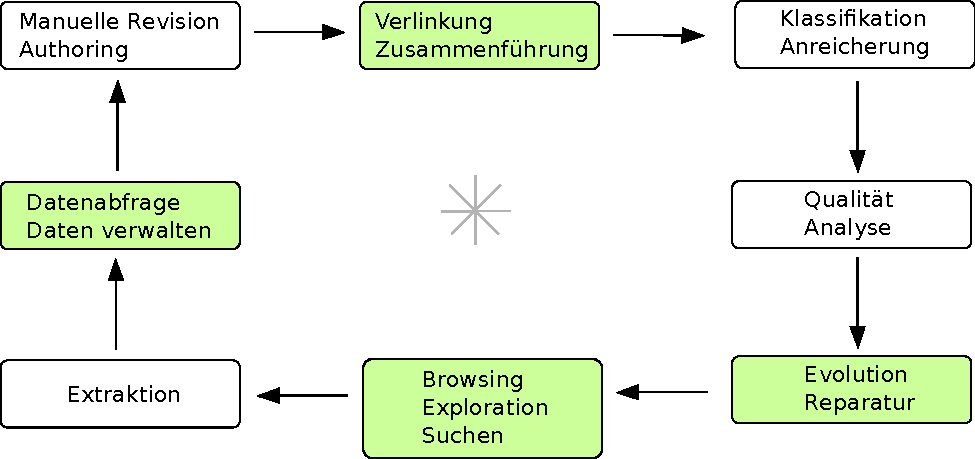
\includegraphics[width=12cm]{Statistics/LinkedDataLifeCycle.pdf}
    \caption{\small{Illustration des Linked Data Life-Cycle, basierend auf \cite[S. 3]{LINKEDDATA-LIFECYCLE}}.}
    \label{fig:Statistics_LinkedDataLifeCycle}
\end{figure}

\paragraph{Verlinkung / Zusammenführung}

Eine der schwierigsten Hauptaufgaben in Linked Data ist die (semi-)automatische Erstellung und Pflege von Links. Dafür werden zusätzlich Techniken, wie Machine Learning und Endbenutzer-Feedback genutzt. Bei der Zusammenführung geht es vordergründig um die Datenintegration, ähnlich wie im Bereich der Datenbanken. Hier spielen Schema-Integration und Konsistenzprüfung eine wichtige Rolle.

\paragraph{Evolution / Reparatur} 

Daten im Internet sind einer permanenter Veränderung unterworfen. Aus diesem Grund müssen Mechanismen zur Anwendung kommen, welche diese Veränderung unterstützen, aber die gleichzeitig stabilisieren. Diese Mechanismen sollten zudem Veränderungen an den RDF-Daten transparent und nachvollziehbar halten.

\paragraph{Browsen / Exploration / Suchen} 

In der Regel wird der Benutzer die RDF-Daten einer Linked Data Anwendung nicht zu Gesicht bekommen. Aus diesem Grund ist es wichtig, dass entsprechende Benutzerschnittstellen und Werkzeuge geschaffen werden, um eine adäquate Exploration und Suche in den Daten zu ermöglichen. Neben einer Benutzeroberfläche sollten Alternativen geschaffen werden, welche Exploration und Browsing auf Triple-Ebene ermöglichen.

\paragraph{Datenabfrage / Daten verwalten} 

Die Datenverwaltung von RDF-Daten findet in sogenannten Triple- oder Quad-Stores statt. Diese Art von Datenbanken legen ihre Daten in Form von Tripeln oder Quadrupeln ab. Dabei nutzen sie eine andere Abfragesprache als Relationale Datenbanksysteme, nämlich die Sprache SPARQL (\textit{SPARQL Protocol and RDF Query Language})\cite{SPARQL-SPEC}, in welcher man Abfragen in Form von Mustern formuliert.

%
% SS
%
\newpage
\subsection{Begriffserklärung und Herleitung des Mashup}
\label{sec:chapterBasicsMashup}

Wenn man sich heutzutage durch das Internet bewegt, stößt man zwangsläufig auf den Begriff des \emph{Mashup}. In diesem Kapitel soll es um die Erörterung der Frage gehen, was alles hinter dem Begriff Mashup steht. Eine breitgefächerte Erläuterung des Begriffes soll dem Verständnis helfen.

%
% Zitat
%
\begin{quote}
    \emph{The confusion even starts when looking for a generic definition of mashups. The definitions proposed in the literature span technical, business (in sense of economic) or industry perspectives.} \\ \cite[S. 1]{MASHUP-ELUCID}
\end{quote}

\noindent
Am Anfang wird der Begriff im Zusammenhang mit dem Internet vorgestellt. Danach folgt eine Übersicht über die Verwendung von Mashup's in der realen Welt. Abschließend werden Parallelen zwischen den beiden Welten gezogen und die dahinterstehenden Konzepte erläutert. Dieses Vorgehen wurde aus dem Grund gewählt, weil der Begriff Mashup einerseits sehr unterschiedlich definiert wird und andererseits die zugehörige Thematik recht komplex ist. Ziel ist es, dass der Leser die Konzepte und Techniken kennenlernt, die bei einem Mashup zur Anwendung kommen. Der Grund dafür ist, dass spätere Kapitel auf diesen Konzepten aufbauen.


%
% SSS
%
\subsubsection{Mashup im Internet}

Stefan Sonvilla-Weiss\footnote{\url{https://reseda.taik.fi/Taik/jsp/taik/Researcher.jsp?id=990834}}, Professor für Kommunikation- und Bildungstechnologien in Visuellen Medien, definiert den Begriff des \textit{Mashup im Internet} folgendermaßen:

%
% Kommentar
%
\com{Mashup \\ (Internet)}

%
% Zitat
%
\begin{quote}
    \emph{[...] the definition of mashup, which in Web developments denotes a combination of data or functionality from two or more external sources to create a new service (in the case of this compilation hopefully new insights), [...]} \\ \cite[S. 8]{MASHUP-REMIX-RECOM}
\end{quote}

\noindent 
Ohne das Zitat komplett zu übersetzen, bedeutet es, dass man verschiedene externe Quellen in einem neuen System zusammenführt mit dem Ziel, daraufhin neue Einsichten zu gewinnen. Es folgt eine andere Definition des Begriffs:

%
% Zitat
%
\begin{quote}
    \emph{Mashup's are typically simple web applications that, instead of being coded from scratch, are developed by integrating and reusing available data, functionalities, or pieces of user interfaces accessible over the Web.} \\
    \cite[S. 491]{MASHUP-DEVELOPTOOLS}
\end{quote}

\noindent
Laut diesem Zitat wird ein Mashup als Programm angesehen, welches aus fremden Daten und Funktionen besteht. 

\newpage
\noindent
Dabei liegt der Fokus auf der Wiederverwendung von anderen Quellen, wobei neben den Daten an sich, auch fremde Funktionen und sogar Teile von Benutzerschnittstellen weitergenutzt werden können. Bei beiden Definitionen wurden einige Begriffe nur unzureichend erläutert, weshalb dies nun nachgeholt wird.

Was bedeuten in diesem Zusammenhang \textit{externe Quellen}?\com{Externe\\ Quelle} Damit ist erst einmal jede digitale Quelle gemeint, welche Daten oder Funktionen, in Form von Algorithmen, über das Internet bereitstellt. In der Regel sind das Dienste (englisch \textit{Service}), welche über eine öffentlich zugängliche Schnittstelle Zugang zu ihren Daten und Algorithmen bieten. Der Begriff \textit{extern} rührt daher, dass man die abgefragten Daten und Informationen an einem Punkt zusammenführt und weiterverarbeitet. Dieser Punkt kann ein einfaches Programm sein oder ein Webservice, ein Dienst nutzbar über das Internet. Alle Dienste, die dabei nicht Teil des eigenen Programms oder Webservices sind, werden als extern bezeichnet.

In beiden Zitaten ist von Daten die Rede, die man abfragt, neu kombiniert und weiterverarbeitet. Mit Daten sind \textit{maschinenlesbare} Informationen gemeint. Dieser Punkt scheint auf den ersten Blick trivial, aber es gibt Datenquellen, welche Daten in einer Form bereitstellen, welche es nur mit vergleichsweise hohem Aufwand möglich machen, die enthaltenen Informationen zu extrahieren. Als Beispiel seien eingescannte Bilder mit handschriftlichen Notizen genannt, welche eine Texterkennungssoftware nötig machen.

%
% SS
%
\subsubsection{Mashup's in der materiellen Welt}

In der materiellen Welt findet man ebenfalls die Prinzipien eines Mashup vor. Dieses Unterkapitel soll  einen Überblick über die Verwendung des Begriffs in der materiellen Welt vorstellen. Auch wenn sich das Thema der Arbeit um die Nutzung von Mashup's im Internet dreht, so ist es dem Verständnis der Thematik sehr dienlich, einen kurzen Exkurs zur Verwendung von Mashup's in der materiellen Welt durchzuführen.

\begin{quote}
    \emph{The term mashup has its roots in the musical domain referring to artists that mix several pieces of music, usually from different musical styles, into one single record. [...] this term has been generalized and brought to other domains introducing the idea of derivating a new work by mixing two or more pieces.} \\
    \cite[S. 1 und 2]{MASHUP-ELUCID}
\end{quote}

\noindent
Laut dem obigen Zitat kommt der Begriff des Mashup\com{Ursprung Mashup} aus dem Bereich der Komposition von Liedern. In diesem Zusammenhang ist die Verwendung von verschiedenen Stilrichtungen gemeint, die in einem neuen Stück zusammengeführt werden. Ergänzend dazu folgendes Zitat:

%
% Zitat
%
\begin{quote}
    \emph{[...] these practices certain kinds of techniques (collage, montage, sampling, etc.) and different forms of appropriations within specific socio-cultural contexts [...]} \\ 
    \cite[S. 8]{MASHUP-REMIX-RECOM}
\end{quote}

\noindent
Neben der Musik findet man die Prinzipien, die beim Anfertigen eines Mashup's verwendet werden, auch in anderen Gebieten wieder. Als Prinzipien können dabei das Anfertigen von Collagen und Montagen gelten, aber auch das Ausprobieren. Mehr über die Begriffe der Montage und Collage aus dem Bereich der Kunst unter \cite[S. 11, S. 36]{COLLAGE-MONTAGE}.

Bei der Verwendung dieser Prinzipien muss man unterscheiden zwischen dem\com{Prinzip:\\ Eigenständiges Werk} Anfertigen eigenständiger Werke und der Erweiterung bzw. Modifikation eines bestehenden. Bei einem eigenständigen Werk gibt es ein Alleinstellungsmerkmal, welches es von anderen Werken abgrenzbar macht. Bei letzterem gibt es dieses Alleinstellungsmerkmal nicht.

Basierend auf dem folgenden Zitat kann man aus Werken, welche auf\com{Prinzip: \\Original erkennbar} anderen aufbauen, in der Regel auch das Original wieder extrahieren, also wiedererkennen. Es kann hier unterstellt werden, dass es bei der Modifikation eines bestehenden Werkes nicht gewollt ist, dass das Original unkenntlich wird.

\begin{quote}
    \emph{Mashup's [...] put together different information, media, or objects without changing their original source of information, i.e. the original format remains the same and can be retraced as the original form and content, although recombined in different new designs and contexts.} \cite[S. 9]{MASHUP-REMIX-RECOM}
\end{quote}

\noindent
Es kann aber durchaus gewollt sein, dass das, was von der Originalquelle genutzt wird, sei es die Quelle selbst oder deren Format, erhalten bleibt. Zusammenfassend lässt sich Folgendes festhalten: Der Ursprung des Mashup-Begriffs liegt in der Musik, doch er wird auch sehr stark in verschiedenen Formen in der Kultur und Kunst verwendet. Dabei kommen eine Reihe von Prinzipien bei der Anfertigung von Mashup's zum Einsatz. Dazu zählen die Collage und Montage sowie das Ausprobieren. Man kann bei Mashup's unterscheiden zwischen eigenständigen Werken und Werken, bei denen das darunterliegende Original noch (mehr oder weniger stark) erkennbar ist.

%
% SS
%
\subsubsection{Parallelen zwischen der digitalen und analogen Welt}

Bisher wurde über Mashup's in der digitalen und materiellen Welt referiert. Dabei wurden Prinzipien und Techniken vorgestellt, die in der Praxis unterschiedlich ausgeprägt sind. Um den Schulterschluss zu schaffen, werden nun die Parallelen zwischen den beiden Welten aufgezeigt.

Beginnen wir damit, dass man bei einem Mashup oft das Original erkennen kann, falls es aus einem anderen Werk hervorgegangen ist. Dies kann man sowohl bei Kunstgegenständen, als auch bei Print- und Audiovisuellen Medien vorfinden. Damit einher geht der Aspekt, dass die verwendeten Inhalte zur Erstellung eines Mashup gewissermaßen die Reputation der Quelle erben und sie auf das neue Werk übertragen.

Weiterhin stand die Kombination aus verschiedenen Medien, Print- oder Audiovisuellen Medien im Vordergrund. 


\newpage 
\noindent
In der digitalen Welt soll aufgrund der Vermischung verschiedener Quellen eine Kompilation entstehen, welche dem Betrachter einen Erkenntnisgewinn oder unmittelbaren Nutzen beschert. Dieser Anspruch war in der materiellen Welt nicht vordergründig. Dabei lag der Schwerpunkt auf der Betrachtung eines Themas aus einer anderen Sichtweise, sei es im auditiven, literarischen oder visuellen Sinne. Man kombiniert somit nicht wahllos Quellen, sondern wählt diese unter bestimmten Gesichtspunkten, aus um dem Betrachter etwas Bestimmtes damit zu sagen.

Es wurden Aspekte unserer Gesellschaft aufgezeigt, in denen die Thematik des Mashup allgegenwärtig ist. Man findet sie überall, sei es beim Radio hören oder Surfen im Internet. Um diesen Teil des Kapitels abzuschließen, sei ein Zitat von Bertold Brecht erwähnt:

\begin{quote}
    \emph{Der Rundfunk ist aus einem Distributionsapparat in einen Kommunikationsapparat zu verwandeln. [...] er wäre es, wenn er es verstünde, nicht nur auszusenden, sondern auch zu empfangen, also den Zuhörer nicht nur hören, sondern auch sprechen zu machen und ihn nicht zu isolieren, sondern ihn in
Beziehung zu setzen.} \\ 
\cite[S. 260]{BRECHT-RADIO}
\end{quote}

\noindent 
Dabei geht es um das Medium Radio und dass es laut Bertold Brecht die Möglichkeit bietet, die künstliche Grenze zwischen Konsument und Produzent aufzuheben. Jeder kann theoretisch selbst eine Radiostation gründen und seine Inhalte ausstrahlen. Die Plattform Youtube\footnote{\url{http://www.youtube.com}} treibt diese Idee in der digitalen Welt auf die Spitze, in dem sie nicht nur Klang- und Sprachinhalte bereitstellt, sondern auch visuelle Inhalte gesendet und empfangen werden können. Dabei erstellt der Produzent ein Mashup und der Konsument ist derjenige, der das Mashup abfragt und dessen Inhalte nutzt. Dabei gehen beide wechselseitige Beziehungen ein und können ihre Arbeit gegenseitig befruchten.


%
% SS
%
\subsubsection{Vertiefende Betrachtung von Mashup's im Internet}

Nach einer breitgefächerten Sicht auf das Thema des Mashup in der analogen und digitalen Welt, folgt nun eine vertiefende Betrachtung eines Mashup im Internet. Dazu folgendes Zitat:

%
% Zitat
%
\begin{quote} 
    \emph{[...] a mashup as a Web-based application that is created by combining and processing on-line third party resources, that contribute with data, presentation or functionality.} \\
    \cite[S. 2]{MASHUP-DEVELOPTOOLS}
\end{quote}

\noindent
Laut dem Zitat ist ein Mashup eine sich im Internet befindliche Software, welche durch die Verarbeitung von fremden Datenquellen eigene Präsentationen der Daten bereitstellt. Die Autoren weisen im Text nach diesem Zitat noch darauf hin, dass hier mit den sogenannten \emph{third party resources} jede im Internet verfügbare Quelle gemeint ist, im Sinne einer API oder einem Webservice. Weiterhin ist ein Mashup eine Anwendung, welche auf der \textit{Serviceorientierten Architektur} (SOA)\com{SOA}\cite{SOA-INTRO} basiert. 


\newpage 
\noindent
Zum besseren Verständnis wird im Folgenden eine kurze Einführung in SOA erfolgen, um darauf aufbauend die besonderen Charakteristika eines Mashup herauszuarbeiten. Die Serviceorientierte Architektur bezeichnet die Form einer Architektur aus der Informationstechnik und beschreibt dabei, wie Programme oder Services, hier auch als Software-Agenten bezeichnet, miteinander interagieren sollen. Ziel ist, dass es zwischen diesen Software-Agenten nur eine lose Kopplung gibt. Als lose gekoppelt bezeichnet man eine Verbindung zwischen zwei oder mehreren Software-Agenten, wenn eine Änderung innerhalb eines Agenten nur lokale Auswirkungen hat. Das heißt, dass die angekoppelten Agenten aufgrund der Änderung nicht angepasst werden müssen. Abhängigkeiten werden zudem nur zu dem Grad eingegangen, wie es für die Kommunikation untereinander nötig ist. \cite[S. 1 ff]{SOA-WHAT-IS} \cite[S. 131]{LOOSELY-COUPLED} Ein weiteres Merkmal von SOA-basierten Anwendungen ist, dass jeder teilnehmende Software-Agent die Hoheit über die von ihm bereitgestellten Dienste besitzt. Es ist aber auch möglich, dass ein Agent weitere Agenten steuert und so indirekt die Hoheit über deren Dienste besitzt.

Ein Mashup ist eine spezielle Form einer SOA-basierten Anwendung, denn man erstellt in der Regel nur das Mashup und definiert die Schnittstellen, über die die Außenwelt mit ihm kommunizieren kann. Es muss zur Erstellung des Mashup noch keine Nutzer geben. Der Einsatzzweck einer SOA-basierten Anwendung ist nicht vorgeschrieben, ein Mashup hingegen ist für den Einsatz im Internet konzipiert. Weiterhin können die fremden Quellen bei Mashup's neben Diensten, auch andere Formen annehmen, wie z.B. reine Datenquellen. \cite[S. 2]{MASHUP-ELUCID}

Im Folgenden werden die wichtigsten SOA-Prinzipien aufgezählt und deren Ausprägung bei Mashup's vorgestellt. Diese Vorarbeit dient später dazu, die Software \mbox{CubeViz} dahingehend zu überprüfen, ob sie die Kriterien eines Mashup's erfüllt.


%
% P
%
\paragraph{Lose Kopplung und maximale Abkapselung} 

Die lose Kopplung\com{Auflistung \\ der SOA- \\Prinzipien} zwischen interagierenden Software-Agenten ist eines der Hauptmerkmale von SOA-Anwendungen. Aus dieser Anforderung folgt, dass sich die Agenten nur über einen minimalen Satz an Nachrichten mit begrenzter Semantik austauschen können. Bei Mashup's herrscht keinerlei Kopplung und die Dienste sind völlig unabhängig voneinander. Kombiniert man jedoch mehrere Mashup's zu einem neuen, dann kommt es wieder zu einer Kopplung zwischen den Mashup's, welche aber nur für den Datenaustausch zwischen den Mashup's nötig ist. 

Einher mit der losen Kopplung zwischen den SOA-Agenten geht die maximale Abkapselung eines SOA-Agenten von seiner Außenwelt. Die bereits erwähnten öffentlich zugänglichen Schnittstellen bilden die einzige Möglichkeit, mit den Diensten des Agenten kommunizieren zu können, denn die internen Abläufen und die  Programmlogik sind nach außen hin verborgen. Dieses Prinzip ist bei Mashup's voll ausgeprägt. \cite[S. 2]{MASHUP-ELUCID} \cite[S. 2]{SOA-WHAT-IS}

\paragraph{Gute Auffindbarkeit und erleichterte Wiederverwendung} 

Es gibt Auszeichnungssprachen, welche zur Beschreibung von SOA-basierten Diensten verwendet werden. Das Ziel dabei ist, dass ausreichend Informationen über den Dienst selbst und seine Verwendungszwecke vorliegen, sodass er einfach gefunden und wiederverwendet werden kann. 

\newpage 
\noindent
Bei Mashup's wird gefordert, dass die Informationen \textit{maschinenlesbar} sind und einfach weiterverarbeitet werden können.

Eine gute Beschreibung und Auffindbarkeit unterstützen die Wiederverwendung von Diensten ungemein. Jeder einzelne Dienst hat die Aufgabe ein spezifisches Problem oder Aufgabenfeld zu lösen. Dazu stellt er Eingangsparameter bereit und liefert im Erfolgsfall eine Ergebnismenge zurück. Wenn die Vorbedingungen und der mögliche Nutzen von Diensten ausreichend dokumentiert sind, dann unterstützt das dessen Wiederverwendung. Im Internet befindliche Mashup's haben die Möglichkeit, die Wiederverwendung zu unterstützen, indem sie gut auffindbar sind und eine gute Dokumentation ihrer Schnittstellen bereitstellen. \cite[S. 2]{MASHUP-ELUCID}

%
% P
%
\paragraph{Dienst-Autonomie} 

Wie bereits erwähnt, unterstützt die lose Kopplung die Autonomie der Software-Agenten. Mit Autonomie ist hier die Hoheit eines Agenten über die von ihm bereitgestellten Dienste gemeint. Dies wird bei den Mashup's ebenfalls übernommen, wobei ein Mashup nur die Hoheit über den eigenen Dienst und dessen bereitgestellte Daten besitzt. 


%
% P
%
\paragraph{Art der Nutzung}

Die Autoren des Papers \cite{MASHUP-ELUCID} führen ein weiteres Prinzip speziell für Mashup's ein. Dabei geht es darum, wie und auf welche Art ein Dienst genutzt wird. Die Einführung wird damit begründet, dass Mashup's im Internet eine größere Reichweite besitzen und viele Benutzer ansprechen können.

Neben den Softwareentwicklern, soll es auch Personen ohne Programmiererfahrung möglich sein, Mashup's zu benutzen. Dabei spielen sie nicht unbedingt eine Rolle in der aktiven Nutzung der Dienste, aber oft bei der Weiterentwicklung dieser, z.B. durch Feedback oder das Melden von Fehlern. Um ein Mashup einer breiten Öffentlichkeit zugänglich zu machen, müssen die -- oft eher technischen -- Einstiegsbarrieren niedrig sein und der Funktionsumfang sollte durch eine ausreichende Dokumentation erläutert werden.

%
% SS
%
\subsubsection{Kategorien eines Mashup}

Nachdem das Mashup von einer SOA-Anwendung abgegrenzt wurde, soll es nun um die Klassifikation eines Mashup gehen. Dazu werden drei Kategorien vorgestellt und diese Aufstellung soll später für die Kategorisierung von CubeViz benutzt werden.

%
% P
%
\paragraph{Consumer Mashup}

Ein \emph{Consumer Mashup}\com{Konsumenten-Mashup} heißt übersetzt soviel wie \textit{Konsumenten-Mashup} und ist gedacht für die allgemeine Öffentlichkeit. Charakteristisch bei dieser Art ist, dass man sie ohne weiteres über den Browser benutzen kann und sie an die eigenen Bedürfnisse anpassbar ist. Mit dem letzten Punkt ist gemeint, dass man die Auswahl der anzuzeigenden Daten einschränken kann. \cite[S. 2]{MASHUP-AND-ENTERP}

Als Beispiel für ein solches Mashup sei Google Maps genannt, auch wenn es kein reines Consumer Mashup ist. Es bietet eine leicht zu bedienende Oberfläche für den Webbrowser, mit der man auf geographische Daten zugreifen kann. 


\newpage 
\noindent
Weiterhin bietet es die Möglichkeit, auf einer Landkarte alle Firmen einer Stadt zu sehen oder eine Route zwischen zwei Städten zu berechnen und darzustellen. \cite[S. 3]{GOOGLE-MAPS}


%
% P
%
\paragraph{Data Mashup}

Ein \emph{Data Mashup},\com{Daten-\\Mashup} übersetzt \textit{Daten-Mashup}, führt Daten aus verschiedenen Quellen an einem Punkt zusammen und gewährt über eine Schnittstelle Zugriff auf die Daten. Hierbei liegt der Fokus auf der Schaffung einer aggregierten Visualisierung aller genutzten Quellen. \cite[S. 2]{MASHUP-AND-ENTERP} 

%
% P
%
\paragraph{Business Mashup's}

\emph{Business Mashup's}, übersetzt \textit{Geschäfts-Mashup's}\com{Geschäfts-\\Mashup}, stellen die Daten in einer bestimmten Art von Visualisierung dar. Weiterhin werden sie bevorzugt bei agilen Projekten genutzt, wo eine Kollaboration zwischen Entwicklern und Unternehmen nötig ist, um Anforderungen zu definieren und implementieren. 

Diese Art von Mashup's unterscheidet sich von Konsumenten-Mashup's durch eine andere Ebene der Integration von Softwareumgebungen der beteiligten Unternehmen und aufgrund der Nutzung von Sicherheits- und Zugangskontrollsoftware, damit Benutzer kollaborieren können. Ein anderes Unterscheidungsmerkmal ist der seit einigen Jahren auftretende Trend, kommerzielle Software als einen kostenpflichtigen Service anzubieten, sogenanntes \textit{Software as a Service} (SaaS)\cite{SAAS-INTRO}.\com{SaaS} Dabei stellt ein Unternehmen die Software in Form einer Webseite bereit, die über einen Browser genutzt werden kann. Man trennt dabei quasi den \textit{Besitz} der Software von seiner \textit{Nutzung}.

Die Software selbst läuft dabei auf den Servern des Unternehmens. Ein Grund für die verstärkte Nutzung solcher Angebote ist es, dass man als Nutzer damit im Vergleich zu herkömmlicher Software Geld sparen kann, weil beispielsweise lokale Installationen entfallen und damit auch kostenintensive Hardware nicht angeschafft und gewartet werden muss. \cite[S. 2]{MASHUP-AND-ENTERP}


%
% SSS
%
\subsubsection{Ebenen eines Mashup}

Neben einer Kategorisierung von Mashup's, ist auch eine Einteilung in verschiedene Ebenen möglich. Im Folgenden werden drei Ebenen vorgestellt, die den drei Komponenten des Model-Controller-View-Musters (MVC)\cite{MVC-ORIGIN} entsprechen: Die Daten-, Prozess- und Präsentationsebene. Die Informationen über die einzelnen Ebenen basieren auf \cite{MASHUP-DATA-INTERGRATION}. Diese Ausführungen werden später bei der Beschreibung der Software CubeViz und dessen Bestandteile nochmal wichtig.

%
% P
%
\paragraph{Datenebene}

Auf dieser Ebene finden alle Operationen zur Datenmanipulation statt, wie beispielsweise die Filterung und Konvertierung, um Daten aus verschiedenen Quellen integrieren zu können. Dabei werden Daten aus verschiedenen Quellen zusammengeführt, wobei die Quellen in der Regel ein \textit{REST}- oder \textit{SOAP}-Service, oder über das HTTP bzw. \textit{XML RPC} abfragbar sind. 


\newpage 
\noindent
Da die Daten aus verschiedenen Quellen stammen, können sie sowohl in strukturierter als auch unstrukturierter Form vorliegen. Daher liegt die Herausforderung darin, diese Daten in ein einheitliches Schema zusammenzuführen. Strukturierte Daten, wie XML, besitzen ein definiertes Datenmodell, wogegen unstrukturierte Daten keines besitzen und daher vorher verarbeitet werden müssen, um ihre \textit{Semantik} zu erfassen. Danach kann man aus ihnen strukturierte Daten herstellen.


%
% P
%
\paragraph{Prozessebene}

Auf der Prozessebene werden die beteiligten Anwendungen integriert. Nutzt man dafür Programmiersprachen, so erfolgt die Integration der verschiedenen Anwendungen in der Regel durch den Aufruf der jeweiligen API's. Eine andere Möglichkeit bestünde darin, sie über sogenannte Workflow-Sprachen zu integrieren, was aber im Folgenden nicht von Belang ist.

%
% P
%
\paragraph{Präsentationsebene}

Auf der letzten Ebene wird eine Schnittstelle zur Benutzer-\mbox{interaktion} bereitgestellt. Dazu zählt die Abfrage von Benutzereingaben und das Anzeigen der Abfrage-Ergebnisse. Im Internet werden dafür in der Regel \textit{HTML}, \textit{JavaScript} und \textit{CSS} genutzt. Es gibt verschiedene Darstellungsformen: Sie reichen von einfachen Listen über interaktive Programme bis hin zu domänenspezifischen Darstellungen, wie einer Landkarte für geographische Informationen.

Je nachdem, ob die Anwendung serverseitig- oder clientseitig ausgelegt ist, kommt eine andere Art der Präsentation zum Tragen. \textit{Serverseitige} Mashup's\com{Serverseitig} bekommen eine Benutzereingabe, z.B. über ein ausgefülltes Formular, verarbeiten diese und senden ein Ergebnis an den Benutzer zurück. Dabei werden die Datenquellen und Dienste auf dem Server integriert. Der Server nimmt dabei die Rolle eines Proxy ein und bildet so die Schnittstelle zwischen den Datenquellen und der Mashup-Anwendung. 

Die andere Art sind \textit{clientseitige} Mashup's.\com{Clientseitig} Hierbei findet die Datenintegration auf dem Client statt, welcher in der Regel ein Browser ist. Über JavaScript und die Technik \textit{Asynchronous JavaScript and XML} (AJAX)\cite{AJAX} werden die nötigen Anfragen an den Server geschickt und die ermittelten Ergebnisse im Client verarbeitet, integriert und angezeigt. Mit fortschreitender Entwicklung werden die API's der Browser immer mächtiger und erlauben immer umfangreichere Funktionen. Damit wird die Notwendigkeit geringer, den Server für konkrete Aufgaben zu benutzen. 

Man kann die beiden Mashup-Arten nicht vollständig voneinander trennen, denn in beiden sind jeweils Server und Client involviert. Es kommt auf den Entwickler an, zu welchem Grad der Server und der Client jeweils involviert sein sollen.


%
% SS
%
\subsection{Linked Data + Mashup = Linked Data Mashup}
\label{sec:chapterBasicsLinkedDataMashup}

Nach einer umfangreichen Vorstellung der Mashup's, werden nun die Begriffe \emph{Linked Data} und \emph{Mashup} im Begriff \emph{Linked Data Mashup} zusammengeführt. 


\newpage 
\noindent
Dieser wird folgendermaßen definiert: 

\begin{quote}
    \textit{Ein Linked Data Mashup ist ein im Internet zugänglicher Dienst für eine bestimmte Domäne. Diese Domäne ist durch eine Ontologie definiert sowie einer Menge von Linked Data Quellen, welche über Anwendungsontologien modelliert wurden.}\\(Basiert auf Übersetzung von \cite[S. 1]{MASHUP-LINKEDDATA})
\end{quote}

\noindent
Die obige Definition wird noch eingeschränkt dadurch, dass die Anwendungsontologien eine Teilmenge der Domänenontologie sind und dass das Linked Data Mashup Zugriff auf die Vokabulare der Anwendungsontologien, aber nicht auf deren Regeln, besitzt.

Man kann nicht davon ausgehen, dass die empfangenen Daten der Linked Data Quellen konsistent mit den Regeln der Domänen-Ontologie sind. Es gibt noch nicht einmal eine Garantie, dass man von Linked Data Quellen überhaupt konsistente Daten empfängt. Und selbst wenn alle Linked Data Quellen konsistente Daten liefern, so kann es sein, dass diese Daten zusammen inkonsistent werden. Aus diesem Grund wird gefordert, dass ein Linked Data Mashup die empfangenen Daten analysiert, um inkonsistente Daten zu finden und zu isolieren. Ein Linked Data Mashup ist also nicht bloß eine einfache Datenquelle, welche RDF-Daten bereitstellt. (Näheres dazu in \cite{MASHUP-LINKEDDATA})

Für diese Arbeit wurden die genannten Einschränkungen und Anforderungen an Linked Data Mashups abgeschwächt. Es werden nur Quellen betrachtet, die statistische Daten bereitstellen, wobei die Daten auf dem DataCube-Vokabular basieren, welches später noch erläutert wird. Die Anforderungen an die Inkonsistenz der Daten wird abgeschwächt. Es wird lediglich gefordert, dass die DataCube-Elemente und ihre Beziehungen untereinander valide sind. Der Grund für die Abschwächung liegt darin, weil CubeViz nur mit Daten im DataCube-Format umgehen kann. Der Vollständigkeit halber soll hier noch angemerkt sein, dass CubeViz für die Konsistenz-Überprüfung eine eigene Benutzeroberfläche bereitstellt. Bei der Entwicklung von CubeViz wurde der Wert jedoch weniger auf die Qualitätsanalyse der genutzten Daten als auf deren Visualisierung gelegt.

Die eingangs erwähnten Prinzipien und Techniken bei der Mashup-Erstellung sind bei einem Linked Data Mashup ebenfalls anwendbar. Im Folgenden werden die Prinzipien Montage/Collage, Eigenständigkeit von Werken und die Erkennung von Originalen auf Linked Data Mashup's übertragen.

%
% SSS
%
\subsubsection{Prinzip der Montage}
\label{sec:MashupPrinciple-Adaption}

Beginnen wir mit der Montage und Collage. Bei einem Linked Data Mashup werden aus verschiedenen Linked Data Quellen RDF-Daten zusammengeführt. Bei der Zusammenführung verschiedener Datenquellen kann es zur Filterung, Integration und Veränderung der empfangenen Daten kommen. Was auch immer passiert, allein schon durch die Zusammenführung der Tripel erhält der auf diese Weise erstellte Graph eine neue Semantik. 


%
% SSS
%
\subsubsection{Prinzip der Eigenständigkeit von Werken}
\label{sec:MashupPrinciple-Sovereignty}

Eingangs wurde definiert, dass ein eigenständiges Werk ein Alleinstellungsmerkmal besitzt und deswegen von anderen Werken abgegrenzt werden kann. Werke, die nicht eigenständig sind, besitzen ein solches Merkmal nicht und benötigen daher eine Referenz auf das Werk, auf dem sie basieren. Wie diese Referenz aussieht, unterscheidet sich je nach Werk und Art der Kunstrichtung. Hier soll nur angenommen werden, dass diese in irgendeiner Form existiert und der Betrachter eine Verbindung zwischen Original und montiertem Werk herstellen kann. Dieses Prinzip lässt sich nur bedingt auf Linked Data Mashup's übertragen. Der Grund dafür ist, dass ein solcher Dienst die Eigenschaft der maximalen Abkapselung besitzt, also dem Verbergen von internen Abläufen und der Programmlogik von der Außenwelt. Daher ist es für den Betrachter in der Regel nicht möglich zu erfahren, welche Linked Data Quellen der Dienst benutzt und welche Quellen diese wiederum nutzen. Nichtsdestotrotz kann man basierend auf den empfangenen Daten des Linked Data Mashup's sowie der genutzten Domänenontologie Rückschlüsse auf die Ursprünge gewisser Daten ziehen. Aufgrund der RDF-Datenstruktur erhält der während einer Zusammenführung im Mashup erstellte Graph eine neue Semantik. Aus der mangelnden Abgrenzbarkeit der RDF-Daten und der maximalen Abkapselung von Linked Data Mashup's wird geschlussfolgert, dass es eigenständige Werke, wie beispielsweise in der bildenden Kunst, nicht geben kann.


%
% SSS
%
\subsubsection{Prinzip der Erkennbarkeit von Originalen}
\label{sec:MashupPrinciple-Original}
\label{req:F10source}

Das \nameref{sec:MashupPrinciple-Original} ist eng verbunden mit dem \nameref{sec:MashupPrinciple-Sovereignty}. Ein nicht-eigenständiges Werk besitzt immer eine Referenz auf das Original, auf dem es beruht. Überträgt man dies auf Linked Data Mashup's, so bedeutet das, dass man als Benutzer eines solchen Dienstes in die Lage versetzt wird, die Quellen der einzelnen RDF-Tripel zu \emph{erkennen} (\textit{F-10})\com{Anforderung \\ F-10, S. \pageref{req:F10}}. Wobei man hier unterscheiden muss zwischen den abgefragten Linked Data Quellen, den genutzten Namensräumen in den URI's der Tripel sowie einer Datenbank innerhalb des Linked Data Mashup's. Ersteres und letzteres kann der Benutzer wohl im besten Falle nur schätzen, aber die genutzten Namensräume sind bei Betrachtung der reinen RDF-Daten immer gegeben. Besitzt der Benutzer zusätzliches Expertenwissen über das Linked Data Mashup selbst und kennt er dessen genutzte Linked Data Quellen, so kann ihn das in die Lage versetzen, die \emph{Originaldaten} zu rekonstruieren.

Im Zusammenhang mit fremden Datenquellen wird man oft vor eine Reihe von Fragen gestellt \cite[S. 19]{LINKEDDATA-ABOUT}:

\begin{itemize}
	\item Kann man den Daten vertrauen?\com{Trust} Sind die Quellen glaubwürdig? \\(Daten vertrauen, \textit{Trust})
	\item Woher\com{Provenance} kommen die Daten? Wie sind sie entstanden? Wer ist der Autor? \\(Herkunft der Daten, \textit{Provenance})
\end{itemize} 

\noindent
Diese Fragen bekommen spielen bei dem \nameref{sec:MashupPrinciple-Original} eine große Rolle. 


\newpage 
\noindent
Daneben beschreiben sie auch ein großes Problemfeld bei Linked Data, da es dort um die vordergründige Nutzung verteilter Datenquellen geht. Baut man auf fremden Daten auf, so muss man sicher sein, dass die Daten korrekt sind und später das halten, was sie versprechen. Aus diesem Grund muss es für den Nutzer immer ersichtlich sein, welche Daten woher kommen und ggf. wie sie zustande gekommen sind.\\

\noindent
Bis zu diesem Punkt sollte der Leser ausreichend Hintergrundwissen über die technischen Grundlagen dieser Arbeit erhalten haben. Es sollte klar geworden sein, welche Technologien für den Datenaustausch genutzt werden (Linked Data, Mashup) und in welcher Form die Daten (RDF) vorliegen können. Das Wissen über die Einteilung und den Aufbau von Mashup's ist ebenso hilfreich, wie die verwendeten Prinzipien und Techniken für deren Erstellung. Der Exkurs in andere Bereiche außerhalb der IT sollte einen Eindruck vermittelt haben, worin der Ursprung des Mashup-Gedanken liegt und wo er überall um uns herum Anwendung findet.

%
% SS
%
\subsection{Über die Applikation OntoWiki im Kontext dieser Arbeit}
\label{sec:chapterBasicsOW}

Die Web-Anwendung \textit{OntoWiki} kann dazu verwendet werden, um kollaborativ und verteilt Ontologien zu erstellen und weiterzuentwickeln. Es wurde von Dr. Sören \mbox{Auer} initiiert und seitdem aktiv von der Gemeinschaft weiterentwickelt. OntoWiki ist sowohl ein semantisches Daten-Wiki als auch ein Framework zur Publikation von Linked Data. Weiterhin bietet es sich als Basis für die Entwicklung eigener semantischer Applikationen an. Die semantischen Daten werden durch das Framework \textit{Erfurt}\footnote{\url{http://aksw.org/Projects/Erfurt.html}} verwaltet, welches eine Semantic Web API für soziale semantische Software darstellt und die Aufgabe hat, eine Brücke zwischen einer Applikation, in dem Falle OntoWiki, und einer Datenbank herzustellen. Dabei kann es mit verschiedenen Arten von Datenbanken umgehen, also sowohl mit relationalen Datenbanksystemen wie \textit{MySQL}\footnote{\url{https://www.mysql.com}}, als auch mit einem TripleStore wie \textit{Virtuoso}\footnote{\url{http://virtuoso.openlinksw.com}}. OntoWiki besitzt zwar einen monolithischen Kern, dieser stellt aber ein Komponentensystem bereit. Dadurch kann man eigene Komponenten aufsetzen und auf diese Weise den Kern erweitern. Weiterhin stellen Erfurt und das darauf aufbauende OntoWiki Funktionen für Komponenten bereit, damit sie semantische Daten aus der Datenbank abfragen und verarbeiten können. \cite{ONTOW}

Diese Arbeit legt ihren Fokus auf die Anpassung und Erweiterung der OntoWiki-Komponente CubeViz, einem RDF-Browser zur facettierten Exploration von semantischen statistischen Daten, welche im DataCube-Format vorliegen.\com{Kapitel \ref{sec:chapterCubeViz} \\ S. \pageref{sec:chapterCubeViz}} CubeViz selbst wird im Kapitel \ref{sec:chapterCubeViz} näher vorgestellt.

%
% SS
%
\subsection{Vorstellung des DataCube-Vokabulars}
\label{sec:chapterBasicsDC}

Im Folgenden wird auf das DataCube-Vokabular\cite{DATACUBE-SPEC} näher eingegangen, um den Leser mit den wichtigsten Grundbegriffen und Konzepten vertraut zu machen. Es ist eine Ontologie mit der man multidimensionale statistische Daten modellieren kann. Statistische Daten liegen hier in Form von Beobachtungspunkten vor. Ein Beobachtungspunkt ist dabei eine Messung mit einem konkreten Wert, welche zusätzliche Eigenschaften besitzt. Der Fokus dieses Vokabulars liegt dabei rein auf der Veröffentlichung von mehrdimensionalen statistischen Daten im Internet, unter Nutzung von RDF und Linked Data. Es folgt nun eine Reihe von kurzen, präzisen Erläuterungen der für diese Arbeit wichtigen Begriffe und Konzepte.


%
% SSS
%
\subsubsection{Datensatz: Eine Menge an statistischen Daten}

Der Begriff des \emph{Datensatzes} (im Vokabular \textit{DataSet}) ist von zentraler Bedeutung.\com{Datensatz \\[0.2cm] 
\includegraphics[width=0.32cm]{semicon/dataset3.pdf}} Ein Datensatz ist eine Art Container, der eine Menge an Beobachtungsdaten zu einer, wenn auch nur abstrakten, Beobachtung beinhaltet. Die Beobachtung kann dabei sowohl über einen konkreten Gegenstand sein, als auch etwas Abstraktes beschreiben.

Neben diesen Beobachtungsdaten werden diverse Metadaten erfasst, welche die Beobachtungsdaten klassifizieren und näher beschreiben. Zu einem Datensatz gehört immer eine \textit{Datenstruktur Definition} (im Vokabular \textit{Datastructure Definition}).\com{Datenstruktur Definition \\[0.2cm] 
\includegraphics[width=0.4cm]{semicon/dataStructureDefinition.pdf}} Sie stellt die Verbindung zwischen einem Datensatz mit seinen Beobachtungspunkten und den Metadaten bereit, welche die Beobachtungspunkte näher beschreiben. \\


%
% Code
%
\begin{verbatim}
   @prefix ex: <http://example.cubeviz.org/> .       
   @prefix rdfs: <http://www.w3.org/2000/01/rdf-schema#> .
   @prefix qb: <http://purl.org/linked-data/cube#> .
    
   # Datensatz
   ex:dataset a qb:DataSet ;
              rdfs:label "Datensatz" ;
              qb:structure ex:dsd .

   # Datenstruktur-Definition                   
   ex:dsd a cube:DataStructureDefinition ;
          rdfs:label "Datenstruktur-Definition" ;
          qb:component ex:geo, ex:time, ex:unit, ex:value .
\end{verbatim}

\noindent
Obiger Codeausschnitt definiert einen Datensatz mit einem Titel (\textit{rdfs:label}) und der zugehörigen Datenstruktur-Definition dsd. Die Datenstruktur-Definition besitzt neben einem Titel vier Verbindungen zu Komponenten: zwei Dimensionen (\textit{exCs:geo} und \textit{exCs:time}), Messwert (\textit{ex:value}) und Maßeinheit (\textit{exCs:unit}).



%
% SSS
%
\subsubsection{Dimension: Eindeutige Identifizierung eines Beobachtungspunktes}

Eine \textit{Dimension} \com{Dimension \\[0.2cm] 
\includegraphics[width=0.4cm]{semicon/dimension.pdf}} hat die Aufgabe, einen bestimmten Teil eines Beobachtungspunktes näher zu identifizieren. Sie besitzt eine endliche Menge an Dimensionselementen (im Vokabular \textit{Dimensionelement}), die dann später, statt der Dimension selber, an den Beobachtungspunkt angebunden werden. Jedem Beobachtungspunkt ist dabei genau ein Dimensionselement für jeweils eine Dimension zugeordnet. \\

% Abbildung
\begin{figure}[h!]
    \centering
    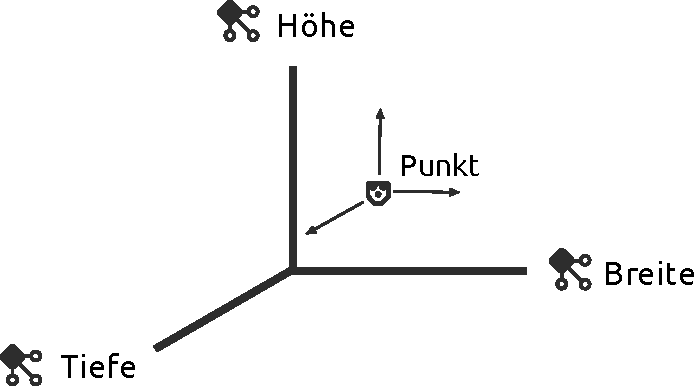
\includegraphics[width=7.5cm]{DataCube/DataCubeVocabulary_UnderstandingDimensionsIllustration.pdf}
    \caption{Ein Raum mit drei Dimensionen und einem Punkt darin.}
    \label{fig:DataCubeVocabulary_UnderstandingDimensionsIllustration}
\end{figure}

\noindent
Als Analogie dazu sei auf die Abbildung \ref{fig:DataCubeVocabulary_UnderstandingDimensionsIllustration} verwiesen, auf der ein dreidimensionales kartesisches Koordinatensystem zu sehen ist. Dieses besitzt die drei Achsen Breite, Höhe und Tiefe. Jede dieser Achsen kann als Dimension angesehen werden, wobei alle Punkte einer Achse bijektiv auf die Menge der natürlichen Zahlen abgebildet sein müssen. Soll heißen, jede Dimension enthält eine endliche Menge an Dimensionselementen und ist somit diskret und nicht stetig. Möchte man nun einen Punkt innerhalb dieses Koordinatensystems platzieren, so hat man die Werte für die Breite, Höhe und Tiefe zu setzen. Auf diese Weise ist jeder Punkt eindeutig identifizierbar. Ein ebensolcher Punkt entspricht dabei einem Beobachtungspunkt innerhalb eines Datensatzes.

%
% Code
%
\begin{verbatim}
    
   @prefix ex: <http://example.cubeviz.org/> .        
   @prefix rdfs: <http://www.w3.org/2000/01/rdf-schema#> .
   @prefix qb: <http://purl.org/linked-data/cube#> .
    
   # Dimension der Region
   ex:geo a qb:DimensionProperty ;
          rdfs:label "Region" .
        
   # Dimension der Zeit
   ex:date a qb:DimensionProperty ;
           rdfs:label "Zeit" .
\end{verbatim}

\noindent
Im obigen Codeausschnitt werden zwei Dimensionen definiert. Jede Dimension ist vom Typ \textit{DimensionProperty} und besitzt jeweils einen eigenen Titel.

%
% SSS
%
\subsubsection{Messwert: Gemessener Wert eines Beobachtungspunktes}

Im DataCube-Vokabular wird vorausgesetzt, dass alle Beobachtungspunkte innerhalb eines gültigen Datensatzes mindestens einen konkreten \textit{Messwert}\com{Messwert \\[0.2cm] 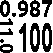
\includegraphics[width=0.5cm]{semicon/measure2.pdf}} (im Vokabular \mbox{\textit{Measure}}) besitzen. Jedem Beobachtungspunkt sind dabei ein Messwert und manchmal noch eine Maßeinheit zugeordnet. In der Regel ist ein Messwert eine Zahl, wobei Zeichenketten oder Sonstiges nicht ausgeschlossen sind.

%
% Code
%
\begin{verbatim}
    
    @prefix ex: <http://example.cubeviz.org/> .        
    @prefix rdfs: <http://www.w3.org/2000/01/rdf-schema#> .
    @prefix qb: <http://purl.org/linked-data/cube#> .
    
    # Messwert
    ex:value a qb:MeasureProperty ;
             rdfs:label "Population" .
\end{verbatim}

\noindent
Auf dem obigen Codeausschnitt ist ein Messwert beispielhaft definiert. Ein Messwert ist eine Ressource vom Typ \textit{MeasureProperty} und besitzt daneben oft noch einen Titel, im Beispiel mit \textit{Population} bezeichnet.

%
% SSS
%
\subsubsection{Maßeinheit: Zur Interpretation eines Messwertes}

Eine \textit{Maßeinheit}\com{Maßeinheit \\[0.2cm] 
\includegraphics[width=0.5cm]{semicon/attribute2.pdf}} (im Vokabular \textit{Attribute}) dient zur Interpretation eines vorliegenden Messwertes. Sie ist als einfache Zeichenkette betitelt und sollte kurz und prägnant beschreiben, was hinter dem Messwert steckt. So kann eine Maßeinheit auch für einen Faktor stehen, mit dem man den Messwert vor der Nutzung zu multiplizieren hat. Als Beispiel sei dazu der Messwert \textit{Bevölkerung eines Landes} und die Maßeinheit \textit{in Millionen} gegeben. Das würde dann bedeuten, dass jeder Wert über die Bevölkerungsangabe erst noch mit einer Million multipliziert werden muss, bevor er genutzt werden kann.\\


%
% Code
%
\begin{verbatim}    
   @prefix exProp: <http://example.cubeviz.org/properties/> .        
   @prefix rdfs: <http://www.w3.org/2000/01/rdf-schema#> .
   @prefix qb: <http://purl.org/linked-data/cube#> .
    
   # Maßeinheit
   exProp:unit a qb:AttributeProperty ;
               rdfs:label "in Millionen" .
\end{verbatim}

\noindent
In diesem Codeausschnitt wird eine Maßeinheit definiert. Diese ist vom Typ \textit{AttributeProperty} und trägt den Titel \textit{in Millionen}.

%
% SSS
%
\subsubsection{Beobachtungspunkt: Momentaufnahme während einer Beobachtung}

Bisher ist öfters der Begriff des \textit{Beobachtungspunktes}\com{Beobachtungs-punkt \\[0.2cm] 
\includegraphics[width=0.4cm]{semicon/observation.pdf}} (im Vokabular \textit{Observation}) gefallen. Dabei handelt es sich um eine Momentaufnahme während einer Beobachtung, bei der etwas gemessen wird. Sie setzt sich dabei aus einer endlichen Menge an Beobachtungspunkten zusammen, wobei an jedem Beobachtungspunkt die in zugehörigen Datenstruktur-Definition definierten Komponenten angehängt sein müssen.

Eingangs wurde erwähnt, dass der Fokus des DataCube-Vokabulars auf der Modellierung und Veröffentlichung von statistischen Daten, unter Nutzung von RDF und Linked Data, liegt. Ein Konzept von RDF ist die eindeutige Bezeichnung von Ressourcen über URI's, was dann ebenfalls für die Beobachtungspunkte gilt. Damit besitzt man die Möglichkeit, die einzelnen Beobachtungspunkte global eindeutig zu referenzieren und domänenübergreifend wiederzuverwenden. Spinnt man diesen Gedanken weiter, käme man zu einer Situation, in der Statistiker gemessene Werte global referenzieren und in Beziehung zueinander setzen können.

%
% Code
%
\begin{verbatim}
        
   @prefix ex: <http://example.cubeviz.org/> .        
   @prefix rdfs: <http://www.w3.org/2000/01/rdf-schema#> .
   @prefix qb: <http://purl.org/linked-data/cube#> .        
        
   # Beobachtungspunkt
   ex:obs1 a qb:Observation ;
           qb:dataSet ex:dataset ;
           ex:date ex:Y2001 ;
           ex:unit "unit" ;
           ex:geo ex:Germany ;
           ex:value "1500"^^<http://www.w3.org/2001/XMLSchema#float> ;
           rdfs:label "Germany in 2001" .
\end{verbatim}

\noindent 
Bei der Definition eines Beobachtungspunktes müssen eine Reihe von Beziehungen zu anderen Ressourcen gesetzt werden, welche über folgende Liste von Schlüssel-Wert-Paaren vorgestellt werden:

\begin{itemize}
    \item Schlüssel \textbf{qb:dataSet} mit Wert \textbf{ex:dataset} (Datensatz)
    \item Schlüssel \textbf{exProp:date} mit Wert \textbf{ex:Y2001} (Dimensionselement)
    \item Schlüssel \textbf{exProp:geo} mit Wert \textbf{ex:Germany} (Dimensionselement)
    \item Schlüssel \textbf{ex:value} mit Wert \textbf{1500} (Messwert)
    \item Schlüssel \textbf{ex:unit} mit Wert \textbf{unit} (Maßeinheit)
    \item Schlüssel \textbf{rdfs:label} mit Wert \textbf{Germany in 2001} (Titel)
\end{itemize}



%
% SSS
%
\newpage
\subsubsection{Slices: Schnitte durch den DataCube}

Es gibt laut Spezifikation noch die Möglichkeit, besondere Gruppen von Beobachtungspunkten zu erstellen. Dafür nutzt man einen Schnitt\com{Schnitt \\[0.2cm] 
\includegraphics[width=0.4cm]{semicon/slice2.pdf}} (im Vokabular \emph{Slice}), über den man eine bestimmte Menge von Dimensionen fixiert und damit quasi \emph{herausschneidet}. Diese herausgeschnittene Menge bestimmt dann die Menge an Beobachtungspunkten, die zu einer Gruppe zusammengefasst werden. Wie bereits angedeutet, kann man Schnitte auf der Ebene der Dimensionen oder der Dimensionselemente durchführen.

Mithilfe der Schnitte hat man die Möglichkeit, einen DataCube für andere Betrachter aufzubereiten, indem man besondere Beobachtungswerte hervorhebt. Auf diese Weise können Betrachter einen einfacheren Einstieg bei der Exploration eines DataCube erhalten, als wenn sie direkt die Beobachtungspunkte betrachtet hätten.


%
% SSS
%
\subsubsection{Einordnung der Komponenten und Komponentenspezifikationen}

Ein weiterer wichtiger Begriff ist die \textit{Komponente} (im Vokabular \textit{Component}).\com{Komponente} Er wurde bereits mehrmals indirekt verwendet und tritt oft in Verbindung mit Spezifikation auf, also \textit{Komponentenspezifikation} (im Vokabular \textit{Componentspecification}). Eine Komponente ist dabei eine Art Sammelbegriff und kann entweder für eine Dimension, einen Messwert oder eine Maßeinheit stehen.\\[0.2cm]

%
% Abbildung
%
\begin{figure}[h!]
    \centering
    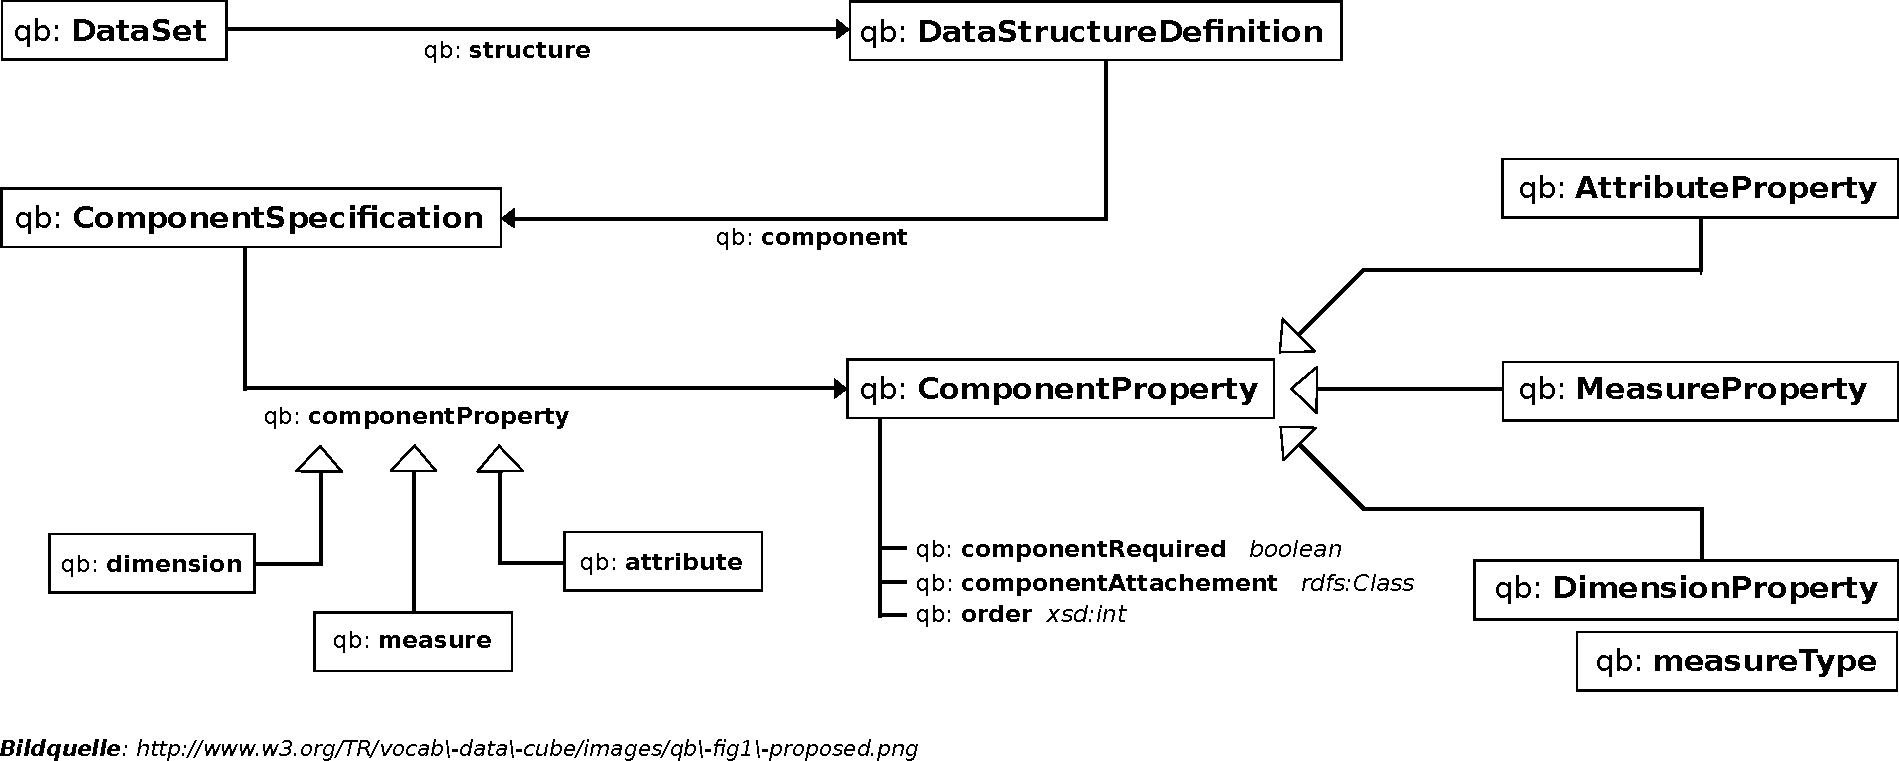
\includegraphics[width=15cm]{DataCube/DataCubeVocabulary_Figure_CS_DimMeaAttr.pdf}
    \caption{Für Komponenten relevanter Ausschnitt der Zusammenfassung aus dem DataCube Vokabular.}
    \label{fig:DataCubeVocabulary_Figure_CS_DimMeaAttr}
\end{figure}

Jeder Datensatz eine zugehörige Datenstruktur-Definition, welche die Beobachtungspunkte innerhalb des Datensatzes näher definiert. Dazu besitzt diese Datenstruktur-Definition Verbindungen zu allen nötigen Ressourcen, die die Struktur und Semantik des Datensatzes und seiner Inhalte klar beschreiben.

\newpage
\noindent
Mit der Datenstruktur-Definition sind die Dimensionen, Messwerte und Maßeinheiten jedoch nicht direkt verbunden, sondern zwischen ihnen befinden sich noch die Komponentenspezifikationen. Dabei ist jeder Komponentenspezifikation genau eine Komponente zugeordnet, wobei eine Komponente entweder vom Typ\com{Dimension-, \\ Measure- und \\ Attribute-\\Property} \textit{DimensionProperty}, \textit{MeasureProperty} oder \textit{AttributeProperty} ist. Diese Properties wiederum sind allesamt von \textit{ComponentProperty} abgeleitet. Die Beobachtungspunkte verwenden später nur die URI der Komponenten und nicht die der zugehörigen Komponentenspezifikationen. Wenn im Folgenden von einer Dimension bzw. Messwert oder Maßeinheit die Rede ist, sind damit sowohl die Komponente selber als auch die zugehörige Komponentenspezifikation gemeint. 

Die Abbildung \ref{fig:DataCubeVocabulary_Figure_CS_DimMeaAttr} zeigt eine Übersicht, welche die Zusammenhänge zwischen den einzelnen Elementen, die zur Definition des Datensatzes benötigt werden, illustriert.


%
% ----------------------------------------------------------------------------------
%
% SS
%
\newpage
\section{CubeViz: Ein facettierter Browser für Statistiken}
\label{sec:chapterCubeViz}

CubeViz\footnote{\url{http://aksw.org/Projects/CubeViz.html}} ist eine Software zur Visualisierung von statistischen Daten, die auf dem DataCube-Vokabular basieren. Sie ist dabei als Komponente für das semantische Content-Management-System OntoWiki entwickelt und bietet dem Benutzer die Möglichkeit, über sogenannte Facetten seinen Fokus auf die vorliegenden Daten zu konfigurieren. Das bedeutet, dass er über das Setzen von Filtern und Einstellungen sowohl die Datenauswahl als auch die Visualisierung anpassen kann. \cite[S. 6]{CUBEVIZ-VISZSTATS} \cite[S. 5-6]{CUBEVIZ-PUBSTATIS}

An dieser Stelle soll kurz erläutert werden, warum CubeViz als Grundlage dieser Arbeit ausgewählt wurde. Zum Zeitpunkt der Erstellung der Arbeit stellte sich CubeViz als adäquater Browser für DataCube-Daten heraus. Ein weiterer Grund ist, dass der Autor bereits praktische Erfahrungen und inhaltliche Einsichten in CubeViz besaß. Die folgende Liste beinhaltet die Aspekte von CubeViz in der Version 0.9, die im Rahmen dieser Arbeit nötig sind:

\begin{itemize}
\setlength{\itemsep}{0mm}
    \item \nameref{sec:chapterCVRelatedPaper} (\ref{sec:chapterCVRelatedPaper})
    \item \nameref{sec:chapterCVUseCases} (\ref{sec:chapterCVUseCases})
    \item \nameref{sec:chapterCVArchiUI} (\ref{sec:chapterCVArchiUI})
    \item \nameref{sec:chapterCVFacetedDataSel} (\ref{sec:chapterCVFacetedDataSel})
    \item \nameref{sec:chapterCVDataUIHash} (\ref{sec:chapterCVDataUIHash})
    \item \nameref{sec:chapterCubeVizAsLinkedDataMashup} (\ref{sec:chapterCubeVizAsLinkedDataMashup})
\end{itemize}

\noindent
Der Fokus in den Ausführungen liegt dabei in auf Einordnung der einzelnen Elemente und welche Ausgangsbasis sie für die spätere Implementierung bereitstellen, denn CubeViz bietet bereits eine Reihe wichtiger Funktionen. Das Kapitel beschreibt also die Ausgangssituation und stellt somit eine Ist-Analyse dar.

\noindent
Es gibt bereits eine wissenschaftliche Veröffentlichung für das \textit{Semantic Web Journal}, in welcher aufgearbeitete Teile dieses und anderer Kapitel enthalten sind. Sie ist zum Zeitpunkt der Fertigstellung dieser Arbeit noch in der Begutachtung, liegt aber bereits als Referenz \cite{CUBEVIZ-FUTUREPAPER} vor.


%
% SSS
%
\subsubsection{Kurzüberblick von TypeScript}
\label{sec:chapterCVTypeScript}

Dieses Unterkapitel soll einen kurzen Abriss zu der Sprache \textit{TypeScript}\footnote{\url{http://typescriptlang.org}} geben, weil sie das Fundament für die Benutzeroberfläche von CubeViz bildet. TypeScript ist eine von Microsoft entwickelte Skriptsprache, um fehlende Spracheigenschaften und Funktionalitäten von JavaScript zu ergänzen. Sie besitzt nun statische Typisierung sowie eine viel umfangreichere Unterstützung von Objektorientierter Programmierung. 

\newpage
\noindent
Bei der Planung wurde darauf geachtet, dass TypeScript die Entwicklung komplexer Softwareprojekte und die Zusammenarbeit großer Teams unterstützt. \cite[S. 1, 8 und 10]{TYPESCRIPT-SPEC} Aufgrund dieser Features entschieden sich die Entwickler von CubeViz für eine Implementierung von CubeViz in TypeScript. Damit war eine stabile Basis geschaffen und die Nutzung von skalierbaren Entwicklungsmethoden gegeben.



%
% SS
%
\subsection{Verwandten Arbeiten über die Visualisierung statistischer Daten}
\label{sec:chapterCVRelatedPaper}

Es folgt die Vorstellung einer Reihe von veröffentlichten Papern, die sich mit dem Thema der Visualisierung statistischer Daten befassen.

\begin{itemize}    
    \item \textit{Publishing Statistical Data on the Web} -- Hierbei geht es um die Frage, in welcher Form statistische Daten im Internet verwaltet werden können. In dem Zusammenhang werden die zwei Ansätze \textit{OLAP2DataCube} und \textit{CSV2DataCube} vorgestellt, die beschreiben, wie man statistische Daten explorieren und veröffentlichen kann. In diesem Paper wird CubeViz zur Visualisierung der statistischen Daten eingesetzt. Dabei wurde die erste Version von CubeViz genutzt, welche Tom-Michael Hesse in seiner Masterarbeit entwickelt hat. \cite{CUBEVIZ-PUBSTATIS}   
    
    \item \textit{Linked Open Data Statistics: Collection and Exploitation} -- Dieses Paper stellt eine Demo-Version mit LODStats\footnote{\url{http://aksw.org/Projects/LODStats.html}} vor, mit welcher man Open Linked Data Statistiken sammeln und explorieren kann. Es werden sowohl interne Abläufe in der Anwendung als auch die Benutzeroberfläche zur Exploration von Daten vorgestellt. Am Ende wird die Visualisierung der statistischen Daten mithilfe von CubeViz beschrieben. \cite{CUBEVIZ-VISZSTATS}     
    
    \item \textit{OntoWiki - An Authoring, Publication and Visualization Interface for the Data Web} -- Das Paper behandelt vordergründig die Software OntoWiki und beschreibt, wie dessen Funktionen die Verwaltung und Exploration großer statistischer Datensätze unterstützt. Es werden umfangreiche Anwendungsfälle aus den Bereichen der Datenintegration in Unternehmen, Daten aus der öffentlichen Verwaltung sowie den Digitalen Geisteswissenschaften (digital humanities) beschrieben. CubeViz übernimmt auch dort wieder die Visualisierung und Teile der Exploration von statistischen RDF-Daten. \cite{ONTOW-DATAWEB}
    
    \item \textit{Towards Next Generation Health Data Exploration: A Data Cube-based Investigation into Population Statistics for Tobacco} -- Die Autoren des Papers entwickelten ein Werkzeug namens \textit{qb.js}\footnote{\url{http://orion.tw.rpi.edu/~jimmccusker/qb.js}}, welches Nicht-Spezialisten einen Zugang zu statistischen Daten ermöglichen soll. Basierend auf dem DataCube-Vokabular werden an späterer Stelle Visualisierungen bereitgestellt. Ebenso wie CubeViz, exploriert man die Daten über eine Facetten-orientierte Suche. Dieses Paper stellt einen alternativen Ansatz zur Exploration und Visualisierung von DataCube-basierten Daten bereit.\cite{CUBEVIZ-ALTERAPPR}

\end{itemize}


%
% SS
%
\subsection{Unterstützte Anwendungsfälle}
\label{sec:chapterCVUseCases}

In der Einleitung wurden die für diese Arbeit wichtigen Anwendungsfälle bereits kurz erläutert (siehe Kapitel \ref{sec:chapterUseCaseList}).\com{Kapitel \ref{sec:chapterUseCaseList}, S. \pageref{sec:chapterUseCaseList}} Die bisherigen Fakten werden nun um technische Informationen ergänzt. 

%
% SSS
%
\subsubsection{Exploration statistischer RDF-Daten}
\label{sec:chapterUC1}

Der Anwendungsfall \nameref{sec:chapterUC1} ist teilweise im Themengebiet der \textit{explorativen Datenanalyse} angesiedelt. Sie ist ein Teilgebiet der Statistik und wurde von John W. Tukey im Rahmen einer Arbeit aus dem Jahre 1977 eingeführt. Er schlug vor, statistische Daten zur Formulierung eigener Hypothesen zu verwenden, um sie dann später unter Verwendung dieser Daten zu testen.\cite{EXPLORE-STAT} 

Die Software CubeViz unterstützt den Benutzer dabei in Form eines Browsers, der eine Facetten-orientierte Exploration ermöglicht. Bei der Facetten-orientierten Exploration wird über die Konfiguration der Meta-Daten die dargestellte Menge an Beobachtungspunkten verändert. Basierend darauf werden dann eine Reihe von Visualisierungen angeboten. So erhält der Benutzer unterschiedliche Blickwinkel auf die gleichen Daten.

%
% SSS
%
\subsubsection{Kollaboratives Explorieren und Bearbeiten von statistischen RDF-Daten}
\label{sec:chapterUC2}

Beim zweiten Anwendungsfall liegt der Fokus darauf, dass der Autor einer wissenschaftlichen Publikation für seine statistischen Daten mithilfe von CubeViz eine Reihe von Sichten (Visualisierungen) definiert. Stellt er diese Links später seinen Lesern bereit, so erhalten diese die Möglichkeit, die Daten moderiert zu explorieren. Diese Links referenzieren eine konkrete Konfiguration einer Visualisierung eines definierten Datenausschnittes (siehe Kapitel \ref{sec:chapterCVDataUIHash}).\com{Kapitel \ref{sec:chapterCVDataUIHash} \\ S. \pageref{sec:chapterCVDataUIHash}} CubeViz erlaubt es, dass jeder Leser selbst auch eigene Sichten definieren kann oder sogar die Werte im beschränkten Rahmen verändert, um sie dann dem Autor wieder zur Verfügung zu stellen. Auf diese Weise soll eine Diskussion über Hypothesen basierend auf den statistischen Daten entstehen können.

%
% SSS
%
\subsubsection{Vergleich von zwei Datensätzen}
\label{sec:chapterUC3}

Im dritten und letzten Fall geht es um den \nameref{sec:chapterUC3}. Im Vergleich werden die Beobachtungen aus den Datensätze unter gemeinsamen Gesichtspunkten betrachtet. CubeViz wird dabei für die Konfiguration der Meta-Daten genutzt, um damit die Menge der Beobachtungen zu definieren. Daraufhin sollen Vergleiche der Meta-Daten selbst oder zwischen den Werten der einzelnen Beobachtungspunkte möglich sein. CubeViz bietet dabei den Zugang auf verschiedenen Ebenen an, mit dem Ziel, Hypothesen zu bestätigen bzw. zu widerlegen oder neue aufzustellen. 


\newpage 
\noindent

Dieser Anwendungsfall wird von CubeViz nur sehr unzureichend unterstützt. So muss man beispielsweise CubeViz mindestens in zwei getrennten Browser-Tabs geöffnet haben, um jeweils einen Datensatz für den Vergleich auswählen zu können. Darauf wird an späterer Stelle nochmal eingegangen.




%
% SS
%
\subsection{Architektur von CubeViz}
\label{sec:chapterCVArchiUI}

Die Vorstellung von CubeViz beginnt mit dessen Benutzeroberfläche. Dies hat den Grund, dass der Großteil der Programmlogik auf der Client-Seite in Form von Java-Script-Code vorliegt. Das Backend, in PHP geschrieben, ist schlank gehalten und dient nur als eine Art Proxy zwischen der Benutzeroberfläche und der Datenbank.

%
% SSS
%
\subsubsection{Integration in OntoWiki}

Zu Beginn soll der Rahmen beschrieben werden, in dem die Benutzeroberfläche von CubeViz eingebunden ist: die Oberfläche von OntoWiki. Auf der Abbildung \ref{fig:OntoWiki_UserInterfaceRegions} ist die Einteilung der Benutzeroberfläche der Standardtheme \textit{silverblue} von OntoWiki illustriert. Im \textit{Kopfbereich} (gelb) befindet sich ein fester, von OntoWiki selbst definierter, Bereich, der das Hauptmenü beinhaltet. Darunter, auf der linken Seite, befindet sich die \textit{Sidebar} (blau). \\

%
% Abbildung
%
\begin{figure}[h!]
    \centering
    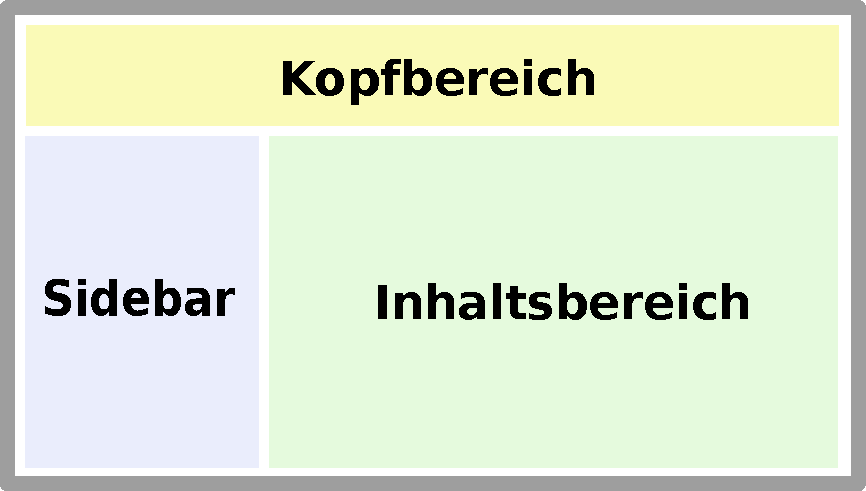
\includegraphics[width=5.5cm]{OntoWiki/UserInterfaceRegions.pdf}
    \caption{Grobe Einteilung der Benutzeroberfläche von OntoWiki (Standardtheme).}
    \label{fig:OntoWiki_UserInterfaceRegions}
\end{figure}

\noindent
Sie enthält von Komponenten registrierte Module und stellt sie dar. Module stellen in der Regel einfache Menüs und weiterführende Links für den Benutzer bereit. Zuletzt der \textit{Inhaltsbereich} (grün), welche den meisten Platz auf dem Bildschirm einnimmt. 

Dieser kann nochmals erweitert werden um Tabs und andere vordefinierte Oberflächenelemente. Es ist zwar möglich die Standardtheme von OntoWiki zu verändern oder gar eine komplett neue zu erstellen, jedoch wird im Folgenden die Standardtheme von OntoWiki in der Version 0.9.10\footnote{\url{https://github.com/AKSW/OntoWiki/tree/v0.9.10}} im Mittelpunkt stehen.

%
% Abbildung
%
\begin{figure}[h!]
    \centering
    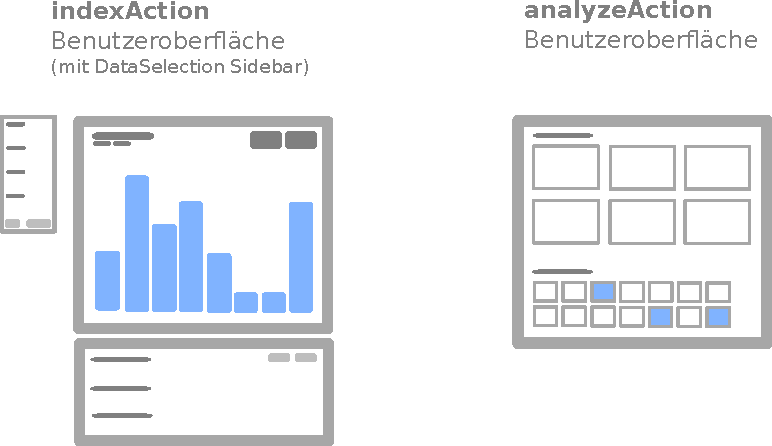
\includegraphics[width=9.6cm]{CubeViz/Overview.pdf}
    \caption{Einbindung von CubeViz in OntoWiki.}
    \label{fig:CubeViz_Overview}
\end{figure}

Die Abbildung \ref{fig:CubeViz_Overview} stellt die beiden Benutzeroberflächen von CubeViz gegenüber. Auf der linken Seite (indexAction) ist die Oberfläche zur Exploration von statistischen Datensätzen illustriert. Die Benutzeroberfläche daneben (analyzeAction) stellt den Analysebereich dar, über den der Benutzer einen ausgewählten statistischen Datensatz untersuchen kann.

Diese beiden Benutzeroberflächen integrieren sich direkt in die Standardtheme von OntoWiki und nutzen primär den Inhaltsbereich.


\newpage 
\noindent
Wird zudem ein Modell ausgewählt, welches DataCube-Informationen enthält, wird in der Sidebar ein weiteres Modul eingebunden. Dieses bietet dem Benutzer eine Maske zur Datenselektion an. 

OntoWiki baut bei der Strukturierung der Programmlogik und Präsentation auf dem MVC-Muster auf und nutzt dafür die jeweiligen Klassen aus dem Zend-Framework\footnote{\url{http://framework.zend.com}} in der Version 1.x. Daher basiert auch CubeViz auf diesem Architektur-Paradigma. CubeViz besitzt einen eigenen Controller, der die Eingaben des Benutzers sowohl der Benutzeroberfläche als auch über AJAX-Anfragen von den JavaScript-Bibliotheken verarbeitet und die beiden in Abbildung \ref{fig:CubeViz_Overview} dargestellten Benutzeroberflächen bereitstellt.

%
% SS
%
\subsubsection{Detaillierte Beschreibung der Architektur}

In diesem Teil wird auf die Architektur der Benutzeroberfläche und der dahinter liegenden Logik von CubeViz eingegangen. Das Ziel ist es, einen Überblick über die einzelnen Bestandteile sowie ihr Zusammenspiel zu erhalten. Wie bereits erwähnt, basiert die Komponente auf dem MVC-Muster, die Benutzeroberfläche hingegen verwendet eine Adaption davon, stark inspiriert von der genutzten Architektur in der \textit{Backbonejs-JavaScript-Bibliothek}\footnote{\url{http://backbonejs.org}}. \\

%
% Abbildung
%
\begin{figure}[h!]
    \centering
    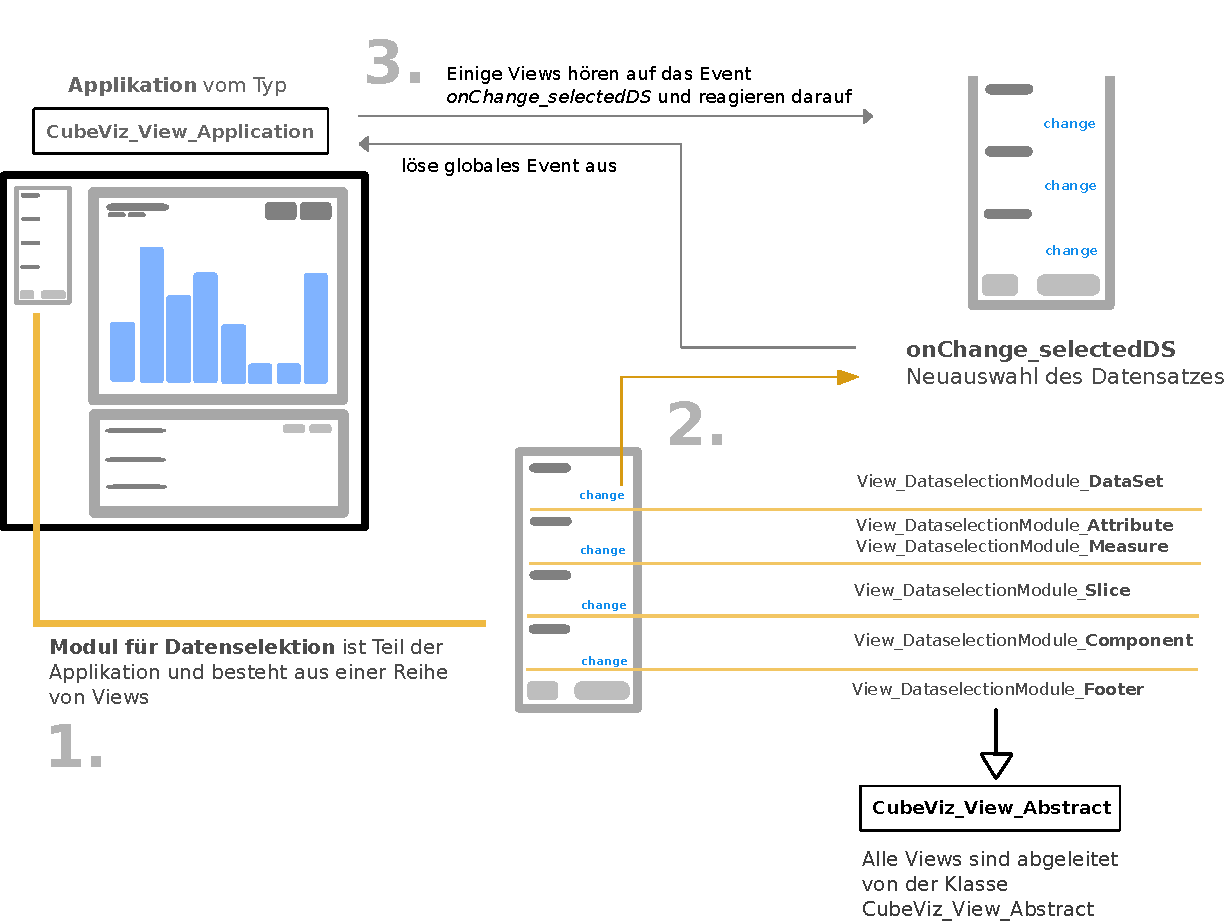
\includegraphics[width=15.5cm]{CubeViz/ApplicationViewInteraction.pdf}
    \caption{Illustration des Zusammenspiels zwischen Applikation und den Views.}
    \label{fig:CubeViz_ApplicationViewInteraction}
\end{figure}

\noindent
Ein Zitat\footnote{Zitat von \url{http://backbonejs.org/\#View}} auf der Projekthomepage beschreibt die Idee hinter der Architektur von Backbonejs-Anwendungen. So teilt man die Benutzeroberfläche in einzelne Teile auf, wobei jeder Teil durch einen \textit{View} repräsentiert wird, der sich um die Darstellung der Inhalte und die Interaktion mit dem Benutzer kümmert. Auf diese Weise kann man abgegrenzte Bereiche auf dem Bildschirm aktualisieren, ohne die gesamte Benutzeroberfläche neu zu laden. An einem View angedockt sind die sogenannten Modelle (\textit{Models}), welche die eigentliche Programmlogik beinhalten. CubeViz implementiert diese Architektur in Form einer zentralen Anwendungsinstanz, welche die Views verwaltet. Zusätzlich bietet sie ein View-übergreifendes Event-System, wodurch die Views untereinander auf Ereignisse reagieren können. 


\newpage 
\noindent
Diese Möglichkeit ist in Backbonejs nicht mittelbar gegeben. Es werden zwei Klassen dafür verwendet. Erstere Klasse heißt \verb|CubeViz_View_Application| und sie verwaltet alle Views und stellt eine Eventverwaltung bereit. Sie kann einerseits eine komplette Seite mit den jeweiligen Views repräsentieren, oder nur einen Seitenbereich. Letzteres bietet damit die Möglichkeit, logische Gruppen aus zusammengehörigen Views zu bilden. Die andere Klasse heißt \verb|CubeViz_View_Abstract| und von ihr ist jeder View abgeleitet. Diese stellt einige Hilfsfunktionen bereit, beispielsweise das Auslösen von globalen Events. (Zugehörige Illustration auf Abbildung \ref{fig:CubeViz_ApplicationViewInteraction})

Zusammenfassend lässt sich festhalten, dass die Benutzeroberfläche von CubeViz mithilfe von sogenannten Views strukturiert und verwaltet wird. Diese Views sind über die Anwendungsinstanz zu Gruppen zusammengefasst und können über diese untereinander kommunizieren. Das verwendete Konzept orientiert sich an dem MVC-Muster, wobei der Fokus auf dem View und dem Modell liegt, wobei der View auch einige Aufgaben des Controllers übernimmt.


%
% SS
%
\newpage
\subsubsection{Bestandteile der Benutzeroberfläche}
\label{sec:chapterCVUIParts}

CubeViz benutzt benutzt alle drei Bereiche der OntoWiki-Theme. Im Folgenden werden die einzelnen Oberflächenelemente dazu vorgestellt. In diesem Zusammenhang werden ebenfalls die Unzulänglichkeiten im Kontext dieser Arbeit erwähnt, welche zu späteren Veränderungen führten. Der Leser soll einerseits ein umfassendes Bild von CubeViz erhalten, aber andererseits auch etwas über dessen Schwächen erfahren.


%
% P
%
\paragraph{Linkes Seitenmenü}

%
% Abbildung
%
\begin{figure}[h!]
    \centering
    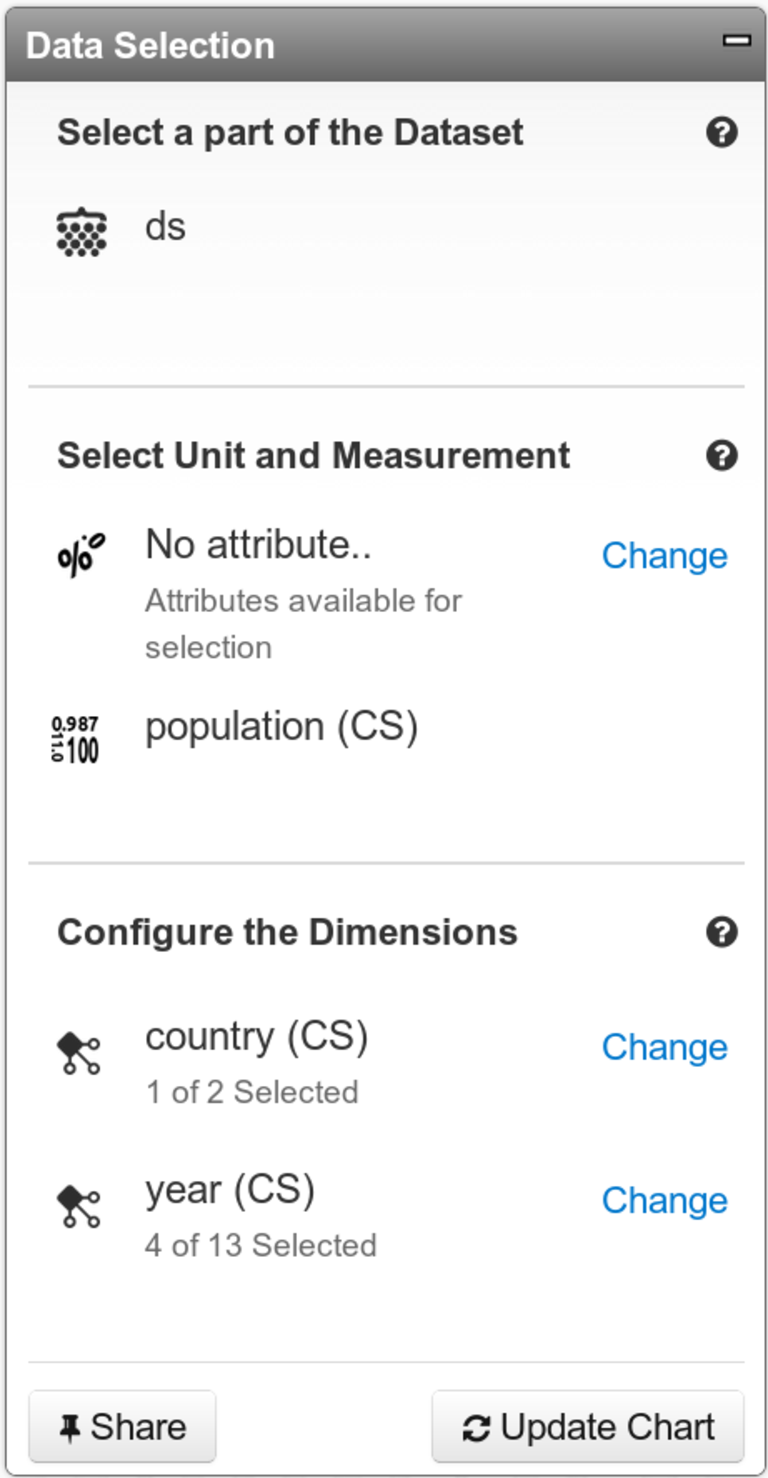
\includegraphics[width=4cm]{CubeViz/LeftSidebar.pdf}
    \caption{Benutzeroberfläche des Moduls zur Datenselektion und Facettierung.}
    \label{fig:CubeViz_LeftSidebar}
\end{figure}

In die Sidebar wird ein Modul integriert, welches genau dann angezeigt wird, wenn der Benutzer ein Modell mit gültigen DataCube-Informationen ausgewählt hat. Dieses Modul wird als \emph{linkes Seitenmenü}\com{Linkes \\Seitenmenü} bezeichnet und es ist der zentrale Anlaufpunkt zum Setzen von Facetten für die Exploration der statistischen Daten. Der Inhalt des Moduls basiert dabei auf dem ausgewählten Datensatz, wobei zu Beginn standardmäßig der erste Datensatz vorausgewählt wird. Auf der \mbox{Abbildung \ref{fig:CubeViz_LeftSidebar}} ist ein Screenshot davon zu sehen. Ganz oben befindet sich die Datensatz-Auswahl, welche die beiden Buchstaben \emph{ds} enthält. Es gibt jedoch keine Möglichkeit, diese zu verändern, denn CubeViz ist so eingestellt, dass es in diesem Modul eine Alternativauswahl unterdrückt, falls nur ein Element zur Auswahl steht. Nach der Datensatz-Auswahl folgt unmittelbar die Schnitt-Auswahl. Sie ist jedoch auf der Abbildung nicht sichtbar, weil der Beispieldatensatz keine Schnitte enthält. Gibt es Schnitte in einem ausgewählten Datensatz, so können diese hier spezifiziert werden. Unter dem obigen Block befindet sich der Block zur Konfiguration der Attribute und Messwerte. Auf der Abbildung kann man einen blauen Link mit der Aufschrift \emph{change} erkennen. Dazu gleich mehr. An vorletzter Stelle befindet sich der Dimensionsbereich, in dem die Dimensionen reihenweise aufgelistet werden. 


\newpage 
\noindent
Im Fußbereich findet man zwei Schaltflächen: Die mit \emph{Share} beschriftete Schaltfläche bietet das Verteilen eines Links ähnlich wie bei Facebook an, die andere ist mit \emph{Update Chart} beschriftet und führt zu dem Explorations- und Visualisierungsbereich.

Klickt man auf einen der oben erwähnten \emph{Change} Links, so sieht man einen ähnlichen Dialog wie auf  Abbildung \ref{fig:CubeViz_DimensionElementDialog} abgebildet. In diesem hat man die Möglichkeit, das  Element zu konfigurieren, zu dem der Link gehört. Im oberen Bereich ist der Titel und wenn vorhanden, der Beschreibungstext, des Elements eingeblendet. Darunter ist eine Reihe von Schaltflächen angebracht, welche zur Aus- und Abwahl der Elemente sowie zu deren Sortierung genutzt werden können. Hat man seine Anpassung vorgenommen, klickt man rechts unten auf die Schaltfläche \emph{Update Selection} oder bricht ohne Änderungen ab mit Klick auf die \emph{Cancel} Schaltfläche. \\

%
% Abbildung
%
\begin{figure}[h!]
    \centering
    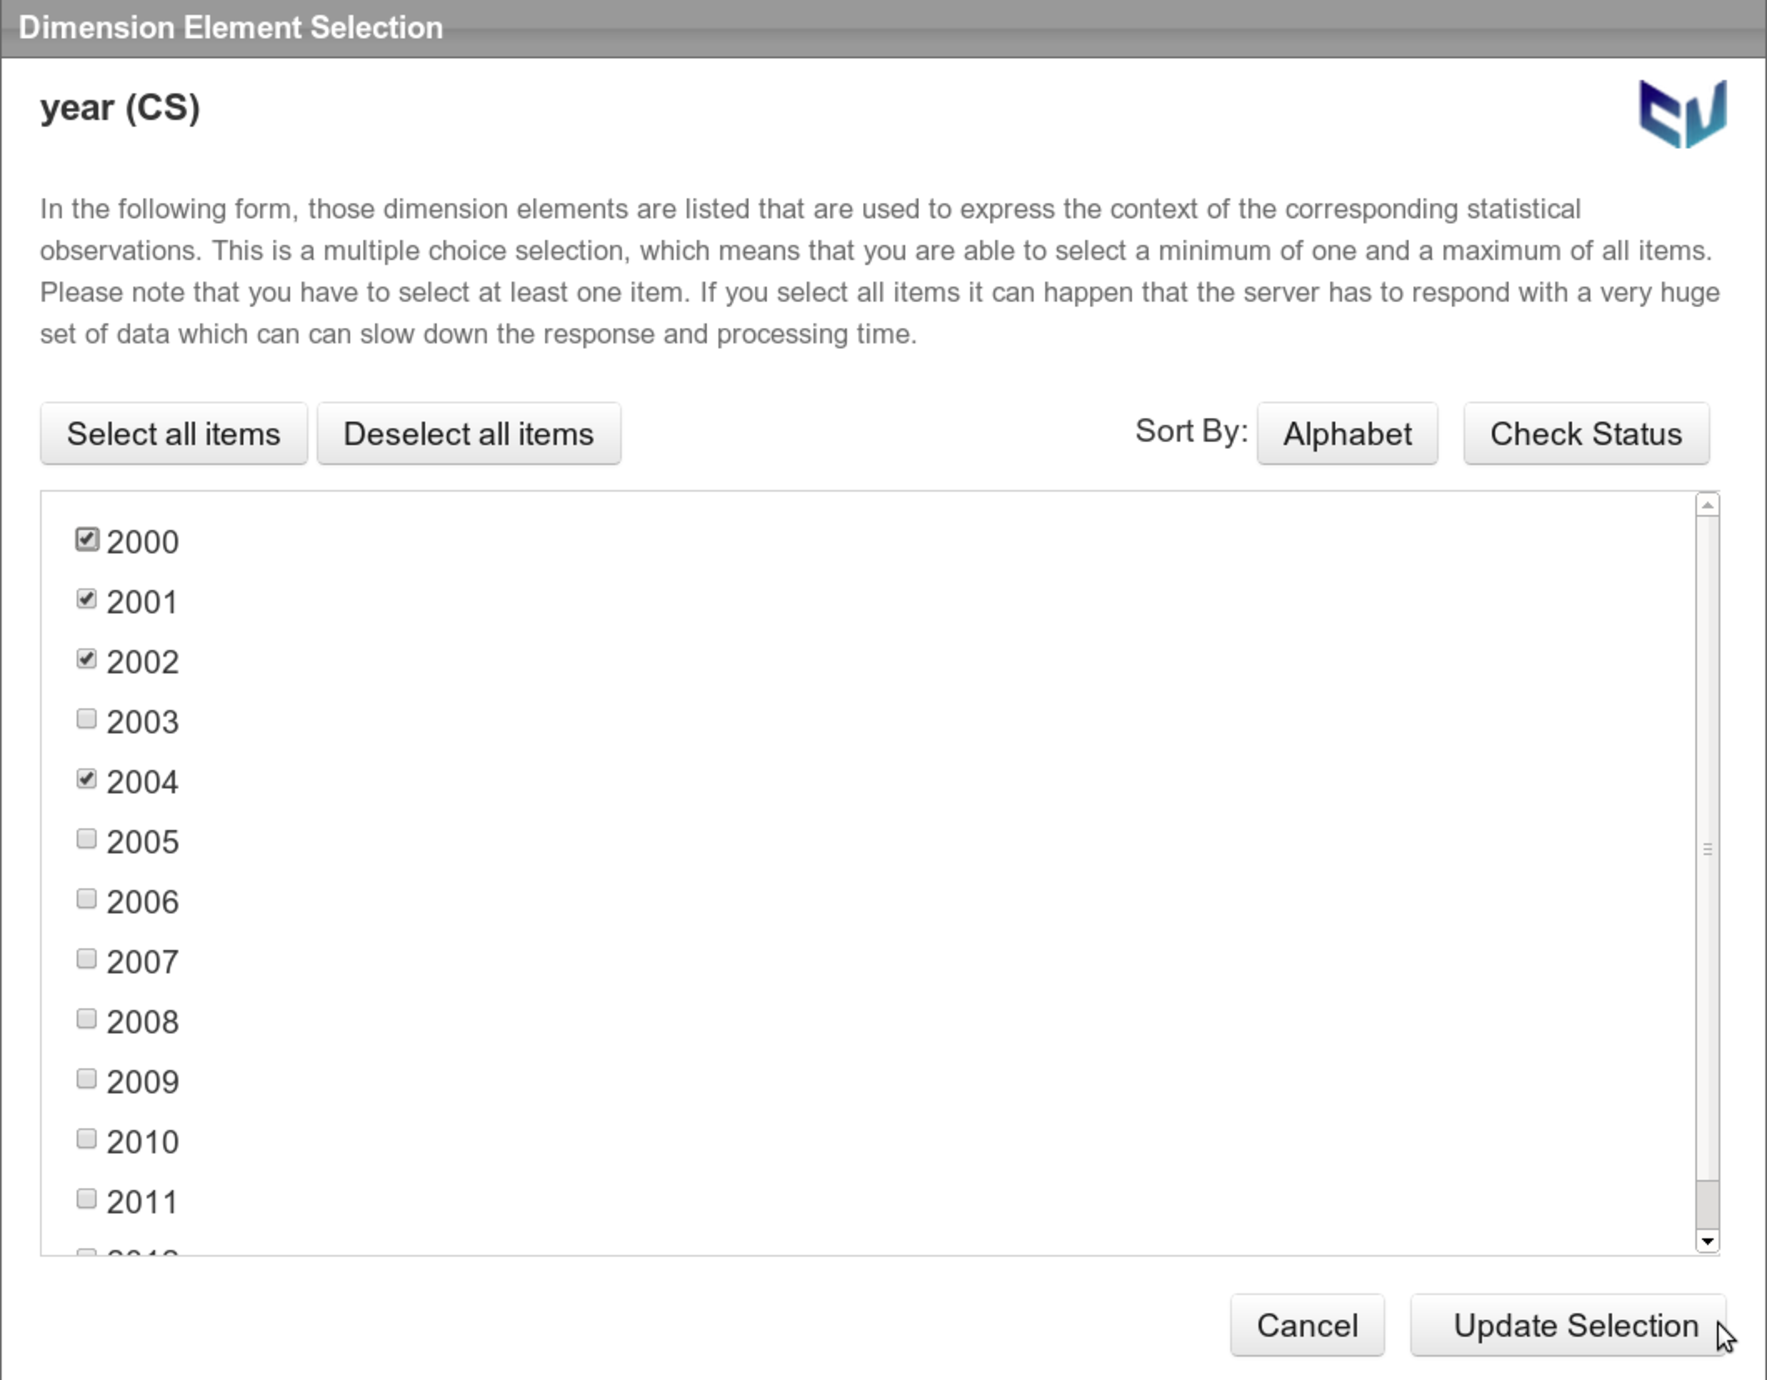
\includegraphics[width=11.4cm]{CubeViz/DimensionElementDialog.pdf}
    \caption{Benutzeroberfläche zur Facettierung eines konkreten Elements.}
    \label{fig:CubeViz_DimensionElementDialog}
\end{figure}

\noindent
Dieser Dialog nimmt eine zentrale Rolle bei der Facetten-orientierten Suche ein. Wie bereits erwähnt, kann man mithilfe von CubeViz statistische Daten über das Setzen von Facetten selektieren und aussortieren. Eine Facette entspricht dabei der Auswahl eines oder mehrerer Elemente in einer dieser Listen wie diesem Dialog. Einmal wählt man zwischen verschiedenen disjunkten Messwerten, ein andermal stellt man sich eine Gruppe von Dimensionselementen einer bestimmten Dimension\com{Kapitel \ref{sec:chapterCVFacetedDataSel} \\ S. \pageref{sec:chapterCVFacetedDataSel}} zusammen. Näheres zur Facetten-orientierten Datenselektion in Kapitel \ref{sec:chapterCVFacetedDataSel}.


%
% SSS
%
\paragraph{Explorations- und Visualisierungsbereich}

Den meisten Raum nimmt der Programmteil zur Exploration und Visualisierung von statistischen Daten ein (siehe Illustration auf Abbildung \ref{fig:CubeViz_UserInterfaceAreas}). Dieser nutzt ausschließlich den Inhaltsbereich der OntoWiki-Theme. 


\newpage 
\noindent
Zugänglich wird dieser aber erst, wenn man entweder über das bereits vorgestellte Modul zur Datenselektion eine Auswahl trifft, oder man den Programmteil mit gewissen Parametern direkt aufruft.

Beginnen wir mit dem \emph{Kopfbereich}.\com{Kopfbereich} Dieser dient dazu, allgemeine Informationen über das ausgewählte Modell sowie den Datensatz bereitzustellen. Daher findet man neben dem Titel des ausgewählten Modells und Datensatzes auch einen Link, der ein weiteres Fenster öffnet, in dem man weiterführende Informationen zu dem ausgewählten Modell findet. Rechts von dem Kopfbereich befindet sich der \emph{Visualisierungsselektor}.\com{Visualisie- rungs-\\ selektor} Über diesen hat der Benutzer die Möglichkeit, die Art der Visualisierung auszuwählen und danach entsprechend zu konfigurieren. Auf der Abbildung \ref{fig:CubeViz_ViszSelector} sieht man den Visualisierungsselektor und das zu einer Visualisierung zugehörige Konfigurationsmenü. \\

%
% Abbildung
%
\begin{figure}[h!]
    \centering
    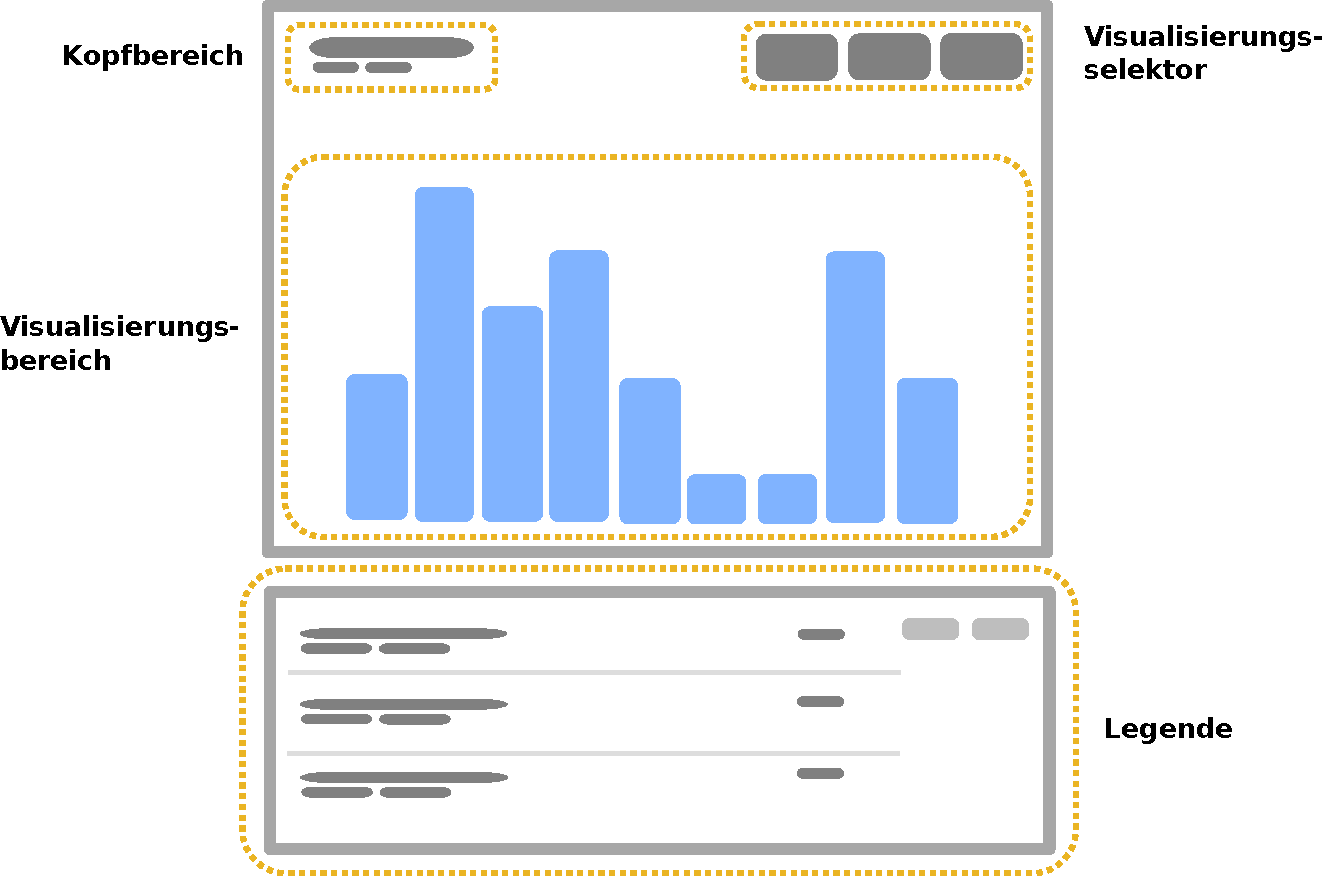
\includegraphics[width=13.5cm]{CubeViz/UserInterfaceAreas.pdf}
    \caption{Aufteilung der eigentlichen Benutzeroberfläche.}
    \label{fig:CubeViz_UserInterfaceAreas}
\end{figure}

\noindent
Die Aufgabe des Selektors ist es, dass man sich seine ausgewählten Daten in verschiedenen Visualisierungstypen darstellen lassen kann. Durch einen einfachen Klick auf das jeweilige Symbol wird die Visualisierung ausgewählt und angezeigt. Klickt man erneut darauf, so erscheint ein Menü zur Konfiguration der Visualisierung. Ein Beispiel dafür ist auf Abbildung \ref{fig:CubeViz_ViszSelector} zu sehen.

Das Menü \com{Kapitel \ref{sec:chapterCVDataUIHash} \\ S. \pageref{sec:chapterCVDataUIHash}} ist vordefiniert und dessen Erstellung wird in Kapitel \ref{sec:chapterCVDataUIHash} erläutert. Die Idee hinter diesem Selektor ist es, dass man durch mehrere Visualisierungen auch verschiedene Blickwinkel auf die Daten erhält. Man geht aber noch einen Schritt weiter und erlaubt dem Benutzer durch ein zusätzliches Konfigurationsmenü die ausgewählte Visualisierung weiter zu verändern. In diesem Bereich besteht sicherlich noch viel Potenzial zur Weiterentwicklung. 


%
% Abbildung
%
\begin{figure}[h!]
    \centering
    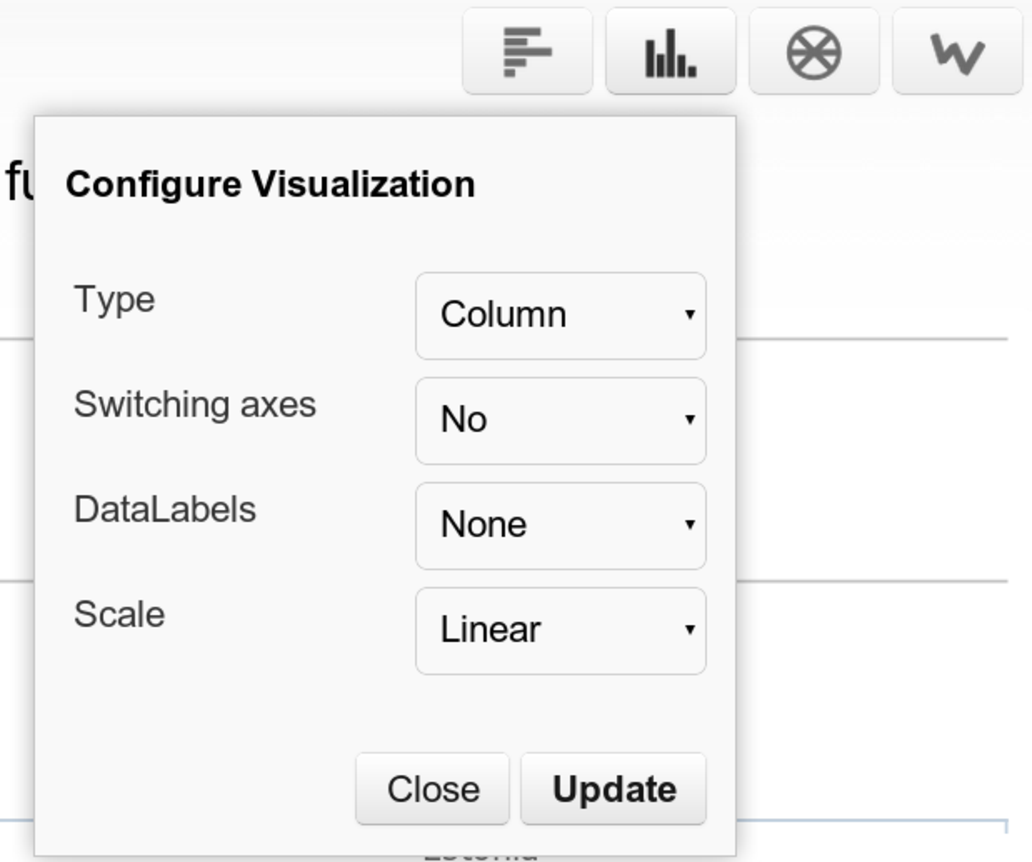
\includegraphics[width=7.5cm]{CubeViz/ViszSelector.pdf}
    \caption{Visualisierungsselektor mit vier Einträgen und ein Konfigurationmenü.}
    \label{fig:CubeViz_ViszSelector}
\end{figure}

\noindent
Der \textit{Visualisierungsbereich}\com{Visualisie-rungsbereich} ist von zentraler Bedeutung und nimmt daher den meisten Platz auf der Benutzeroberfläche in Anspruch. CubeViz nutzt für die Visualisierung der statistischen Daten ausschließlich die JavaScript Bibliothek namens \textit{HighCharts}\footnote{\url{http://www.highcharts.com/products/highcharts}}. Auf Abbildung \ref{fig:CubeViz_Visualization} ist ein Beispiel für eine Visualisierung dargestellt. Die Effizienz und Möglichkeiten des Dargestellten hängen direkt mit der genutzten Visualisierungsbibliothek ab. CubeViz kann daher nur indirekt die Visualisierung steuern.

%
% Abbildung
%
\begin{figure}[h!]
    \centering
    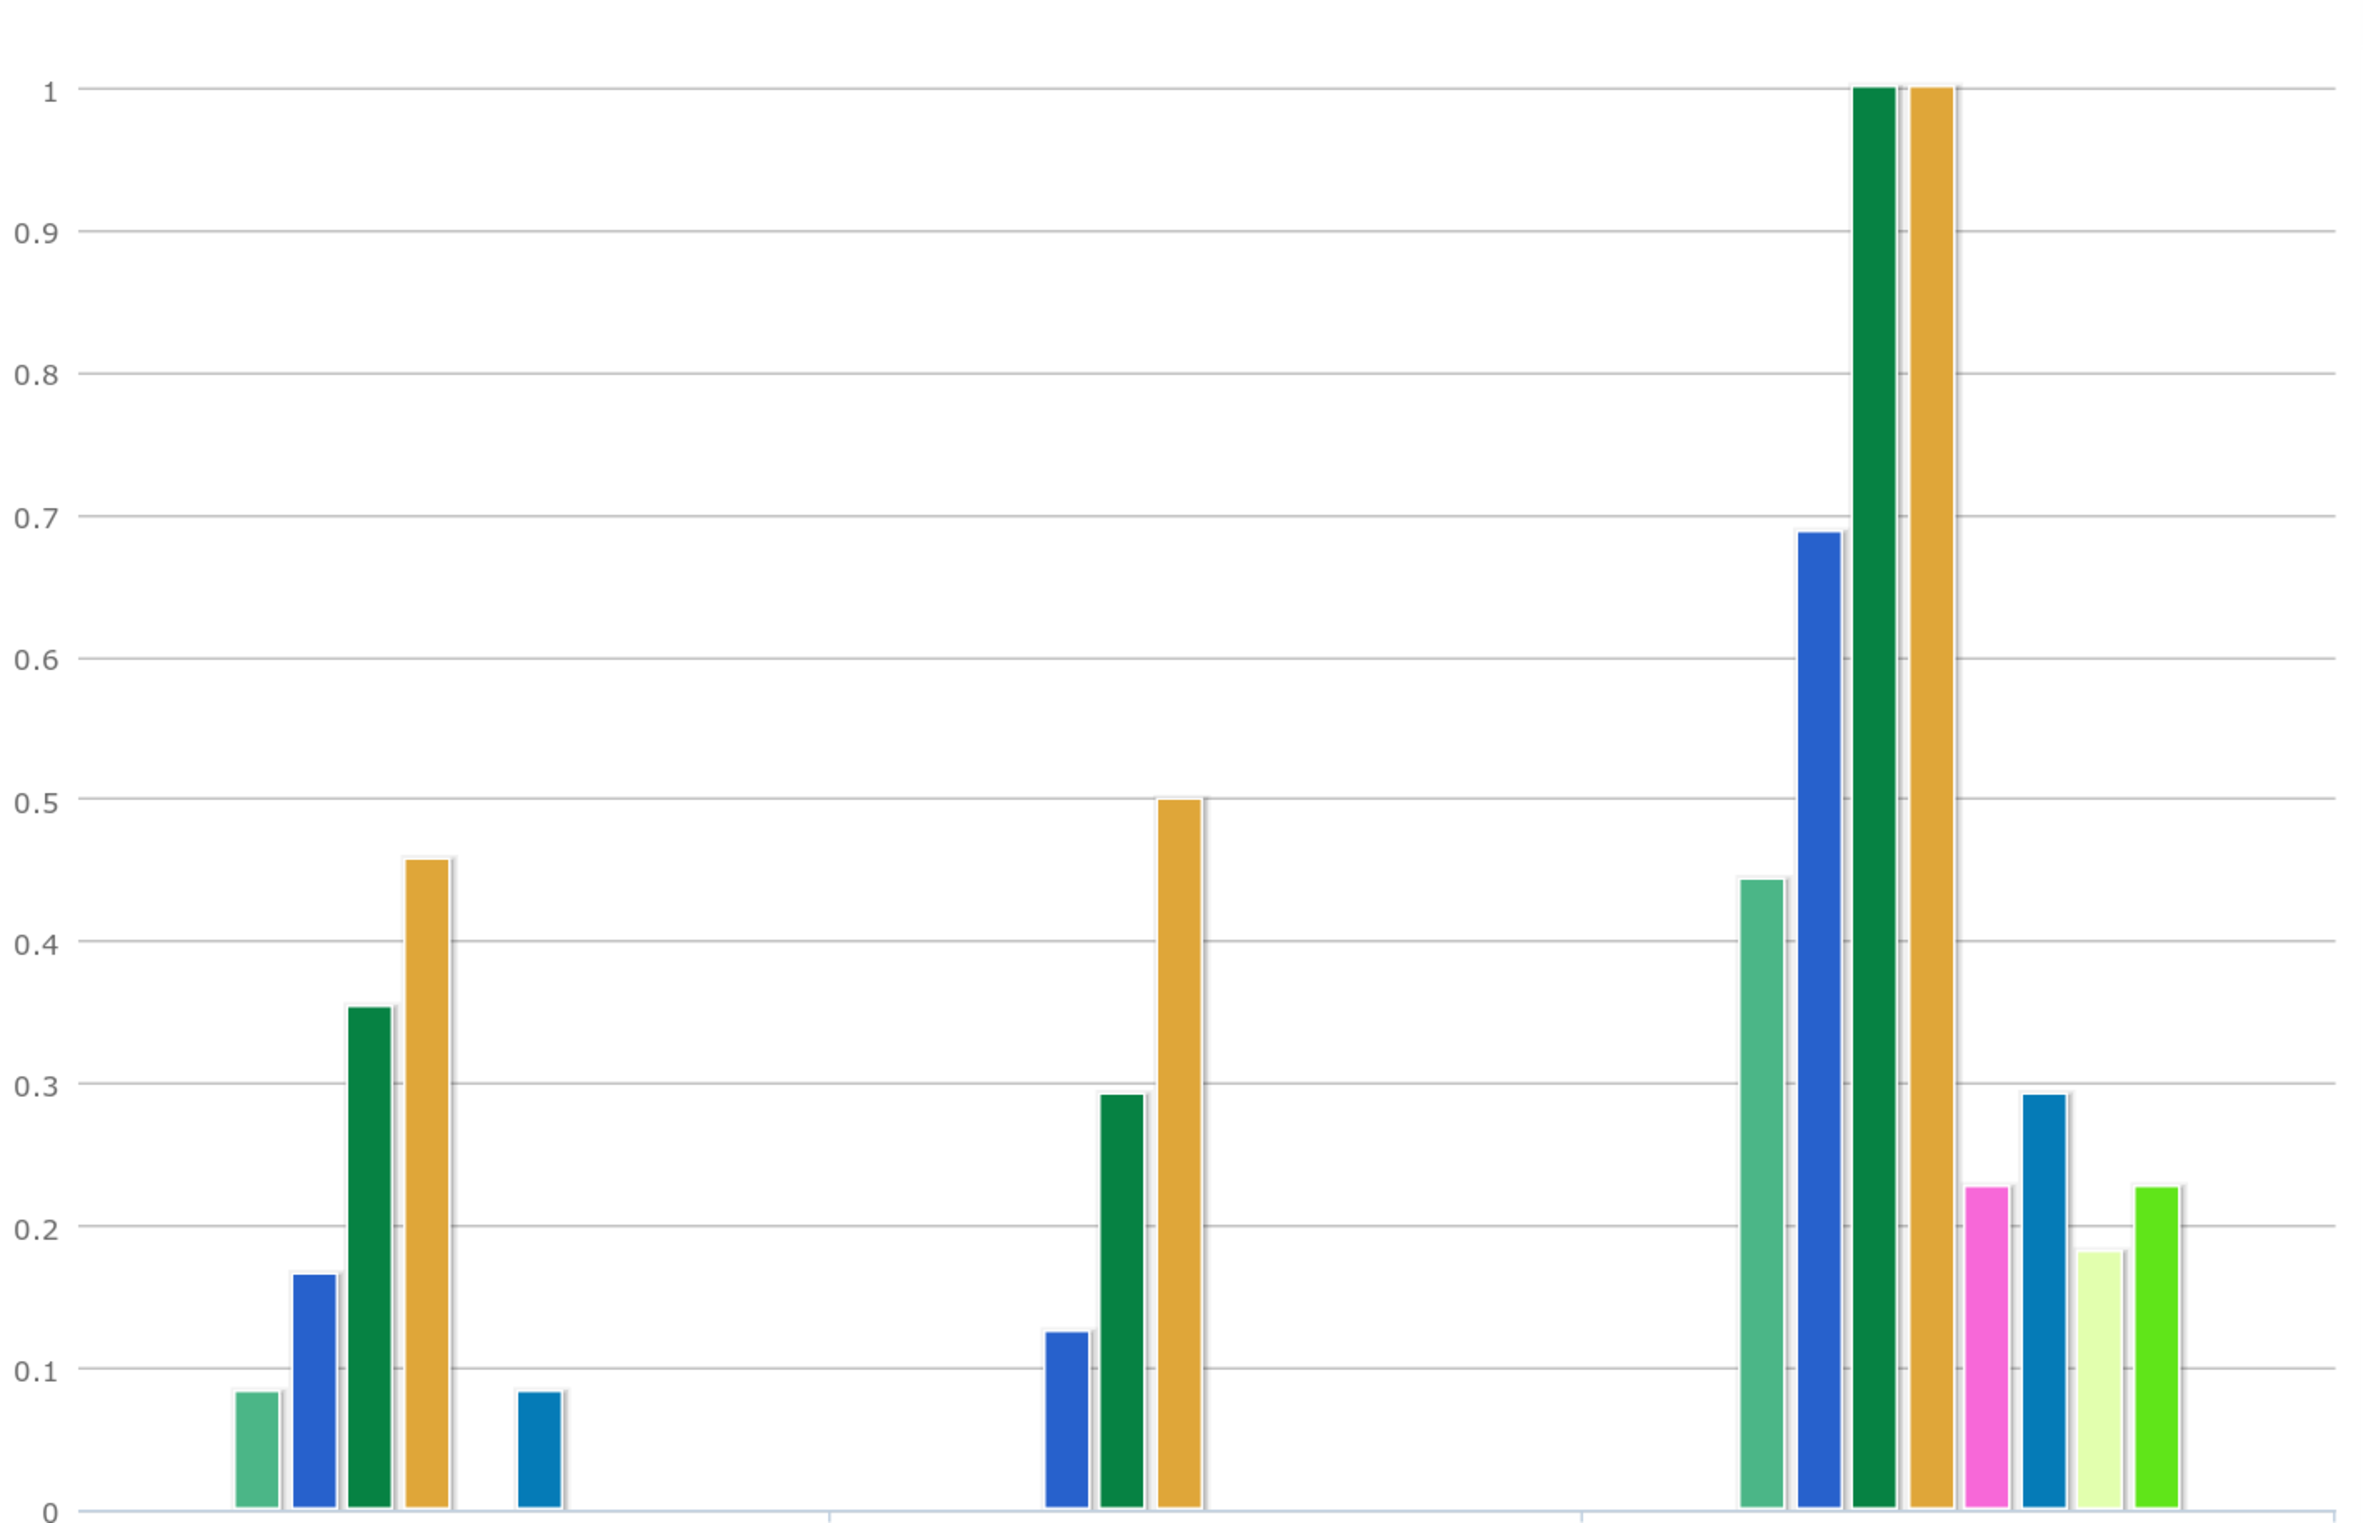
\includegraphics[width=8.8cm]{CubeViz/Visualization.pdf}
    \caption{Beispiel für ein Spaltendiagramm im Visualisierungsbereich.}
    \label{fig:CubeViz_Visualization}
\end{figure}


%
% Abbildung
%
\begin{figure}[h!]
    \centering
    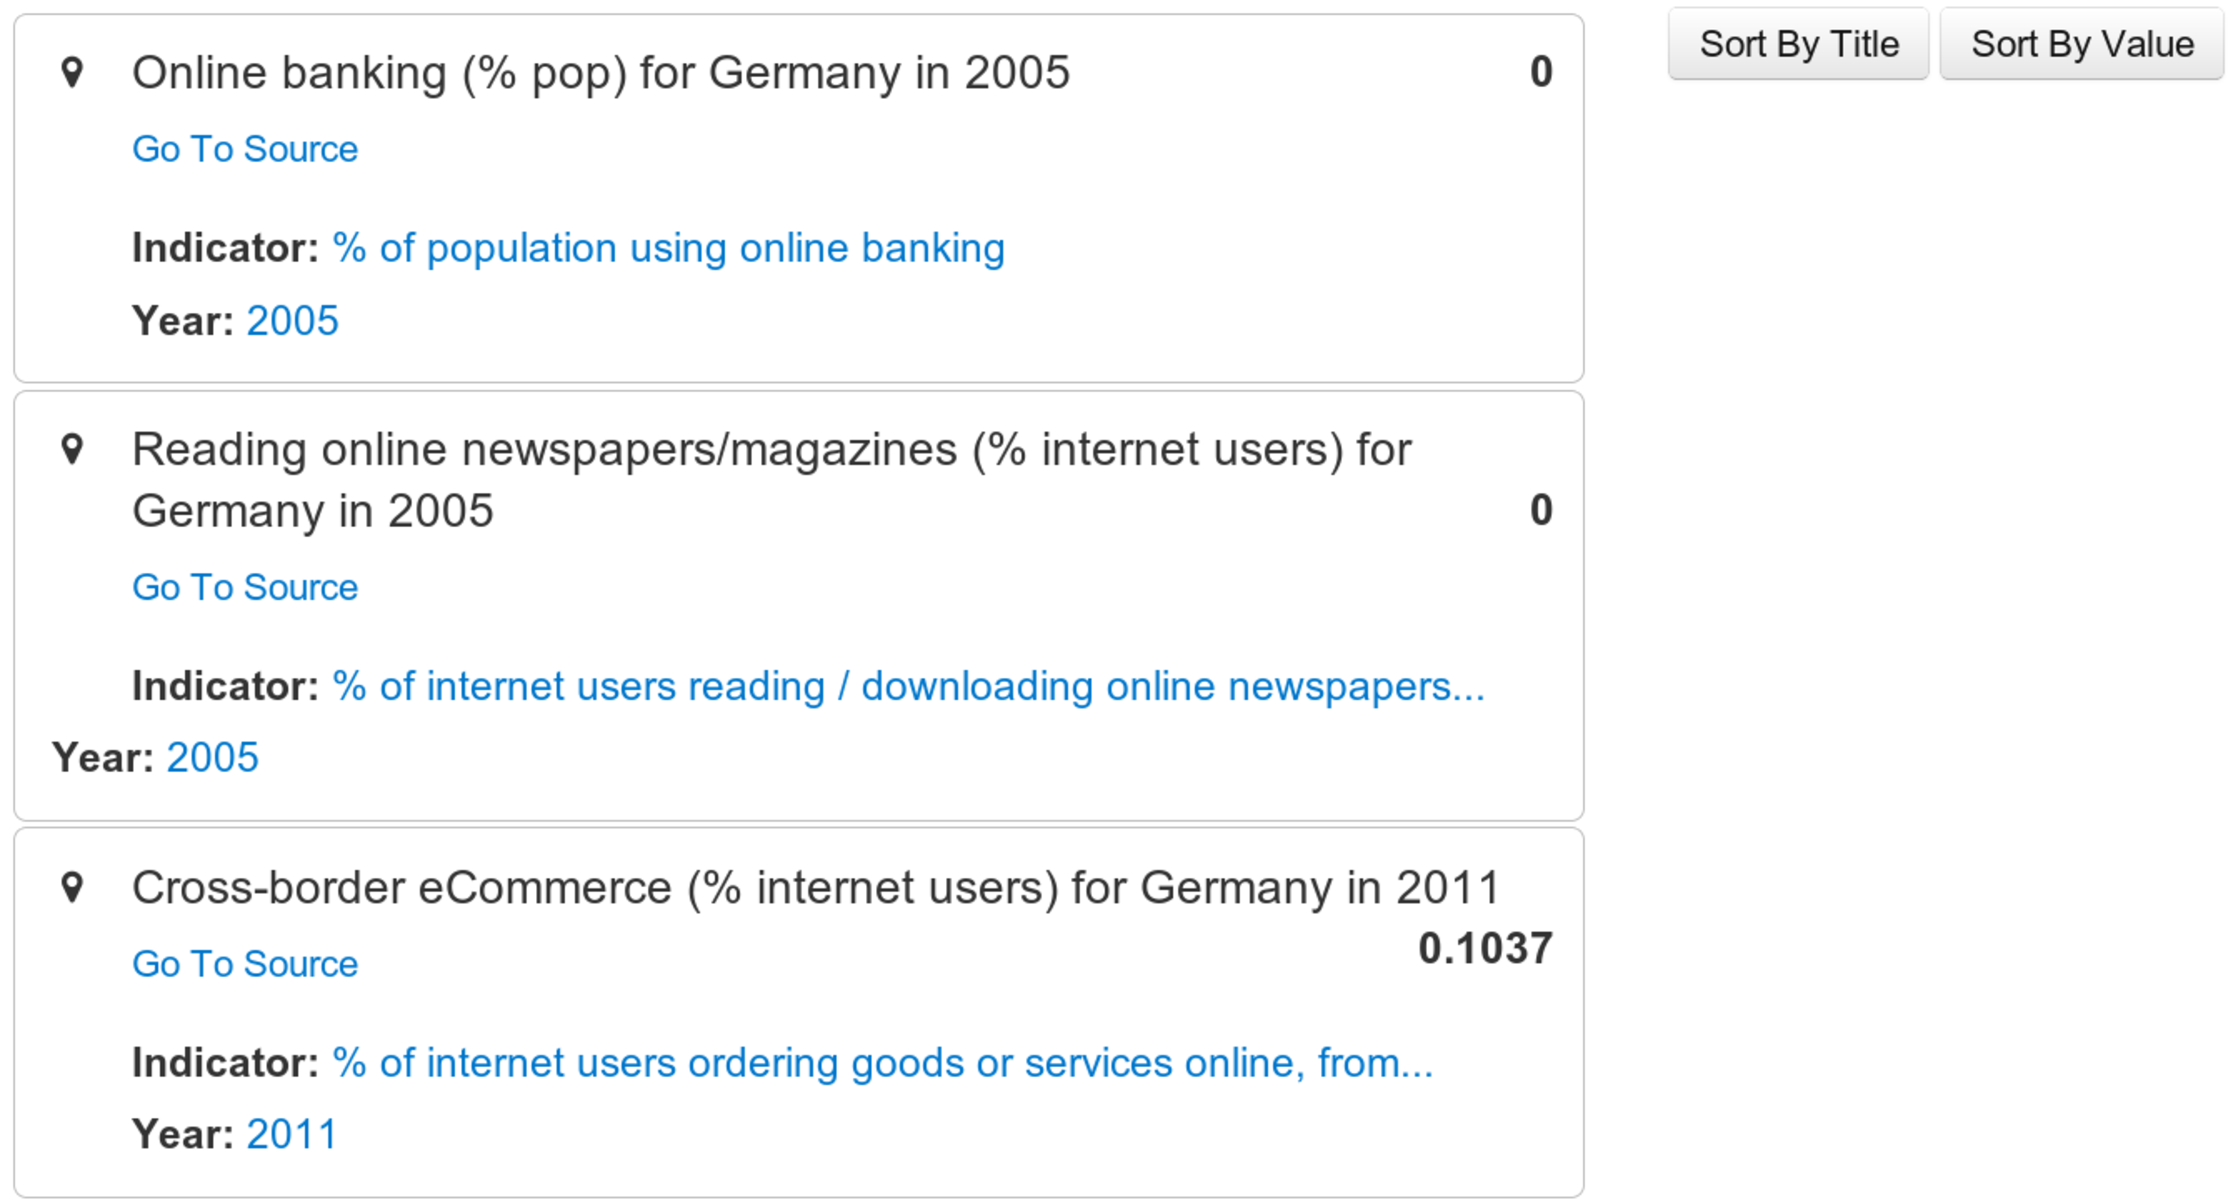
\includegraphics[width=15cm]{CubeViz/LegendObservations.pdf}
    \caption{Eine ausgeklappte Legende mit Beobachtungspunkten.}
    \label{fig:CubeViz_LegendObservations}
\end{figure}

\noindent
Zum Schluss soll nun die \textit{Legende} vorgestellt werden,\com{Legende} welche sich unter dem Visualisierungsbereich befindet und standardmäßig eingeklappt ist. Ihr Zweck ist die Auflistung der ausgewählten Beobachtungspunkte sowie die zu jedem Beobachtungspunkt gehörenden Dimensionselemente. Bei der Anzeige werden, wenn möglich, Hyperlinks verwendet, um dem Benutzer die Möglichkeit zu geben, direkt zu den Quelldaten zu springen. 

In der Liste der Beobachtungspunkte gibt es die Möglichkeit, eine alphabetische Sortierung nach Titel oder Messwert durchzuführen, wobei standardmäßig nach Titel sortiert wird. 

\newpage
\noindent
Auf der Abbildung \ref{fig:CubeViz_LegendObservations} ist ein Beispiel für eine ausgeklappte Legende mit drei Beobachtungspunkten zu sehen. Diese Beobachtungspunkte enthalten jeweils einen Link mit ihrer eigenen URL sowie Links zu ihren angebundenen Dimensionselementen. Auf der rechten Seite sieht man oben zwei Buttons, welche die Liste nach den Titeln der Beobachtungspunkte oder nach deren Messwerten aufsteigend sortiert.

In dieser Form fehlen der Legende eine Reihe von Dingen. \com{Anforderungen} So wäre eine viel feinere Sortierung wünschenswert, also eine auf- und absteigende Sortierung nach den jeweiligen Dimensionselementen eines Beobachtungspunktes (\textit{F-200})\label{req:F200source}\com{F-200, S. \pageref{req:F200}}. Besitzt der Beobachtungspunkt neben den bisher dargestellten Daten noch weitere, so sind diese in dieser Form nicht ersichtlich (\textit{F-210})\label{req:F210source}.\com{F-210, S. \pageref{req:F210}} 

Dies ist insbesondere bei dem Vergleich einzelner Beobachtungspunkte von Interesse, um z.B. zu erkennen, wo diese miteinander zusammenhängen. Gerade bei dem Vergleich der Beobachtungspunkte wäre es sehr hilfreich, wenn man deren jeweilige Messwerte\com{Anforderung \\ F-230, S. \pageref{req:F230}} zeitweilig anpassen könnte, um mit der Visualisierung \emph{herumspielen} zu können (\textit{F-230})\label{req:F230source}. Diese fehlenden Elemente werden als notwendig erachtet und sind auf der rechten Seite als Anforderungen referenziert.

%
% SS
%
\subsection{Die Facetten-orientierte Datenselektion}
\label{sec:chapterCVFacetedDataSel}

CubeViz bietet eine Facetten-orientiertes Datenselektion von DataCube-Elementen. Facetten-orientiert bedeutet, dass der Benutzer einen bestehenden Datenbestand über mehrere Filter einschränken kann, wobei jeder Filter dabei als Facette angesehen wird, über die man sich seiner gewünschten Ergebnismenge schrittweise annähert.\cite[S. 33]{FACETED-SEARCH}

\newpage
\noindent
Bei der Facettierung nimmt das Modul zur Datenselektion in der Seitenleiste die entscheidende Rolle ein. Darin kann man über eine Reihe von Dialogen die Auswahl der Daten auf verschiedene Art und Weise einschränken. Hauptausgangspunkt ist aber immer der ausgewählte Datensatz. Dieser wiederum setzt die Grenzen und Möglichkeiten bei der Anpassung und Auswahl der zugehörigen Elemente, wie der Maßeinheit oder den Dimensionen.


%
% SSS
%
\subsubsection{Vordefinierte Facetten als Einstieg in den DataCube}

Wie bereits erwähnt, kann man über die Definition von Schnitten\com{Schnitte \\ Datensatzfilter \\[0.2cm] 
\includegraphics[width=0.4cm]{semicon/slice2.pdf}} dem Benutzer besondere Beobachtungspunkte hervorheben. In CubeViz werden Schnitte anders kommuniziert, als im Vokabular vorgesehen, nämlich als Datensatzfilter, die den ausgewählten Datensatz einschränken. Wird ein solcher Filter ausgewählt, werden die jeweiligen Dimensionselemente vorausgewählt und der Benutzer hat dann keine Möglichkeit mehr. die entsprechenden Dimensionen zu verändern. CubeViz kann in der Version 0.9 nur mit Schnitten umgehen, die auf der Ebene der Dimensionselemente operieren. Über diesen Mechanismus erhält der Benutzer eine Möglichkeit, Facetten festzulegen, mit dem Unterschied, dass diese Art von Facetten vorher vom Betreuer des DataCube definiert wurden.


%
% SSS
%
\subsubsection{Datenselektion über Auswahl der Dimensionselemente}

Die wohl geläufigste Art eine bestimmte Menge an Beobachtungspunkten zu selektieren, ist über den Dialog zur Auswahl von Dimensionselementen (siehe Abbildung \ref{fig:CubeViz_DimensionElementDialog}). Dieser ist am unteren Ende des Moduls zur Datenselektion zu finden und er enthält eine Liste der Dimensionselemente, welche über eigene Schaltflächen aus- oder abgewählt werden können. Nach der Bestätigung der Selektion wird die entsprechende Menge an Beobachtungspunkte unmittelbar dargestellt und bei Bedarf kann hierher zurückkehrt werden, um weitere Anpassungen vorzunehmen. 


%
% SSS
%
\subsubsection{Facettierung über Messwert und Maßeinheit}

Man kann innerhalb eines Datensatzes mehrere Messwerte und Maßeinheiten definieren und die Beobachtungspunkte damit versehen. Auf diese Weise erhält man verschiedene Gruppen von Beobachtungspunkten, unterscheidbar anhand von Messwerten und Maßeinheiten. Da man im CubeViz nur einen Messwert zur gleichen Zeit verwenden kann, wird durch dessen Auswahl auch die Menge der Beobachtungspunkte eingeschränkt. Es werden alle Beobachtungspunkte aus der Menge entfernt, die den ausgewählten Messwert-Typ nicht besitzen. Auf diese Weise findet ebenfalls eine Art Facettierung statt. Bei den Maßeinheiten ist die Auswahl optional, jedoch schränkt eine Auswahl ebenfalls die Menge der Beobachtungspunkte ein.


%
% SS
%
\subsection{Speicherung der Datenselektion und Konfiguration der Visualisierung}
\label{sec:chapterCVDataUIHash}

CubeViz bietet die Möglichkeit, sowohl eine getroffene Datenselektion als auch visuelle Konfiguration zu speichern und später wieder zu benutzen. Dazu wird jeweils eine Datei im JSON-Format\footnote{\url{http://www.json.org}} angelegt, welche die nötigen JSON-Objekte abspeichert. Auf Abbildung \ref{fig:CubeViz_HashIllustration} wird dies skizziert.

In dem oberen Teil ist die Datenselektion\com{Daten-Hash} illustriert. An dieser Stelle ist ein Hash mit dem Präfix \verb|__cv_dataHash| dargestellt. Dieser Hash zeigt auf eine JSON-Datei, welche alle notwendigen Daten, wie den Datensatz, ausgewählte Dimensionen oder den Messwert beinhaltet. Durch die Speicherung dieser Informationen reduziert sich die Last für die Datenbank bei einem Wiederaufruf einer vorher gespeicherten Datenselektion teilweise erheblich, weil keine Datenbankabfragen mehr nötig sind. \\

%
% Abbildung
%
\begin{figure}[h!]
    \centering
    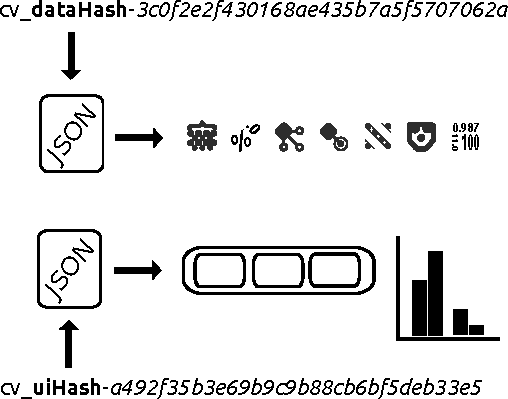
\includegraphics[width=8cm]{CubeViz/HashIllustration.pdf}
    \caption{Illustration zum Daten- und UI-Hash.}
    \label{fig:CubeViz_HashIllustration}
\end{figure}

\noindent
Die Abbildung \ref{fig:CubeViz_HashIllustration} veranschaulicht im unteren Teil neben einem anderen Hash mit Präfix auch den Visualisierungsselektor sowie die Visualisierung. Die Datei hinter diesem Hash enthält neben dem Namen der ausgewählten Visualisierung auch die dazu vorgenommenen Einstellungen. Da auch hier die Einstellungen in Form eines JSON-Objektes abgelegt sind, kann man dies leicht an den Client weiterreichen und im Browser weiterverarbeiten.

Der obige Mechanismus zur Speicherung getätigter Einstellungen arbeitet mit einer Konfigurationsdatei, welche festlegt, in welchem Rahmen die Visualisierung konfiguriert werden kann. Damit hat man als Betreiber von CubeViz die Möglichkeit, selbst zu entscheiden, was der Benutzer einstellen kann und was nicht. Die Konfigurationsdatei enthält selbst auch ein JSON-Objekt und bietet standardmäßig Einstellungen für maximal zwei Dimensionen. Der Aufbau der Datei basiert auf der Anzahl der mehrfachen Dimensionen. Beginnend bei Null wird pro Schritt eine Menge von Visualisierungstypen und ihren zugehörigen Einstellungen beschrieben.

Mehr als zwei Dimensionen, die jeweils mehr als ein Dimensionselement enthalten, werden von CubeViz bisher nicht unterstützt. Dies lag bisher an mangelhaften Visualisierungsbibliotheken, aber auch, weil der Mensch auf einer Fläche nur schwer einen mehrdimensionalen Körper begreifen kann.

CubeViz wählt die passende Visualisierung nach der Anzahl der mehrelementigen Dimensionen aus, im Folgenden als mehrfache oder multiple Dimensionen bezeichnet. Dies basiert auf der Auswahl im Modul des linken Hauptmenü und es wird die erste Visualisierung genutzt, die in der entsprechenden Liste der Konfigurationsdatei auftaucht. Dabei kann die Visualisierung einer Ebene in der Regel auch Beobachtungspunkte mit mehrfachen Dimensionen anzeigen, deren deren Anzahl kleiner als die aktuelle Ebene ist. Die Konfiguration für eine Visualisierung ist derzeit auf die HighCharts-Bibliothek auslegt. Ist die Einführung einer weiteren Bibliothek vorgesehen, dann werden ggf. interne Anpassungen nötig. 


%
% SSS
%
\subsection{Ist CubeViz ein Linked Data Mashup?}
\label{sec:chapterCubeVizAsLinkedDataMashup}

Bisher ist noch nicht ganz klar, ob CubeViz als Linked Data Mashup angesehen werden kann. Dieser Fragestellung soll nun schrittweise nachgegangen werden. 

Ist CubeViz überhaupt ein Mashup? Zunächst kann man davon ausgehen, dass CubeViz eine sich im Internet befindliche Software ist, die fremde Datenquellen abfragen kann, um basierend auf den aggregierten Daten Visualisierungen bereitzustellen. Über diese Visualisierungen und zusätzliche Benutzeroberflächen kann der Benutzer die statistischen Daten und ihre Meta-Daten explorieren. Mashup's besitzen eine Reihe von besonders ausgeprägten SOA-Prinzipien, welche im Folgenden für CubeViz überprüft werden. 

Die \textit{lose Kopplung}, \textit{maximale Abkapselung}\com{Überprüfung \\ SOA-Prinzipien} und \textit{Dienst-Autonomie} ist gegeben, da CubeViz als eigenständige Komponente in der Software OntoWiki arbeitet. Über eine Benutzeroberfläche sowie Schnittstellen zu lokalen SPARQL-Endpunkten kommuniziert sie mit der Außenwelt. Dabei stellt sie selbst Schnittstellen bereit, worüber Interessenten eigene Daten-Abfragen absetzen können. Hinsichtlich einer guten Auffindbarkeit muss CubeViz passen, denn es stellt keinerlei Beschreibung von sich und seinen Merkmalen über eine Auszeichnungssprache bereit. Die erleichterte Wiederverwendung ist nur begrenzt gegeben, da es zum jetzigen Zeitpunkt noch keine öffentliche Dokumentation über CubeViz und seine interne Arbeitsweise gibt, es sei denn, man zählt einen sehr umfangreich kommentierten Quellcode mit dazu. Da aber der Benutzer primär über die Benutzeroberfläche mit dem Dienst kommuniziert und diese unter Benutzeraspekten gestaltet wurde, sollte dies die vorherigen Defizite etwas abschwächen. Das letzte SOA-Prinzip, die \textit{Art der Nutzung}, fordert eine niedrige Einstiegshürde für unerfahrene Benutzer. In der jetzigen Version ermöglicht CubeViz die Nutzung für Unerfahrene, weil es leicht zu bedienende Benutzeroberflächen für seine Benutzer bereitstellt. Abschließend sei noch erwähnt,\com{Mashup- \\ Kategorien} dass CubeViz ein hybrides \mbox{Mashup} ist, denn es erfüllt die Kriterien sowohl für das \textit{Konsumenten-Mashup}, als auch \textit{Daten-Mashup}. 


\newpage
\noindent
Es bietet einen Zugang zu statistischen RDF-Daten für die technikaffine Öffentlichkeit, welche u.a. über die Konfiguration der Visualisierungen oder die Datenselektion die Daten explorieren kann. Ein Daten-Mashup wird CubeViz aber erst, wenn das darunterliegende OntoWiki fremde Erweiterungen nutzt, da es von sich aus keine fremden SPARQL-Endpunkte abfragen kann. Dies kann beispielsweise mithilfe der \textit{sparqlservices}-Erweiterung\footnote{\url{https://github.com/AKSW/sparqlservices.ontowiki}} von Michael Martin ermöglicht werden. Die Frage, ob CubeViz ein Mashup ist, kann nun mit ja beantwortet werden. Ergänzend dazu muss die Linked Data\com{Linked Data} Unterstützung überprüft werden. Wie bereits erwähnt, wird CubeViz erst zu einem Daten-Mashup, wenn es die Hilfe einer fremden Erweiterung in Anspruch nimmt. Dazu muss man wissen, dass \mbox{CubeViz} eine Datenselektion basierend auf einer vorherigen Modell-Auswahl bereitstellt. Ob diese Modelle aus lokalen oder entfernten Datenquellen stammen, ist dabei unerheblich. OntoWiki bietet in der Version 0.9.10 von sich aus keine Implementierung, um fremde Datenquellen abzufragen und deren Modelle bereitzustellen. Um diese Funktionalität nicht doppelt zu implementieren, installiert man die sparqlservices-Erweiterung in einem OntoWiki mit CubeViz. Dadurch erhält CubeViz mittelbar die Möglichkeit, Datensätze aus Modellen von entfernten Datenquellen zu nutzen. Es wurde gezeigt, dass CubeViz die Linked Data Technologie unterstützt. Der letzte Schritt ist nun die Überprüfung der Kriterien eines Linked Data Mashup's. \com{Linked Data Mashup} Diese forderten neben den bereits genannten Aspekten, dass es eine Ontologie gibt, welche die Domäne des Mashup's beschreibt. Diese Ontologie ist das DataCube-Vokabular, an dem CubeViz ausgerichtet ist. Linked Data Quellen werden nur unterstützt, wenn das genutzte OntoWiki mit entsprechenden Erweiterungen versehen wurde. Der Fakt mit den Anwendungsontologien, welche die genutzten Linked Data Quellen beschreiben, ist bereits gegeben, da nur Quellen aus der Domäne der statistischen Daten, die auf dem DataCube-Vokabular basieren, von CubeViz genutzt werden können.


%
% -----------------------------------------------------------------------------------------
%
\newpage
\section{Mashup-Erstellung aus verschiedenen Datensätzen}
\label{sec:sectionCreatingMashup}

In diesem Kapitel dreht sich alles um die Beschreibung eines Modells, welches als Grundlage für die Zusammenführung von DataCube-Datensätzen dient. Dazu bedarf es am Anfang einer Reihe von Vorarbeiten. Hierzu eine Liste:

\begin{itemize}
	\item \nameref{sec:chapterSameAs} (\ref{sec:chapterSameAs})
 	\item \nameref{sec:chapterInterpretationDC} (\ref{sec:chapterInterpretationDC})
 	\item \nameref{sec:chapterModelMergeDatasets} (\ref{sec:chapterModelMergeDatasets})
 	\item \nameref{sec:subsectionRequirementsAndSpecification} (\ref{sec:subsectionRequirementsAndSpecification})
\end{itemize}

\noindent
Zuerst wird erläutert, welche Definition den Begriffen Äquivalenz bzw. Gleichheit von Elementen zugrunde gelegt wird. Danach werden die bereits vorgestellten Bestandteile des DataCube-Vokabulars im Kontext dieser Arbeit interpretiert. Ist dies geschehen, wird auf das eigentliche Modell vorgestellt, was am Ende in einer Liste von Anforderungen mündet.

Um es vorwegzunehmen: Das Modell betrachtet in der Zusammenführung immer nur zwei Datensätze. Denn der Autor vertritt die These, dass man als Mensch nur zwei Dinge gleichzeitig effektiv vergleichen kann (\textit{F-90}).\com{Anforderung \\ F-90, S. \pageref{req:F90}}\label{req:F90source} Dazu werden in der Regel die Hände genutzt, um interessante Dinge erst anzufassen und sie dann zu untersuchen (wiegen, drehen,  ...). Genauer gesagt, man nimmt etwas in die eine Hand und etwas anderes in die andere. Danach schaut man sich beide Dinge abwechselnd an und vergleicht bestimmte Eigenschaften miteinander, wie das Gewicht oder die Farbe. Dieses Prinzip kann auf die Bestandteile des DataCube-Vokabulars übertragen werden. Wurde in dem genannten Beispiel ganz allgemein von Eigenschaften gesprochen, so wird sich das Modell nur auf gemeinsame Eigenschaften beschränken. Diese Eigenschaften können Eigenschaften eines Elementes oder ganz abstrakt sein, wie beispielsweise die Anzahl aller Beobachtungspunkte innerhalb eines Datensatzes. 

Diese These dient nicht nur als Grundlage für das Modell, sondern auch für den Aufbau der späteren Benutzerschnittstellen. Dies wird jedoch an entsprechender Stelle näher erläutert. Wie bereits gesagt, ist dies nur eine These und es soll nicht behauptet werden, Modelle mit einer abweichenden Konfigurationen wären von vornherein schlechter.

%
% SS
%
\subsection{Überprüfung auf Gleichheit}
\label{sec:chapterSameAs}

Die \textit{Gleichheit} von Ressourcen bezeichnet die komplette Übereinstimmung\com{Anforderung \\ F-20, S. \pageref{req:F20}} der jeweiligen URI's oder aber eine bestehende \textit{sameAs}-Beziehung zwischen ihnen (\textit{F-20}).\label{req:F20source} Gleichheit bedeutet dabei, dass jeweils zwei oder mehr untersuchte Elemente auf die gleiche Entität zeigen bzw. sie repräsentieren.

\noindent
Bei der Überprüfung auf Gleichheit gilt die bereits vorher erwähnte Annahme, dass eine Ressource über eine URI global eindeutig bezeichnet wird. Über einen Zeichenkettenvergleich innerhalb eines Programms kann geprüft werden, ob die URI's der Elemente übereinstimmen.

Eine andere Möglichkeit ist die Überprüfung hinsichtlich einer bestehenden \textit{sameAs}-Beziehung. Dazu wird davon ausgegangen, dass dem Programm bekannt ist, welches Modell bzw. welche Modelle die Datensätze enthalten. Es wird dann entweder auf eines der Modelle oder auf beide das folgende ASK-Query ausgeführt.\\

\begin{verbatim}
    @prefix owl: <http://www.w3.org/2002/07/owl#>
    ASK {
        <$dimensionUri1> owl:sameAs <$dimensionUri2> .
    }
\end{verbatim}

\noindent
Dabei müssen in dem ASK-Query die beiden Platzhalter, gekennzeichnet durch das Zeichen \verb|$|, jeweils durch die URI's der Dimensionen ersetzt werden. Das Query liefert nur eine binäre Antwort zurück, also ob es ein entsprechendes Tripel gefunden hat oder nicht.

Wie erwähnt, bezeichnen Ressourcen\com{Mehrdeutigkeit} entweder Informationsressourcen oder Nicht-Infor-mationsressourcen. Der Unterschied zwischen beiden liegt darin, dass letztere nicht klar definiert und damit elektronisch übertragen werden können. Als Beispiel sei eine Ressource genannt, die auf Leipzig zeigt. Sie kann damit einerseits eine Stadt Leipzig meinen, es gibt mehrere auf der Welt (eine in Deutschland und eine in Kanada\footnote{\url{https://en.wikipedia.org/wiki/Leipzig,_Saskatchewan}}), oder die Zeichenkette Leipzig oder die DBpedia-Seite\footnote{\url{http://dbpedia.org/page/Leipzig}} über Leipzig. Es ist daher wichtig, klar zu definieren, wann genau zwei Ressourcen das Gleiche \emph{meinen} und wann sie trotz gleicher Bezeichnung eine unterschiedliche Semantik besitzen. Aus diesem Grund macht es z.B. keinen Sinn, Ressourcen über deren Labels zu vergleichen, auch wenn dies in späteren Visualisierungen naheliegen kann.


%
% SS
%
\subsection{Weiterführende Auslegung der DataCube-Vokabular Elemente}
\label{sec:chapterInterpretationDC}

Die zu Beginn vorgestellten Bestandteile des DataCube-Vokabulars werden nun in den Rahmen dieser Arbeit eingebettet. Daraus soll ein Fundament entstehen, welches als Grundlage für das später zu entwickelnde Modell zur Zusammenführung von Datensätzen dient. Weiterhin sind manche Bestandteile nicht ausreichend in der Spezifikation definiert und es ist unklar, wo genau die Grenzen ihrer Anwendbarkeit liegen. Die hier stattfindende, streckenweise etwas philosophische Betrachtung dient ebenfalls dazu, die Bestandteile besser zu verstehen und einordnen zu können.

\noindent
Bei der Untersuchung wird oft mehr als nur eine mögliche Auslegung diskutiert. Es wird sich aber zeigen, dass eine Reihe von Betrachtungen und Untersuchungen nötig sind, um eine zufriedenstellende Einordnung in das Thema dieser Arbeit zu gewährleisten. Weiterhin kann es dazu kommen, dass bestimmte Auslegungen Einfluss auf andere haben. 


%
% SSS
%
\subsubsection{DataCube, Hyperwürfel, Beobachtung und Datensatz}

Die Begriffe \textit{DataCube}, \textit{Hyperwürfel} und \textit{Cube} werden im Rahmen dieser Arbeit als Synonym verwendet. Eine \emph{Beobachtung} ist ein (teilweise zeitlich begrenzter) Vorgang, bei dem einzelne Messungen durchgeführt werden. Die Messungen liegen dabei in Form von Beobachtungspunkten vor, welche jeweils Dimensionen und einen Messwert besitzen. Somit werden die Begriffe Beobachtung und \textit{Datensatz} als gleich erachtet. Ein Datensatz ist zudem eine echte Teilmenge eines DataCube.

%
% SSS
%
\subsubsection{Dimensionen und Dimensionselemente}

Dimensionen\com{Blickwinkel} können als einzelne Blickwinkel innerhalb einer Beobachtung angesehen werden -- als Analogie zu einem Gegenstand in einem Raum, den man sich ausgehend von verschiedenen Stellen in diesem Raum anschaut. Eine Dimension wäre damit extern anzusiedeln. Die Wahl der Blickwinkel wird von dem getroffen, der die Beobachtung durchführt bzw. die gemessenen Werte dokumentiert. Die ausgewählten Blickwinkel sind demnach das Produkt einer subjektiven Auswahl basierend auf bestimmten Kriterien, die zu dieser Auswahl geführt haben. Diese Kriterienauswahl an dieser Stelle soll nicht von Belang sein. 

Abbildung \ref{fig:DimensionelementAnalogy_PointOfViewParts} illustriert das soeben Beschriebene, wobei zwei verschiedene Interpretationen der Dimensionselemente dargestellt sind. Das Auge des Betrachters steht für den Betrachter an sich, der etwas beobachtet. Mit Beobachter muss dabei aber kein Mensch gemeint sein, sondern es kann sich genauso gut um eine Maschine handeln. \\

%
% Abbildung
%
\begin{figure}[h!]
    \centering
    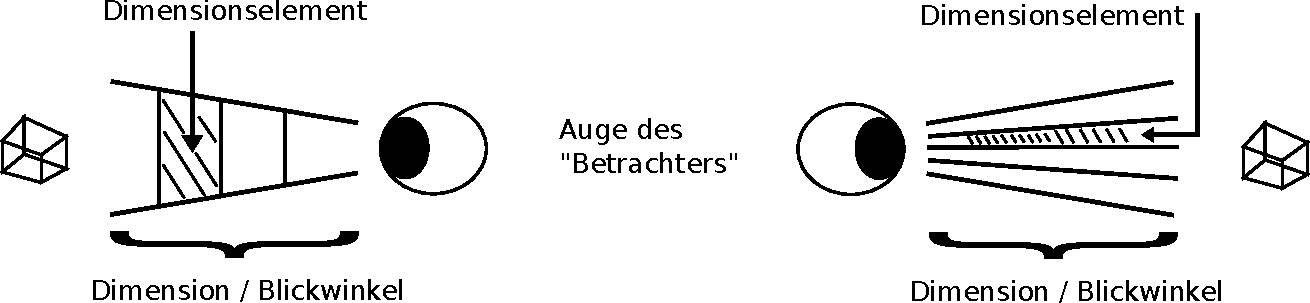
\includegraphics[width=12.5cm]{DataCube/DimensionelementAnalogy_PointOfViewParts.pdf}
    \caption{Illustration der Analogie über die Dimension als externer Blickwinkel.}
    \label{fig:DimensionelementAnalogy_PointOfViewParts}
\end{figure}

\noindent
Es stellt sich die Frage, welche Rolle die Dimensionselemente einnehmen. Bleibt man nämlich bei der obigen Analogie mit dem Blickwinkel, so müssten diese Teil des Blickwinkels sein. Zwei mögliche Auslegungen sind dazu auf obiger Abbildung \ref{fig:DimensionelementAnalogy_PointOfViewParts} dargestellt. Beide führen zu keiner zufriedenstellenden Erklärung.

\noindent
Eine andere Möglichkeit\com{Eigenschaft} wäre, dass man statt einer externen Betrachtung eine interne Betrachtung wählt. Dabei nimmt eine Dimension die Rolle einer Eigenschaft des zu beobachtenden Objektes bzw. Sachverhaltes ein. Die Eigenschaft darf dabei aber nur eine endliche Menge an Zuständen annehmen können. Auf der \mbox{Abbildung \ref{fig:DimensionelementAnalogy_ViewedObjectItself}} ist ein Beispiel illustriert, bei dem ein Gegenstand beobachtet wird und dabei drei Dimensionen (Eigenschaften) verwendet werden. 


\newpage
\noindent
Bei dieser Variante besitzt man sowohl eine klare Interpretation der Dimension als auch der Dimensionselemente. Weiterhin entspricht sie mehr der im DataCube-Vokabular vertretenen Ansicht, wie Dimensionen zu handhaben sind. Daher wird diese Ansicht im Folgenden vertreten. \\

%
% Abbildung
%
\begin{figure}[h!]
    \centering
    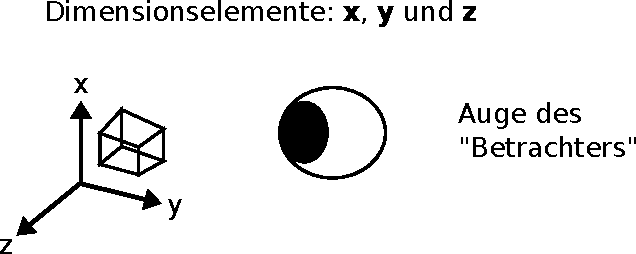
\includegraphics[width=6cm]{DataCube/DimensionelementAnalogy_ViewedObjectItself.pdf}
    \caption{Illustration der Analogie der Dimension als interne Eigenschaft des betrachteten Objektes.}
    \label{fig:DimensionelementAnalogy_ViewedObjectItself}
\end{figure}

\noindent
Theoretisch kann man während einer Beobachtung beliebig viele Blickwinkel benutzen. In dieser Arbeit wird dabei nur gefordert, dass jeder Blickwinkel eindeutig benennbar ist und deren Menge endlich und abzählbar ist.

Wie bereits erwähnt wurde, dienen die Dimensionen bzw. ihre Dimensionselemente dazu, die in einem Datensatz enthaltenen Beobachtungspunkte eindeutig zu identifizieren. Dabei nehmen die Dimensionen und Dimensionselemente eine ähnliche Rolle ein, wie die URI's in Linked Data bei der Ressourcenidentifikation. Setzt man den Term \emph{eindeutig} mit \emph{präzise} gleich, was wären wohl Antworten auf die folgende Problemstellung: 

\begin{quote}
    \emph{Man besitzt zwei Datensätze, wobei der eine zwei und der andere drei Dimensionen besitzt. Die zwei Dimensionen des ersten Datensatzes kommen auch in dem zweiten vor. Sind die Beobachtungspunkte des ersten Datensatzes dann noch eindeutig identifizierbar? Sind die Beobachtungspunkte des zweiten Datensatzes präziser identifizierbar als die des ersten Datensatzes?}
\end{quote}

\noindent
Ginge\com{Arten der \\Präzisierung} man davon aus, dass mit steigender Anzahl an Dimensionen auch der Grad der Genauigkeit der Beobachtungsdaten steigt, so hat man, salopp gesagt, in jedem Fall ungenaue Beobachtungsdaten, denn es könnte immer einen Datensatz geben, der alle Dimensionen des vorherigen Datensatzes besitzt und eine weitere. 
Diese Einsicht ist wohl nicht zielführend, aber daraus lassen sich für den späteren Vergleich zwischen Datensätzen einige Punkte ableiten. Teilen sich Datensätze gemeinsame Dimensionen, dann kann das darauf hindeuten, dass sie Beobachtungen repräsentieren, bei der die gleichen oder wenigstens ähnliche Aspekte beobachtet wurden. Je mehr Dimensionen vorhanden sind, desto präziser wird die Beobachtung beschrieben.

Eine andere Möglichkeit wäre, dass Dimensionen zwar für verschiedene beobachtete Aspekte stehen, aber deren Anzahl nichts über den Grad der Genauigkeit der Beachtung aussagt. Der Fokus liegt dann auf der Pluralität bzw. der Vielfalt innerhalb Beobachtung. Man kann dabei unterstellen, dass je mehr Dimensionen ein Datensatz besitzt, desto umfassender bzw. abwechslungsreicher die Betrachtung war.

Es lässt sich festhalten, dass man mit steigender Anzahl an Dimensionen die Beobachtung immer präziser oder abwechslungsreicher beschrieben wird. Dabei ist nicht ausgeschlossen, dass sich beide Möglichkeiten vermischen oder es gar noch weitere Möglichkeiten geben kann. Im Folgenden wird eine Mischung aus den beiden Ansätzen verwendet und damit auch obige Problemstellung beantwortet. Man besitzt zwar mit steigender Anzahl von Dimensionen eine präziser werdende Beschreibung eines Sachverhaltes, aber unter dem Gesichtspunkt, dass diese auch umfassender wird. Die Beobachtungspunkte des ersten Datensatzes sind eindeutig innerhalb ihres zugehörigen Datensatzes identifizierbar und die Beobachtungspunkte des zweiten Datensatzes bieten eine umfassendere Beobachtung als der erste.

Was bedeutet es, wenn sich zwei ungleiche Dimensionen, eine Menge von Dimensionselementen teilen? Diese Frage lässt eine Reihe von Antworten zu. Es könnte darauf hindeuten, dass es sich bei beiden Dimensionen um ähnliche Eigenschaften des Beobachteten handelt, womit Rückschlüsse auf das möglich wären, was beobachtet wurde. Hierbei könnte man unterstellen, dass mit steigender Anzahl gemeinsamer Dimensionselemente, der Grad der Ähnlichkeit der beiden Dimension steigt. Aber auch hier führt diese Betrachtung nicht weit, da es keinen nachvollziehbar definierten Schwellwert bei der Anzahl gemeinsamer Dimensionselemente gibt, ab dem die jeweiligen Dimensionen gleich sind.

Eine gemeinsame Nutzung von Dimensionselementen kann aber auch genau gar nichts bedeuten. Denn nur weil zwei Dimensionen gleich sind oder nicht, muss das nicht unbedingt in Wirklichkeit so sein bzw. vom Ersteller der Datensätze so gewollt gewesen sein. Hierbei spielt die Unterscheidung zwischen Informationsressourcen und Nicht-Informationsressourcen mit rein. Denn es wäre möglich, dass der Ersteller eine Nicht-Informationsressource für die Dimensionen genutzt hat. Dann kann man nämlich maschinell nicht mehr mit Gewissheit feststellen, ob die beiden bezeichneten Ressourcen gleich sind. Aber selbst wenn es sich um unterscheidbare URI's von Informationsressourcen handelt, kann es zu Problemen kommen, denn trotz ihrer Gleichheit können die damit bezeichneten Dimensionen zwei verschiedene Dinge meinen. Bei den Metadaten einer Beobachtung besteht auch keine Eindeutigkeit, wenn es um die Gleichheit von Elementen geht. Man kann sich hier nicht sicher sein, ob dies oder jenes wirklich gemeint war. 

In dieser Arbeit wird der letztere Fall angenommen: Es ist unklar, was es bedeutet, wenn sich zwei ungleiche Dimensionen gemeinsame Dimensionselemente teilen. Der Grund dafür ist der angesprochene Schwellwert, ab wieviel gemeinsamer Dimensionselemente zwei ungleiche Dimensionen gleich sind. Eine mögliche Festlegung des Schwellwertes wird als willkürlich angesehen. Daraus könnte folgen, dass die Maschine Gemeinsamkeiten \emph{erkennt} und darstellt, wo keine sind und den Benutzer womöglich zu falschen Annahmen führt. Das alles bedeutet aber nicht, dass zwei gleiche Dimensionen auf einmal ungleich sind. Eine gemeinsame URI oder sameAs-Beziehung stehen immer noch für die Gleichheit zweier Elemente, aber ein Rückschluss auf eine \emph{mögliche} Gleichheit aufgrund einer willkürlichen Grenze\com{Anforderung \\ F-30, S. \pageref{req:F30}} bei Ähnlichkeiten oder Gemeinsamkeiten soll untersagt sein (\textit{F-30})\label{req:F30source}.


\newpage
\noindent
Zu der gerade noch geführten Diskussion gehört noch folgende Frage: Wie geht man mit der Mehrdeutigkeit von Dimensionselementen um? Die Frage ist berechtigt, denn laut DataCube-Vokabular müssen Dimensionselemente keine Ressourcen, sondern können auch einfache Zeichenketten sein. Selbst wenn zwei Elemente mit dem gleichen Wort bzw. Wörtern bezeichnet werden, kann nicht ausgeschlossen werden, dass sie Verschiedenes meinen. Als Beispiel sei hier das Wort \emph{Leipzig} genannt: Es kann z.B. eine geographische Region sein, die Stadt Leipzig oder das Wort Leipzig. Im Rahmen dieser Arbeit werden die gleichen Kriterien bei der Überprüfung von Dimensionselementen auf Gleichheit angenommen, wie auch schon vorher bei den Dimensionen. Daraus folgt ebenfalls, dass Dimensionselemente ohne gültige URI von vornherein als ungleich angesehen werden.

%
% SSS
% 
\subsubsection{Der Messwert eines Beobachtungspunktes}
\label{sec:chapterInterpretationOfMeasure}

%
% Anforderung
%
Die im Rahmen einer Beobachtung gemessenen Ereignisse oder Zustände müssen\com{Anforderung \\ F-80, S. \pageref{req:F80}}\label{req:F80source} als reelle Zahl vorliegen. Ein Beispiel für eine nicht auf Zahlen basierte Lösung, wäre das Messen von Farbveränderungen innerhalb eines Zeitabschnittes. 

Der Messwert kann als eine Art besondere Dimension angesehen werden, also einen anderen Blickwinkel auf das beobachtete Objekt, bei dem die Elemente des Blickwinkels Zahlen sind. Genau wie bei Dimensionen, können auch Messwerte aus verschiedenen Datensätzen gleich oder unterschiedlich zueinander sein. Was würde es bedeuten, wenn zwei Messwerte aus jeweils verschiedenen Datensätzen gleich sind? Dafür gibt es eine Reihe von Interpretationen.

Eine Gleichheit kann zum einen auf den Fakt hinweisen, dass das Gleiche gemessen wurde. Weil aber Ressourcen mehrdeutig sein können, kann man sich nicht zu 100 Prozent sicher sein, dass die Ersteller der beiden Datensätze mit den festgelegten Messwerten wirklich genau das Gleiche meinten. Weiterhin wird man in der Regel nicht die Konfigurationen kennen, mit der die Messwerte ermittelt wurden. Dabei meint Konfiguration alles, womit man etwas messen kann, also insbesondere physisch vorhandene Apparaturen oder Messungen durch einfaches Abzählen vorhandener Elemente.


%
% Anforderung
%
\label{req:F230source}
\label{req:F240source}
\label{req:F340source} 
Selbst wenn Messwerte verschieden sind, muss das noch lange nicht bedeuten, dass im Endeffekt zwei völlig getrennte Dinge gemessen wurden. Die Schlussfolgerung, die der Arbeit nun zu Grunde liegt, ist, dass die Behandlung des Messwertes dynamisch erfolgen muss und der Benutzer\com{Anforderungen \\\\ \mbox{F-230, S. \pageref{req:F230}} \\\\ \mbox{F-340, S. \pageref{req:F340}} \\ \mbox{F-240, S. \pageref{req:F240}}} die Möglichkeit besitzt, dies selbst zu steuern. Dazu gehört, dass er die Möglichkeit besitzt, die gemessenen Werte einzeln anzupassen (\textit{F-230}) sowie sie in Form einer Normalisierung einander anzugleichen. Mit Normalisierung ist hier die Veränderung aller gemessenen Werte eines Datensatzes unter Nutzung einer Formel gemeint, bei der der Wert durch Einsetzen in die Formel verändert wird (\textit{F-340}). Dem Benutzer muss bei all dem möglich sein, die ursprünglichen Messwerte zu erkennen. (\textit{F-240})


%
% SSS
% 
\subsubsection{Der Beobachtungspunkt als Teil einer Beobachtung}

Ein Beobachtungspunkt ist ein einzelner gemessener Aspekt während einer Beobachtung. Eine Beobachtung ist somit diskret und besteht nur aus einzelnen Beobachtungspunkten. Jeder einzelne Beobachtungspunkt wird über die Dimension respektive deren einzelne Dimensionselemente eindeutig innerhalb eines Datensatzes identifiziert. Im Folgenden werden ein paar kontroverse Fälle diskutiert, die im Zusammenhang mit den Beobachtungspunkten eintreten können. Dabei geht es nicht vordergründig darum, eine Lösung zu finden, sondern darum, gewisse Problematiken zu umreißen und einen möglichen Umgang mit ihnen aufzuzeigen.

Basierend auf dem DataCube-Vokabular sind Beobachtungspunkte direkt mit der Beobachtung verbunden, bei der sie getätigt wurden. Es ist aber theoretisch möglich, dass es einen weiteren Datensatz gibt, der einen Beobachtungspunkt mit der gleichen URI enthält. Was bedeutet das? Eine naheliegende Erklärung wäre, dass hier zwei \mbox{Beobachtungen} stattgefunden haben, welche beide den gleichen Aspekt innerhalb ihrer Messungen haben. Haben beide Datensätze jeweils die gleichen Dimensionen und Dimensionselemente für den gemeinsamen Beobachtungspunkt verwendet, so muss man sich den gemessenen Wert anschauen. Ist dieser ebenfalls gleich, wurde wohl im zweiten Datensatz zumindest eine ähnliche Beobachtung mit teilweise übereinstimmenden Daten durchgeführt. Unterscheiden sich hingegen die gemessenen Werte, könnte das darauf hindeuten, dass hier die gleiche Messung nochmals oder mit einer veränderten Konfiguration durchgeführt wurde.

Sind bei gleichen Beobachtungspunkten auch die Dimensionen bzw. Dimensionselemente verschieden, dann kann postuliert werden, dass hierbei der gleiche Fakt unter verschiedenen Sichtweisen gemessen wurde. Es zeigt sich, dass es ein Wechselspiel zwischen den einzelnen Beobachtungspunkten und den jeweiligen Beobachtungen geben kann. Daher soll es in der zu entwickelnden Software dem Benutzer in irgendeiner Form möglich sein, die Beobachtungspunkte auf verschiedene Arten zu untersuchen.


%
% SS
%
\subsection{Modell zur Zusammenführung zweier Datensätze} 
\label{sec:chapterModelMergeDatasets}

In diesem Kapitel und seinen Unterkapiteln wird ein Modell erarbeitet, um zwei verschiedene Datensätze und ihre Beobachtungspunkte so zusammenzuführen, dass man sie vergleichen kann. Am Ende sollen die zusammengeführten Datensätze in einem neuen, künstlichen Datensatz aufgehen, welcher dann durch die Nutzung von CubeViz visualisiert und exploriert werden kann. Der Schwerpunkt bei der Zusammenführung liegt in der Erstellung valider JSON-Objekte, welche die jeweiligen DataCube-Elemente repräsentieren. Während dieses Kapitels werden weitere Anforderungen formuliert, welche später die Grundlage der zu entwickelnden Software werden. Es folgt eine Übersicht der Unterkapitel:

\begin{itemize}

    \item \nameref{sec:chapterModelRDFLvl} (\ref{sec:chapterModelRDFLvl})
    
    \item \nameref{sec:chapterModelToolLvl} (\ref{sec:chapterModelToolLvl})
    
    \item \nameref{sec:chapterModelNamespace} (\ref{sec:chapterModelNamespace})    
    
    \item In darauffolgenden Unterkapiteln wird jeweils die Zusammenführung einer Gruppe von DataCube-Elementen erläutert. Von jedem Element wird neben den Eigenschaften auch deren jeweilige Rolle in dem am Ende entstehenden zusammengeführter Datensatz beschrieben.
    
    \item \nameref{sec:subsectionRequirementsAndSpecification} (\ref{sec:subsectionRequirementsAndSpecification})
    
\end{itemize}

\noindent
Der Grund für die Entwicklung eines solchen Modells war, dass CubeViz als RDF-Browser für DataCube-Daten konzipiert wurde und daher nur mit Datensätzen umgehen kann. Aus diesem Grund müssen die beiden zu vergleichenden Datensätze unter gewissen Gesichtspunkten in einen neuen Datensatz überführt werden. Diese Gesichtspunkte werden nachfolgend näher vorgestellt. Neben der Möglichkeit der Exploration und Visualisierung liegt ein weiterer Grund darin, dass durch die Bereitstellung dieses Modells für eine spätere Verwendung auch andere Interessierte die Daten explorieren können. Der erstellte DataCube soll im Folgenden als \textit{zusammengeführter DataCube} bezeichnet. 

Ein übergeordnetes Ziel bei der Zusammenführung ist, dass die ursprünglichen Daten ersichtlich und zugänglich bleiben. \com{Vgl.\\ Anforderung\\ F-10, S. \pageref{req:F10source}}Deshalb sollen über entsprechende Relationen die jeweiligen Informationen, wie beispielsweise die URI eines Elementes, angebunden werden. Auf diese Weise soll es später dem Betrachter ermöglicht werden, nachzuvollziehen, was worauf basiert. Dies entspricht dem Mashup-\nameref{sec:MashupPrinciple-Original}.

Während der Erstellung eines zusammengeführten Datensatzes werden semantisch zusammengehörige Gruppen konstruiert, deren Bestandteile wiederum künstliche Elemente sind, welche in der Regel aus jeweils einem Element der beiden Datensätze konstruiert wurden. Diese Konstruktion wird unterteilt in zwei getrennte Ebenen, die Tool-Ebene und die RDF-Ebene.  

Der Begriff \emph{künstlich}\com{künstlich} wurde hier gewählt, weil die damit bezeichneten Elemente nur Hilfsstrukturen sind. Sie besitzen nicht wirklich eine eigene Semantik, sondern dienen lediglich als Proxy zwischen dem Pendant oder den beiden Pendants, aus denen sie hervorgegangen sind. \com{Anforderung \\ F-50, S. \pageref{req:F50}}Daher besitzen sie im Wesentlichen nur die nötigsten DataCube-Relationen, um valide DataCube-Elemente zu sein (\textit{F-50})\label{req:F50source}, eine aussagekräftige Bezeichnung (Titel und Kommentar) für die Benutzeroberfläche sowie Relationen zu den beiden Pendants. Im Folgenden werden die beiden Ebenen einzeln vorgestellt.


%
% SSS
% 
\subsubsection{Die RDF-Ebene}
\label{sec:chapterModelRDFLvl}

Auf der RDF-Ebene werden alle nötigen Relationen gesetzt, damit am Ende\com{Vgl. \\ F-10, S. \pageref{req:F10source}} ein valides DataCube-Element entsteht. Weiterhin werden Relationen (\textit{dct:source} bzw. \textit{owl:sameAs}) zu den jeweiligen Pendants gesetzt, aus denen das Element hervorgegangen ist. Diese Pendants sollen damit später für den Benutzer zugänglich\com{Anforderung \\ F-40, S. \pageref{req:F40}} \label{req:F40source} sein. Ergänzend dazu sei erwähnt, dass die RDF-Informationen dem Betrachter bei Bedarf präsentiert werden müssen (\textit{F-40}).


%
% SSS
%
\subsubsection{Die Tool-Ebene}
\label{sec:chapterModelToolLvl}

Die Tool-Ebene wird stark von dem genutzten Programm CubeViz beeinflusst. Bei diesem liegt der Großteil der Programmlogik in der Benutzerschnittstelle und damit in Form von JavaScript und JSON vor. Die zu visualisierenden Daten werden in Form von JSON-Objekten organisiert, daher setzt man bei der Zusammenführung der Datensätze auch hier an. Jedes DataCube-Element wird durch ein eigenständiges JSON-Objekt repräsentiert, welches ausschließlich aus Schlüssel-Wert-Paaren besteht. Diese Paare lassen sich in zwei Gruppen einteilen. 

In ersterer Gruppe sind die Schlüssel die Relationen, die das jeweilig zu erzeugende DataCube-Element besitzen muss. Die zugehörigen Schlüssel-Werte sind die gleichen, wie auf der RDF-Ebene.

Bei der zweiten Gruppe sind die Schlüssel CubeViz-spezifische Zeichenketten mit dem Präfix \verb|__cv_|. Deren Aufgaben bestehen darin, das Verhalten von CubeViz mit dem Umgang der jeweiligen Elementen zu steuern. Zum Beispiel behandelt CubeViz den Wert des Schlüssels \verb|__cv_niceLabel| als vollwertigen Titel eines Elementes und stellt ihn in der Benutzeroberfläche dar. 


%
% SSS
%
\subsubsection{Eigener Namensraum für künstliche Elemente}
\label{sec:chapterModelNamespace}

Nachfolgend sollen alle Elemente, die zu einem zusammengeführten Datensatz gehören, den gleichen Namensraum in der URI nutzen. Dafür wird die URI von CubeViz als Ausgangspunkt genutzt. Es folgt die Darstellung des Schemas:

\begin{quote}
	Namensraum: \verb|[DOMAIN]/cubeviz/export/datacube/[HASH]#|
\end{quote}

Diese URI-Struktur nutzt die aktuelle Domain sowie den Controller \emph{cubeviz} und die Action \emph{export}. Danach folgt der \emph{Hash} und eine \emph{Raute}, an der später die jeweiligen Elementnamen angefügt werden. Die Generierung des Hashs soll basierend auf den ermittelten Daten der ausgewählten Datensätze stattfinden, damit Hash und Daten eineindeutig sind.

%
% SSS
%
\subsubsection{Erstellung eines künstlichen Datensatzes}

%
% Abbildung
%
\begin{figure}[h!]
    \centering
    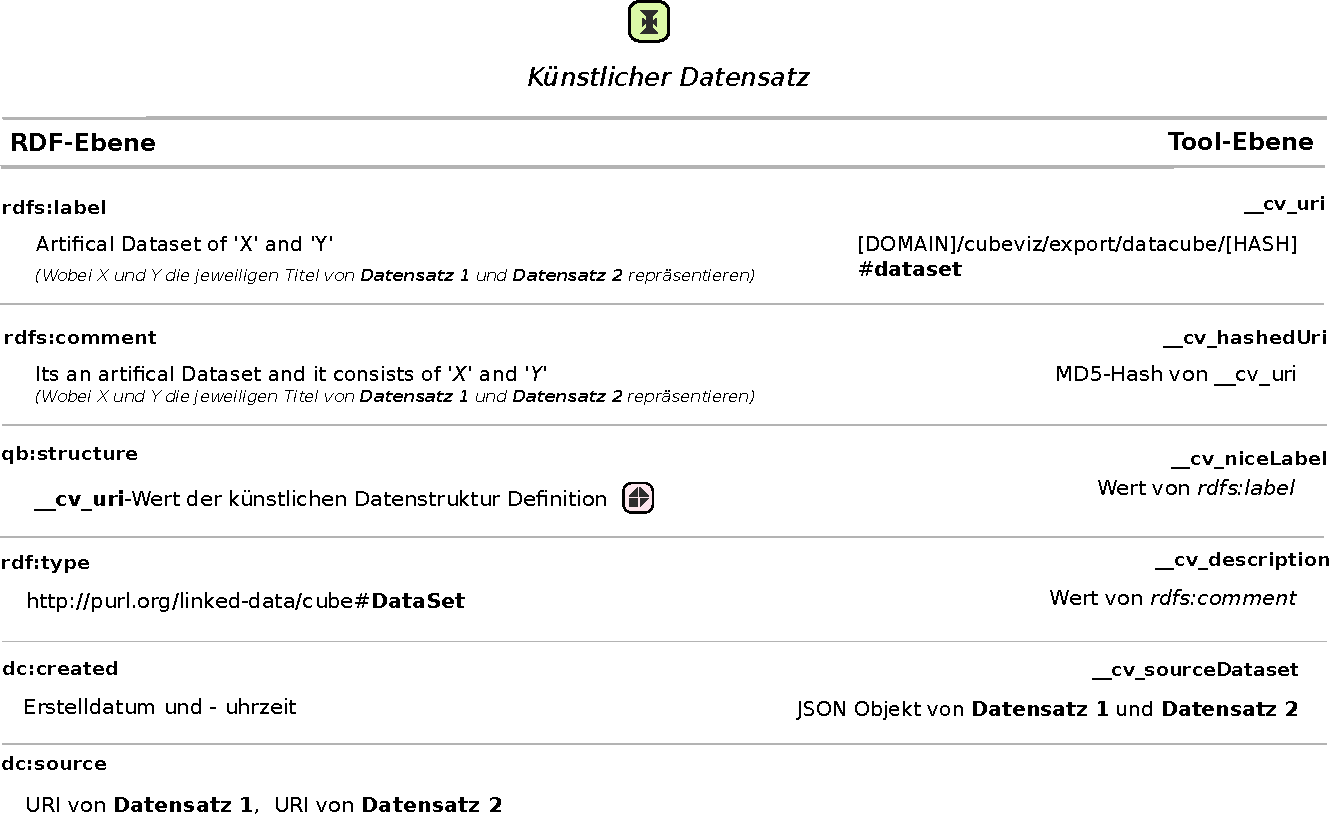
\includegraphics[width=15cm]{MergedDataCube/Dataset.pdf}
    \caption{Illustration der Bestandteile eines künstlichen Datensatzes.}
    \label{fig:MergedDataCube_Dataset}
\end{figure}

\noindent
Ausgangspunkt bei der Erstellung eines künstlichen Datensatzes und all seiner Bestandteile sind zwei andere valide Datensätze. \com{Anforderung \\ F-60, S. \pageref{req:F60}}Es wird gefordert, dass sich die Datensätze mindestens eine gemeinsame Dimension teilen (\textit{F-60})\label{req:F60source}. Ist dem nicht so, dann wird angenommen, dass sie nicht vergleichbar sind und können demnach auch nicht zusammengeführt werden. Der Grund für die Forderung mindestens einer gemeinsamen Dimension ist, dass man eine gemeinsame Grundlage für die jeweiligen Beobachtungspunkte besitzt. 

\newpage
\noindent
Für den Betrachter mag es bei der Betrachtung ersichtlich sein, ob zwei Datensätze zusammengeführt werden können oder nicht, aber die Maschine kann diese kognitive Leistung nicht durchführen. Weiterhin soll der zusammengeführte Datensatz am Ende ebenfalls ein gültiger Datensatz im Sinne des DataCube-Vokabulars sein, was ebenfalls bedeutet, dass alle seine Beobachtungspunkte\com{Anforderung \\ F-360, S. \pageref{req:F360}} die gleichen Dimensionen und Messwerte besitzen müssen (\textit{F-360})\label{req:F360source}. Daher ist es nicht möglich, einfach zwei beliebige Datensätze zu mischen.

Der zusammengeführte Datensatz dient später als eine Art Container für die restlichen DataCube-Elemente. Die Bestandteile dieses Datensatzes sind auf Abbildung \ref{fig:MergedDataCube_Dataset} illustriert. Diese sind getrennt nach den beiden Ebenen, links die RDF-Ebene und rechts die Tool-Ebene, jeweils mit den zugehörigen Eigenschaften. Der Datensatz besitzt im Wesentlichen einen Titel, eine knappe Beschreibung, das Erstellungsdatum mit Uhrzeit, einen Typ und Relationen auf die beiden genutzten Datensätze.

Bei den Relationen werden die URI's der beiden Datensätze sowie deren JSON-Objekte angebunden. Wie zuvor erwähnt, wurde in CubeViz der Großteil der Logik im Frontend in JavaScript realisiert, welches auch die abgefragten DataCube-Informationen in Form von eigenständigen Objekten verwaltet. Unter der Eigenschaft \verb|__cv_sourceDimension| sollen die beiden Objekte der Datensätze hinterlegt werden.

%
% SSS
%
\subsubsection{Erstellung einer künstlichen Komponenten-Spezifikation für eine Dimension}
\label{sec:chapter_mergeDimensions}

Es folgt eine mengentheoretische Betrachtung der verschiedenen Fälle, die bei der Zusammenführung von Dimensionen eintreten können. Wir unterscheiden dabei zwischen einem Paar gleicher Dimensionen und mehr als einem Paar. Die Betrachtungen beanspruchen keine Vollständigkeit. Es soll angenommen werden, man hat ein Paar gleicher Dimensionen, die aus zwei verschiedenen Datensätzen stammen. Dabei können vier Fälle beim Zusammenführen dieses Paares auftreten, welche auf Abbildung \ref{fig:4BasicCases_1DimEqual} dargestellt sind. Jeder dieser Fälle beschreibt, ob und in welcher Form sich die Dimensionen jeweils Dimensionselemente teilen. Folgendes sei gegeben:

\begin{itemize}
    \item $D1'$ und $D1''$ sind zwei gleiche Dimensionen
    \item $DE'$ entspricht der Menge der Dimensionselemente von $D1'$
    \item $DE''$ entspricht der Menge der Dimensionselemente von $D1''$
    \item Gleiche Dimensionen sind auf den Abbildungen als Kreise, ungleiche Dimensionen als Vierecke dargestellt\\
\end{itemize}

\begin{figure}[!htb]
\minipage{0.30\textwidth}
    \centering
    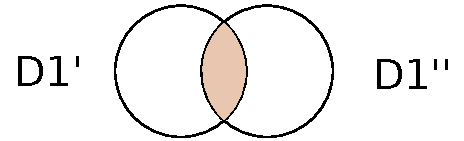
\includegraphics[width=3cm]{CaseDifferentiation/GeneralCase_2EqualDim_ShareSomeDe.pdf}
    \label{}
\endminipage\hfill
\minipage{0.20\textwidth}%
    \centering
    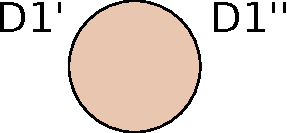
\includegraphics[width=1.9cm]{CaseDifferentiation/CaseDifferentiation_1SameDim_AllDePairPartnered.pdf}
    \label{}
\endminipage
\minipage{0.25\textwidth}%
    \centering
    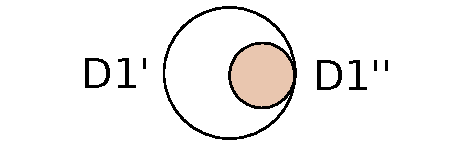
\includegraphics[width=3cm]{CaseDifferentiation/GeneralCase_2EqualDim_DimInDim.pdf}
    \label{}
\endminipage
\minipage{0.25\textwidth}
    \centering
    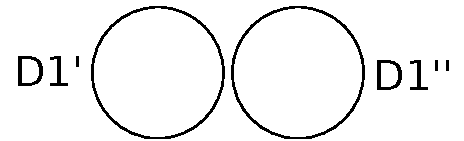
\includegraphics[width=3cm]{CaseDifferentiation/GeneralCase_2EqualDim.pdf}
    \label{}
\endminipage\hfill
\caption{Mengentheoretische Betrachtung der vier Fälle bei einem Paar gleicher Dimensionen.}
\label{fig:4BasicCases_1DimEqual}
\end{figure}

\noindent
Die Fälle auf Abbildung \ref{fig:4BasicCases_1DimEqual} werden nun von links nach rechts einzeln erläutert und jeweils mit einer Formel versehen.

%
% P
%
\paragraph{Fall 1} Es teilen sich zwei Dimensionen mindestens ein Dimensionselement. Da es sich hier um die gleichen Dimensionen handelt, werden später deren Dimensionselemente in eine Menge zusammengeführt. 

$$
    \exists de' \in D1', \exists de'' \in D1'': de' = de''
$$


%
% P
%
\paragraph{Fall 2} Hierbei teilen sich zwei Dimensionen jeweils alle Dimensionselemente, ausgedrückt über folgende Formel:

$$
    \forall de' \in D1', \forall de'' \in D1'': de' = de''
$$


%
% P
%
\paragraph{Fall 3} Bei diesem Fall sind alle Dimensionselemente der einen Dimension auch Teil der anderen, wobei die andere mindestens ein eigenes Dimensionselement besitzt.

$$
    \exists de' \in D1', \exists de'' \in D1'': de' \in D1'' \wedge de'' \not\in D1'
$$


%
% P
%
\paragraph{Fall 4} Im letzten Fall der Abbildung teilen sich die Dimensionen keine Dimensionselemente. Dazu die Formel:

$$
    \forall de' \in D1', \forall de'' \in D1'': de' \neq de''
$$

\noindent
\\Es ist möglich, dass die beiden Datensätze noch weitere Dimensionen enthalten, die es im jeweils anderen nicht gibt. Falls sich diese Dimensionen mindestens ein Dimensionelement teilen, können folgende Fälle auftreten: \\

\begin{figure}[!htb]
\minipage{0.25\textwidth}%
\centering
  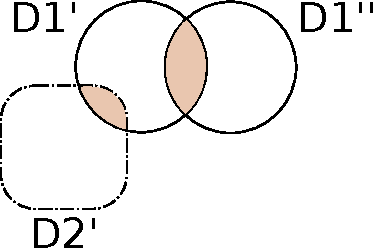
\includegraphics[width=2.5cm]{CaseDifferentiation/CaseDifferentiation_1SameDim_SomeDePairPartnered_ConnUnequalDimDiffDS.pdf}
  \label{}
\endminipage
\minipage{0.25\textwidth}%
\centering
  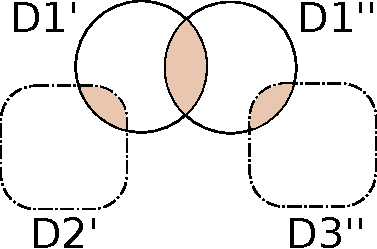
\includegraphics[width=2.5cm]{CaseDifferentiation/CaseDifferentiation_1SameDim_SomeDePairPartnered_ConnEqualUnequalDim.pdf}
  \label{}
\endminipage
\minipage{0.25\textwidth}%
\centering
  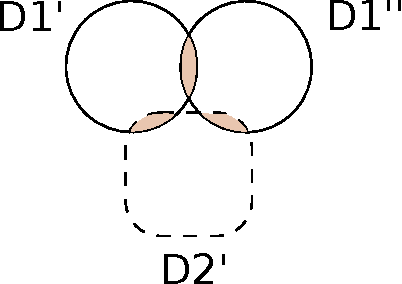
\includegraphics[width=2.5cm]{CaseDifferentiation/CaseDifferentiation_1SameDim_SomeDePairPartnered_UnequalDimConnectBoth.pdf}
  \label{}
\endminipage
\minipage{0.25\textwidth}%
\centering
  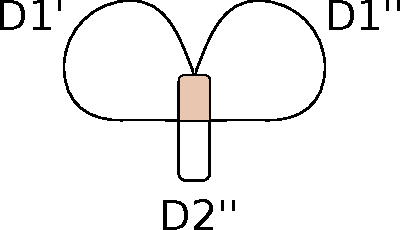
\includegraphics[width=2.5cm]{CaseDifferentiation/CaseDifferentiation_1SameDimAnd1Diff_AllDimSameDE.pdf}
  \label{}
\endminipage
\caption{Vier Fälle mit gleichen und ungleichen Dimensionen bei einem Paar gleicher Dimensionen.}
\label{fig:4BasicCases_1DimEqual_4ExtCases}
\end{figure}

\noindent
Diese Fälle werden nicht einzeln erläutert, da sie ausreichend sind, um zwei Muster zu illustrieren. Diese Muster sind die \textit{Verkettung} und der \textit{Zyklus}:

\begin{itemize}
    \item Bei einer \emph{Verkettung}\com{Verkettung} teilen sich paarweise mindestens zwei Dimensionen jeweils mindestens ein Dimensionselement. (Abb. \ref{fig:4BasicCases_1DimEqual_4ExtCases}: Bild 1 und 2)
    \item Ein \emph{Zyklus}\com{Zyklus} ist eine Verkettung, wobei die Start- und Enddimension jeweils gleich sind. (Abb. \ref{fig:4BasicCases_1DimEqual_4ExtCases}: Bild 3)
\end{itemize}


\noindent
Die ersten beiden Illustrationen der Abbildung \ref{fig:4BasicCases_1DimEqual_4ExtCases} sind Verkettungen, die dritte ein Zyklus. Die letzte Abbildung ganz rechts stellt einen Sonderfall dar, weil sich bei diesem alle drei Dimensionen die gleichen Dimensionselemente teilen. Treten diese Muster auf, so können sie auf eine Gemeinsamkeit zwischen den verketteten Dimensionen hindeuten. In der paarweisen Zusammenführung von zwei Dimensionen hingegen sollen nur gleiche Dimensionen zusammengeführt werden. Ungleiche Dimensionen, die sich Dimensionselemente teilen, sollen trotzdem weiterhin als ungleich gelten. \\

\begin{figure}[!htb]
\minipage{0.33\textwidth}
    \centering
    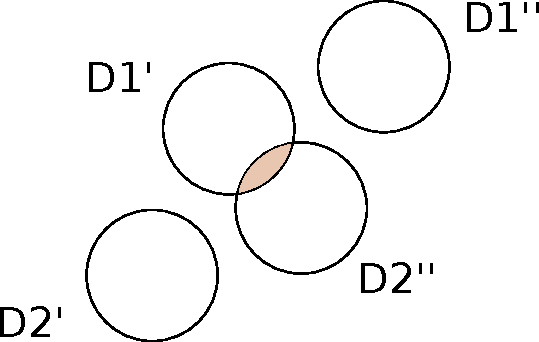
\includegraphics[width=2.7cm]{CaseDifferentiation/CaseDifferentiation_2SameDim_Cross_1DimSomeDePairPartnered_1DimNoDePairPartnered.pdf}
  \label{}
\endminipage\hfill
\minipage{0.33\textwidth}
    \centering
    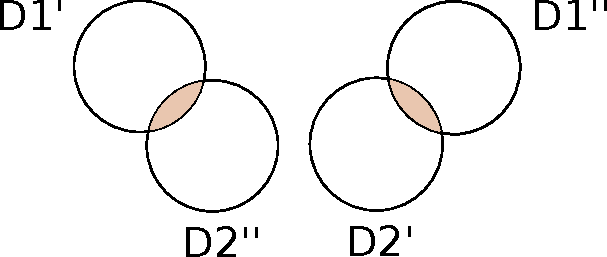
\includegraphics[width=2.9cm]{CaseDifferentiation/CaseDifferentiation_2SameDim_Cross_1DimSomeDePairPartnered_Cross_1DimSomeDePairPartnered.pdf}
  \label{}
\endminipage\hfill
\minipage{0.33\textwidth}%
    \centering
    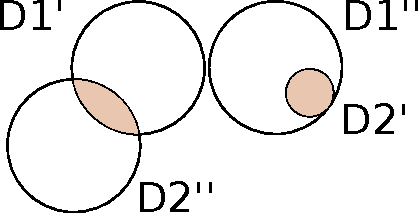
\includegraphics[width=2.3cm]{CaseDifferentiation/CaseDifferentiation_2SameDim_TwoDimSeperate_OneDiffInAnother_TwoDiffShareSomeDE.pdf}
  \label{}
\endminipage
\end{figure}

\begin{figure}[!htb]
\minipage{0.33\textwidth}%
    \centering
    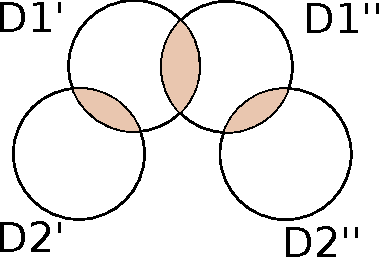
\includegraphics[width=2cm]{CaseDifferentiation/CaseDifferentiation_2SameDim_4DimSomeDePairPartnered_4Chaining.pdf}
  \label{}
\endminipage
\minipage{0.33\textwidth}%
    \centering
    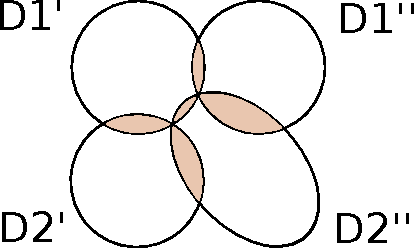
\includegraphics[width=2.3cm]{CaseDifferentiation/CaseDifferentiation_2SameDim_Cross_1DimSomeDePairPartnered_Circle.pdf}
  \label{}
\endminipage\hfill
\minipage{0.33\textwidth}%
    \centering
    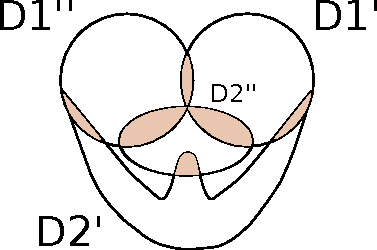
\includegraphics[width=2.1cm]{CaseDifferentiation/CaseDifferentiation_2SameDim_Cross_1DimSomeDePairPartnered_Cross_1DimSomeDePairPartnered_2DiffDSDimShareSameDe_2SameDSShareSameDe.pdf}
  \label{}
\endminipage
\caption{Acht ausgewählte Fälle bei mindestens zwei Paar gleicher Dimensionen.}
\label{fig:SelectCases_MoreAs1DimEqual}
\end{figure}

\noindent
Man nehme nachfolgend an, dass man mindestens zwei Paare mit gleichen Dimensionen vorliegen hat. Dabei können die gleichen Fälle auftreten wie bereits oben erläutert. Daneben können eine Reihe weiterer Fälle auftreten, acht davon sind auf der Abbildung \ref{fig:SelectCases_MoreAs1DimEqual} illustriert.

Bei all diesen Fällen treten ebenfalls wieder die bereits vorgestellten Muster der Verkettung und des Zyklus auf. Es stellt sich dabei die Frage, was es bedeutet, wenn zwei Paare gleicher Dimensionen sich jeweils Dimensionselemente teilen. Man könnte daraus schlussfolgern, dass all diese Dimensionen prinzipiell verwandt sind. Bei der Zusammenführung gilt auch hier, dass jedes Paar gleicher Dimensionen einzeln zusammengeführt wird. Teilen sich die Paare jeweils untereinander noch Dimensionselemente, dann soll dies nicht dazu führen, dass all diese Paare gemeinsam zusammengeführt werden. Wie bereits vorher erwähnt, deuten gemeinsame Dimensionselemente zwar auf ähnliche Dimensionen hin, bewirken aber nicht, dass diese Dimensionen als gleich betrachtet werden. Damit soll die Fallunterscheidung abgeschlossen sein. Der Vollständigkeit halber wurde im Anhang im Kapitel \ref{sec:Attachement_DimCases} eine detaillierte Auflistung der einzelnen Fälle eingefügt.

\noindent
Nun folgt die technische Sichtweise auf die Zusammenführung von Dimensionen. Für jede Dimension, die sich die beiden ausgewählten Datensätze teilen, wird eine künstliche Komponenten-Spezifikation erstellt. Deren Aufbau ist ähnlich dem des künstlichen Datensatzes und ist auf Abbildung \ref{fig:MergedDataCube_ComponentSpecificationDimension} dargestellt. Es wird hier die Relation \verb|qb:dimension| zu einer nicht existierenden Dimension erstellt. Später ist nur noch diese Dimensions-URI nötig, die eigentliche Ressource muss nicht existieren. Bei der URI-Generierung wird eine fortlaufende Nummer verwendet, repräsentiert durch den Platzhalter \emph{i}. Dieser startet bei null und wird für jede gemeinsame Dimension um eins hochgezählt. Das Gleiche passiert bei der Generierung der URI für die künstliche Komponenten-Spezifikation, denn es wird der gleiche Wert für den Platzhalter \emph{i} genutzt, so dass das gleiche \emph{i} für dieselbe Komponenten-Spezifikation nebst ihrer zugehörigen Dimension steht. 

Zu jeder Komponenten-Spezifikation\com{
\includegraphics[width=0.4cm]{semicon/dimensionElement2.pdf}} einer Dimension gehören auch Dimensionselemente. Diese werden aus den beiden Komponenten-Spezifikationen genommen und in einer Menge zusammengeführt. Dabei kann man verschiedene Wege gehen. 

Entweder man nimmt alle Dimensionselemente, wobei alle eine andere URI haben müssen, oder man entscheidet sich für die Nutzung\com{Anforderung \\ F-350, S. \pageref{req:F350}} jeweils aller gleichen oder ungleichen Dimensionselemente (\textit{F-350}).\label{req:F350source} Hat man sich für eine dieser Möglichkeiten entschieden, geht es um die eigentliche Zusammenführung und Anpassung der Dimensionselemente. Es ist nicht ausreichend, sie zusammen in eine Liste aufzunehmen, sondern es müssen Anpassungen vorgenommen werden, da sich durch die Zuweisung an eine neue Komponenten-Spezifikation beispielsweise auch der Typ(\verb|rdf:type|) der Dimensionselemente ändert. Alle Anpassungen sind in folgender Liste zusammengefasst:

\begin{itemize}

    \item Eigene \verb|URI| ändert sich in \verb|[DOMAIN]/cubeviz/export/datacube/[HASH]|\\\verb|#dimension|\textbf{\emph{i}}\verb|DimensionElement|\textbf{\emph{j}}

    \item Neuer Wert für \verb|rdf:type| ist nun \verb|[DOMAIN]/cubeviz/export/datacube/[HASH]|\\\verb|#dimension|\textbf{\emph{i}}

    \item Füge \verb|owl:sameAs|-Relation zur URI des ursprünglichen JSON-Objektes des Dimensionselementes hinzu

    \item Füge \verb|dct:source|-Relation zur URI des ursprünglichen Dimensionselementes hinzu
\end{itemize}

\noindent
Jedes Element erfährt diese Anpassungen. Dabei entsprechen die Platzhalter \emph{i} den fortlaufenden Nummern der Komponenten-Spezifikationen der Dimensionen und das \textbf{\emph{j}} den fortlaufenden Nummern der Dimensionselemente der aktuellen künstlichen Kompo-nenten-Spezifikation.

%
% Abbildung
%
\begin{figure}[h!]
    \centering
    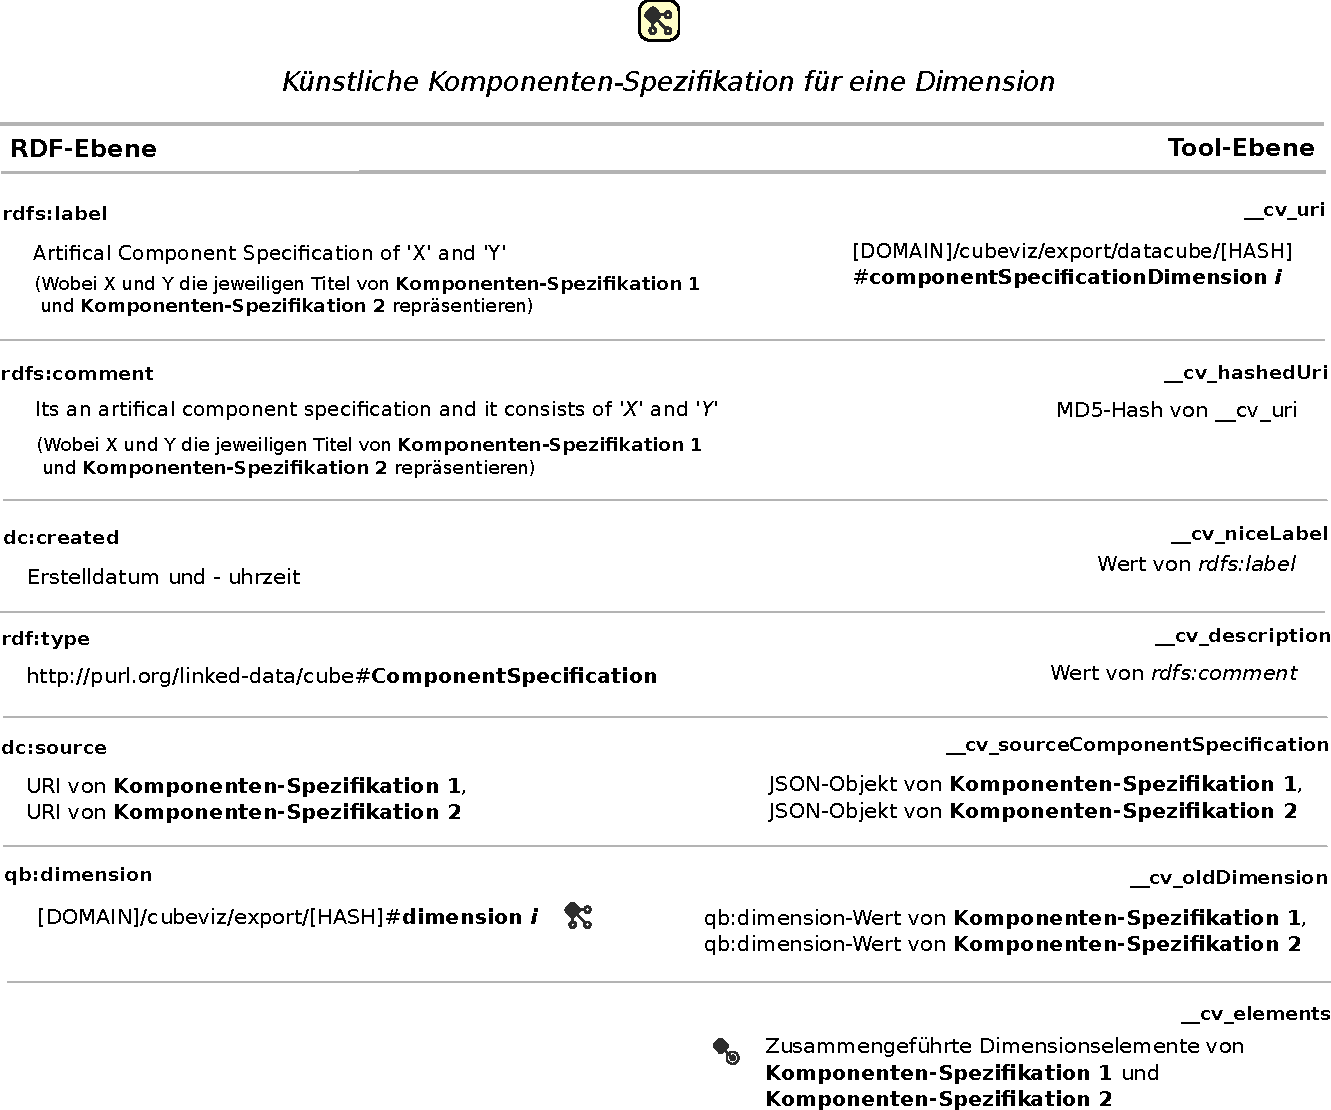
\includegraphics[width=15cm]{MergedDataCube/ComponentSpecificationDimension.pdf}
    \caption{Illustration der Bestandteile einer künstlichen Komponenten-Spezifikation für Dimensionen.}
    \label{fig:MergedDataCube_ComponentSpecificationDimension}
\end{figure}

%
% SSS
%
\subsubsection{Erstellung einer künstlichen Komponenten-Spezifikation für den Messwert}

Die Erstellung der Komponenten-Spezifikation für den Messwert gestaltet sich fast genauso, wie bei denen für die Dimensionen, nur dass es hier keine Dimensionselemente zu beachten gibt sowie keine fortlaufenden Platzhalter \textit{i} und \textit{j}. Es wird ebenfalls ein Titel und Beschreibungstext gesetzt sowie ein Erstellungsdatum, eine URI, ein Typ und Relationen zu den Pendants. Als Übersicht sei auf die Abbildung \ref{fig:MergedDataCube_ComponentSpecificationMeasure} verwiesen.

Im Folgenden wird festgelegt, dass die zusammenzuführenden Datensätze jeweils nur maximal einen Messwert besitzen. Es gibt Datensätze, bei denen das nicht zutrifft, daher wurde auf der Projekt-Seite von CubeViz ein Feature-Request dafür erstellt\footnote{\url{https://github.com/AKSW/cubeviz.ontowiki/issues/181}}. Dieser kann somit nach Abschluss der Arbeit noch implementiert werden.

Hinsichtlich der Semantik nimmt der Messwert im Vergleich zu den Dimensionen eine Sonderrolle ein. Es ist unerheblich, ob die jeweiligen Messwerte gleich sind oder nicht. Die dazugehörige Diskussion wurde im Unterkapitel \ref{sec:chapterInterpretationOfMeasure}\com{Kapitel \ref{sec:chapterInterpretationOfMeasure} \\ S. \pageref{sec:chapterInterpretationOfMeasure}} geführt.

Am Ende ist ausschlaggebend, dass es für den Betrachter nicht ersichtlich ist, welche Konfiguration von den Erstellern der statistischen Daten genutzt wurde, um die Messwerte zu ermitteln. Ohne allzu philosophisch zu werden, soll für das Modell angenommen werden, dass es niemals typgleiche Messwerte geben kann, egal ob die Komponenten-Spezifikationen die gleiche URI besitzen oder sich eine sameAs-Relation teilen.

%
% Abbildung
%
\begin{figure}[h!]
    \centering
    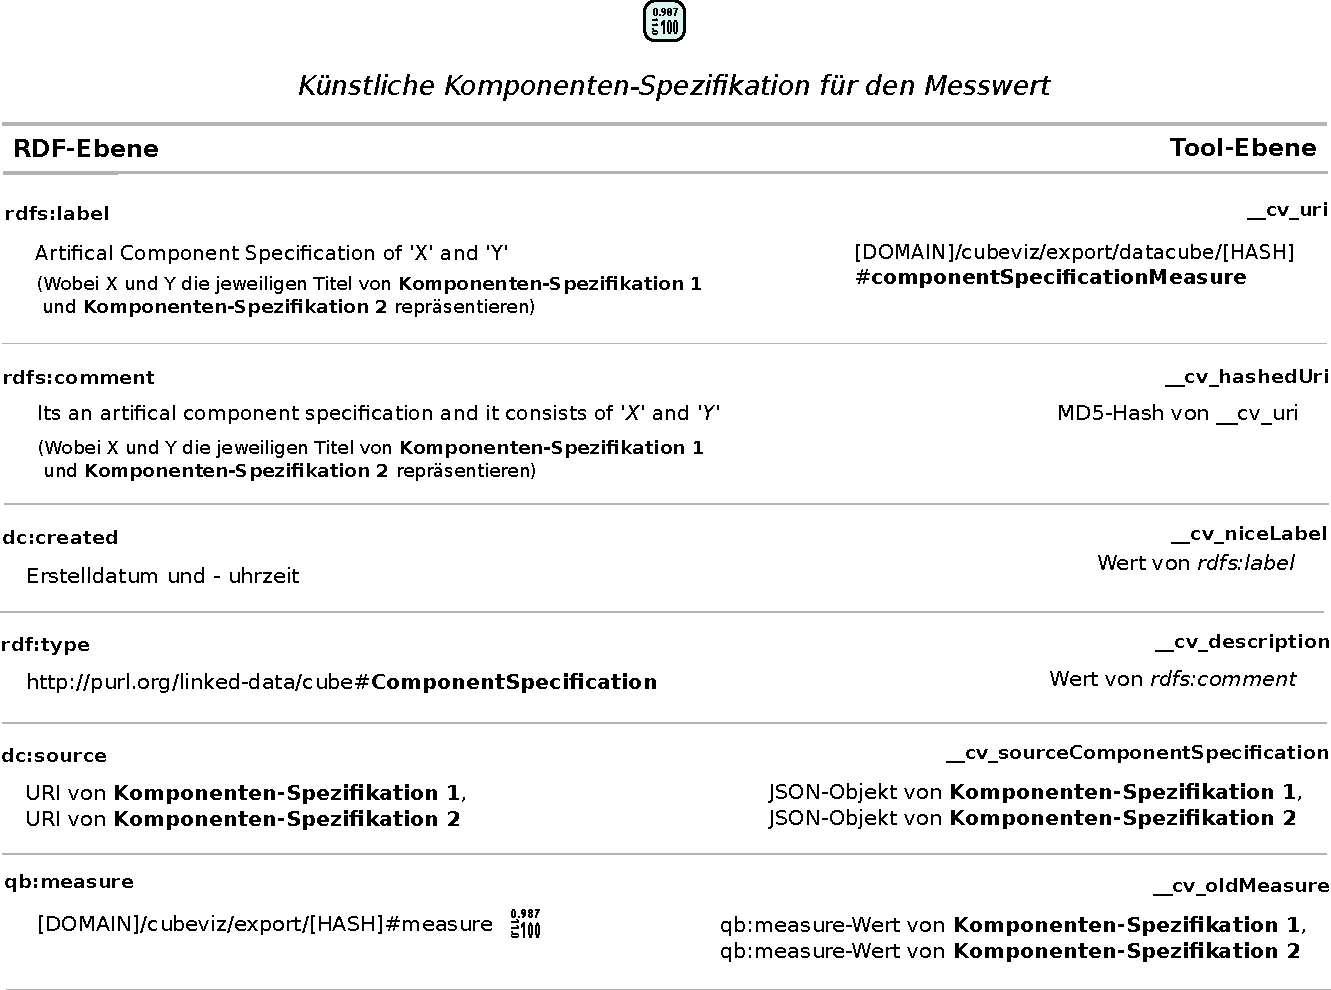
\includegraphics[width=15cm]{MergedDataCube/ComponentSpecificationMeasure.pdf}
    \caption{Illustration der Bestandteile einer künstlichen Komponenten-Spezifikation für den Messwert.}
    \label{fig:MergedDataCube_ComponentSpecificationMeasure}
\end{figure}

\noindent
Nichtsdestotrotz handelt es sich bei allen Messwerten um reelle Zahlen. Dies wurde bereits eingangs als Bedingung gesetzt. Zahlen können sich zwar auf riesige Skalen verteilen, aber sie besitzen alle die gleiche Semantik in dem Sinne, dass sie Zahlen sind. Aus diesem Grund wird bei der Erstellung der künstlichen Komponenten-Spezifikation eines Messwertes festgelegt, dass die späteren Beobachtungspunkte alle den gleichen Messwert bekommen. 

\newpage
\noindent
Um die Beobachtungspunkte aus den beiden Datensätzen gemeinsam anzuzeigen, ist es nötig, dass alle den gleichen Messwert zugewiesen bekommen. Der Grund dafür ist, dass CubeViz nur die Auswahl eines Messwertes zur selben Zeit erlaubt.


%
% SSS
%
\subsubsection{Erstellung einer künstlichen Datenstruktur Definition}

Die künstliche Datenstruktur Definition hat nichts gemein mit den jeweiligen Datenstruktur Definitionen der ausgewählten Datensätze. Sie dient lediglich dazu, den künstlichen Datensatz mit den jeweiligen künstlichen Komponenten-Spezifikationen der Dimensionen und des Messwertes zu verbinden. Aus diesem Grund besitzt sie keine Relationen zu anderen Pendants. Auf der folgenden Abbildung \ref{fig:MergedDataCube_DataStructureDefinition} findet man eine knappe Übersicht über die Bestandteile der künstlichen Datenstruktur Definition. \\

%
% Abbildung
%
\begin{figure}[h!]
    \centering
    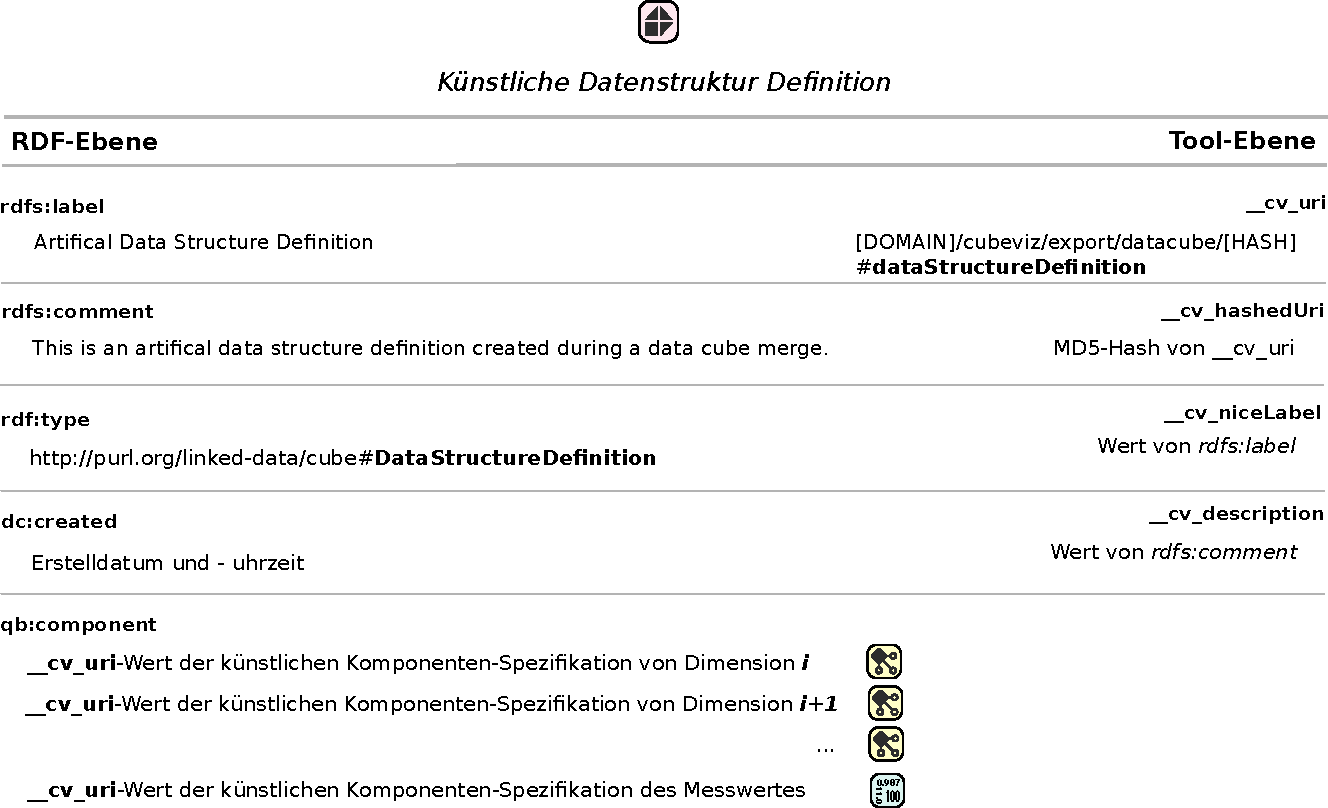
\includegraphics[width=15cm]{MergedDataCube/DataStructureDefinition.pdf}
    \caption{Illustration der Bestandteile einer künstlichen Datenstruktur Definition.}
    \label{fig:MergedDataCube_DataStructureDefinition}
\end{figure}


%
% SSS
%
\subsubsection{Zusammenführung der Beobachtungspunkte aus den Datensätzen}

Es werden die verschiedenen Fälle diskutiert, die bei der Zusammenführung von Beobachtungspunkten aus den Datensätzen eintreten können. Das grobe Vorgehen bei der Zusammenführung ist, die Beobachtungspunkte der jeweiligen Datensätze so zusammenzuführen, dass keiner der Beobachtungspunkte doppelt vorkommt und alle eine gültige Relation zu den künstlichen Dimensionselementen und dem Messwert besitzen. Die Zusammenführung passiert hier im Prinzip genauso wie bei den vorherigen Elementen auch. Es wird ein künstlicher Beobachtungspunkt erstellt, welcher auf einem bestehenden Beobachtungspunkt aus einem der Datensätze basiert. Der Fall möglicher Dopplungen wird später besprochen. 

\newpage
\noindent
Die Schlüssel-Wert-Paare des künstlichen Beobachtungspunktes werden in der folgenden Liste zusammengefasst:

\begin{itemize}

    \item Pendant des künstlichen Beobachtungspunktes wird über den Schlüssel \\\verb|__cv_sourceObservation|  gespeichert

    \item Eigene URI ist nun \verb|[DOMAIN]/cubeviz/export/datacube/[HASH]|\verb|#observation|\textit{\textbf{i}},\\wobei \textit{\textbf{i}} eine fortlaufende Nummer ist
    
    \item Der Wert für den Schlüssel \verb|__cv_hashedUri| wird ebenfalls wieder über einen MD5-Hash der URI generiert
    
    \item Bestehender Wert des Schlüssels \verb|qb:dataSet| wird auf die URI des künstlichen Datensatzes gesetzt
    
    \item Hinzufügen bzw. Erweitern von \verb|dct:source|- und \verb|owl:sameAs|-Schlüsseln, um den Wert der URI des Ausgangsbeobachtungspunktes
    
    \item Hinzufügen bzw. Überschreiben von \verb|dc:created|-Schlüssel mit aktuellem Erstelldatum und -uhrzeit.
    
    \item Hinzufügen von Schlüssel \verb|__cv_sourceDataset|, um das JSON-Objekt des Datensatzes des Ausgangsbeobachtungspunktes zu speichern
    
\end{itemize}

\noindent
Es kann der Fall eintreten,\com{Dopplungen} dass sich die gleichen Beobachtungspunkte in den beiden Datensätzen befinden. Hierbei gilt wie bisher, dass eine gleiche URI als Grund gesehen wird, zwei Elemente als gleich zu betrachten (\textit{F-70})\com{Anforderung \\ F-70, S. \pageref{req:F70}}\label{req:F70source}. Tritt dieser Fall ein, so wird die Erstellung des künstlichen Beobachtungspunktes etwas abgewandelt. Dieser soll zum einen einen ungültigen Messwert verwenden, im JSON-Format ist NaN zu benutzen und zum anderen Relationen auf RDF- und Tool-Ebene zu den Ausgangsbeobachtungspunkten besitzen. Der Grund für die Nutzung eines ungültigen Messwertes liegt darin, zu verhindern, dass etwa Tools wie CubeViz später einfach die Beobachtungspunkte wie normale behandeln, vorausgesetzt sie überprüfen vor der Nutzung die Messwerte. Doch diese Beobachtungspunkte sind nicht normal, denn sie besitzen einen uneindeutigen Messwert, weil sie auf zwei anderen Beobachtungspunkten basieren. In der späteren Behandlung dieses Aspekts soll dem Betrachter diese Situation in ausreichender Form dargelegt werden. Zudem soll er die Möglichkeit haben, die Ausgangsbeobachtungspunkte anzuschauen. 

Ebenfalls als Dopplung\com{Weitere \\Fälle} können zwei Beobachtungspunkte aus verschiedenen Datensätzen angesehen werden, wenn:

\begin{itemize}

    \item ... es zwischen ihnen eine \textbf{sameAs}-Beziehung gibt. 
    
    \item ... sich beide Datensätze jeweils die gleichen Dimensionen teilen und die beiden Beobachtungspunkte jeweils die gleichen Dimensionselemente nutzen. In diesem Fall wären sie jeweils innerhalb ihrer Datensätze eindeutig und zusammen treten sie in Konflikt. 

\end{itemize}

\noindent
Diese Liste soll zwei weitere Möglichkeiten für Dopplungen aufzeigen. Im Rahmen dieses Modells wird nur gefordert, dass der Fall mit der gleichen URI abgedeckt wird. Die beiden anderen Fälle aus der Liste werden als optional angesehen. Die Behandlung mindestens eines Falles wird als notwendig erachtet, um die Semantik innerhalb der Beobachtungspunkte zu wahren. Dabei liegt der Fokus auf einer exemplarischen Behandlung des Falls mit der gleichen URI. Denn die beiden anderen Fälle sind im Hinblick auf eine mögliche Implementierung in CubeViz zu umfangreich, weshalb der einfachere erste Fall gewählt wurde.



%
% SS
%
\subsection{Anforderungen und Spezifikation}
\label{sec:subsectionRequirementsAndSpecification}

Im ersten Teil des Kapitel \ref{sec:sectionCreatingMashup} wurde sehr ausführlich über das Modell zur Zusammenführung von zwei Datensätzen geschrieben. In den verschiedenen Unterkapiteln wurde dazu eine Konkretisierung bzw. Interpretation der DataCube-Elemente durchgeführt und danach eine Reihe von Anforderungen formuliert, welche nun in diesem Kapitel erneut aufgegriffen werden. Es wird im Folgenden darum gehen, alle nötigen Anforderungen zu definieren. Dazu eine kurze Liste der Unterkapitel:

\begin{itemize}
    
    \item \nameref{sec:chapterRequirementsModel} (\ref{sec:chapterRequirementsModel})

    \item \nameref{sec:chapterRequirementsLegend} (\ref{sec:chapterRequirementsLegend})
    
    \item \nameref{sec:chapterRequirementsMergeDatasetsGUI} (\ref{sec:chapterRequirementsMergeDatasetsGUI})

    \item \nameref{sec:chapterRequirementsOptional} (\ref{sec:chapterRequirementsOptional})
    
\end{itemize}

\noindent
Bei den meisten Anforderungen wird auf der rechten Seite ein Vermerk über deren Quelle angegeben. Diese Quelle ist der Textabschnitt, wo die Anforderung das erste Mal erwähnt und diskutiert wurde. Dieser zusätzliche Verweis soll dem Leser ermöglichen, bei Bedarf nochmal nachzulesen, wie bestimmte Anforderungen zustande gekommen sind.


%
% SS
%
\subsubsection{Abgeleitete Anforderungen und Spezifikation aus dem Modell}
\label{sec:chapterRequirementsModel}

Aus dem Grundlagenkapitel sowie dem Unterkapitel über das Modell der Zusammenführung von Datensätzen folgen eine Reihe von Anforderungen. Diese Anforderungen werden nachfolgend erläutert und sie gelten übergreifend für verschiedene Bereiche von CubeViz. Im Implementierungskapitel werden sie jeweils im Kontext der jeweiligen Programmteile betrachtet.

%
% Req
%
\label{req:F10}
\req{/F-10/ Wiedererkennbarkeit des Originals}
{Die \com{Vgl. S. \pageref{req:F10source}}während der Zusammenführung genutzten JSON-Objekte müssen später wieder vollständig ersichtlich sein. Dies soll durch eine Referenzierung auf RDF- und Tool-Ebene geschehen. Dazu müssen sowohl die URI's der Elemente, als auch deren JSON-Pendants referenziert werden.}

\noindent
Die Anforderung \textit{F-10} ist im Rahmen dieser Arbeit sehr wichtig und taucht auch als Referenz bei anderen Anforderungen auf. Sie spiegelt das vorgestellte \nameref{sec:MashupPrinciple-Original} wider und bedeutet, dass man die bei der Exploration von statistischen Daten immer eventuell zugrundeliegende Originaldaten ermitteln kann.


%
% Req
%
\label{req:F20}
\req{/F-20/ Gleichheit zweier Ressourcen}
{Zwei\com{Vgl. S. \pageref{req:F20source}} Ressourcen sind als gleich anzusehen, wenn sie die gleiche URI haben oder durch eine sameAs-Beziehung miteinander verbunden sind. Der Begriff gleich bedeutet hier, dass diese beiden Elemente die gleiche Entität bezeichnen.}

%
% Req
%
\label{req:F30}
\req{/F-30/ Kein Rückschluss auf Gleichheit}
{Teilen\com{Vgl. S. \pageref{req:F30source}} sich zwei ungleiche DataCube-Dimensionen, die jeweils aus verschiedenen Datensätzen stammen, eine Menge von Dimensionselementen, so lässt das keine Rückschlüsse auf die Gleichheit der beiden Dimensionen zu. Sie sind weiterhin als ungleich zu betrachten, unabhängig davon, wie viele Dimensionselemente sie sich teilen.}

%
% Req
%
\label{req:F40}
\req{\com{Vgl. S. \pageref{req:F40source}\\}/F-40/ Eigenschaften der DataCube-JSON-Objekte permanent ersichtlich}
{\com{Referenziert \\ F-10}Die Schlüssel-Wert-Paare der JSON-Objekte, die die DataCube-Elemente repräsentieren, müssen in adäquater Form präsentiert werden, damit der Benutzer sie bei Bedarf anschauen kann.}

%
% Req
%
\label{req:F50}
\req{/F-50/ Künstliche Elemente sind valide DataCube-Elemente}
{Alle\com{Vgl. S. \pageref{req:F50source}} während der Zusammenführung zweier DataCube-Datensätze erstellten künstlichen Elemente müssen valide DataCube-Elemente sein, das heißt, dass sie den in der DataCube-Spezifikation aufgeführten Check-Constraints genügen. (Datenkonsistenz)}

%
% Req
%
\label{req:F60}
\req{/F-60/ Zusammenführung bei mindestens einer gemeinsamen Dimension}
{\com{Vgl. S. \pageref{req:F60source}}Die Zusammenführung von zwei DataCube-Datensätzen ist nur möglich, wenn beide jeweils mindestens eine Dimension besitzen, die es in beiden Datensätzen gibt.}

%
% Req
%
\label{req:F70}
\req{/F-70/ Behandlung doppelter Beobachtungspunkte}
{Doppelte\com{Vgl. S. \pageref{req:F70source}} Beobachtungspunkte liegen vor, wenn es zwei Beobachtungspunkte mit der gleichen URI gibt. Tritt dieser Fall ein, dann soll der Messwert des künstlichen Beobachtungspunktes auf NaN gesetzt werden und die beiden Beobachtungspunkte sollen als Referenzen sowohl über deren URI als auch deren JSON-Objekte selbst an den künstlichen Beobachtungspunkt angehängt werden.}

%
% Req
%
\label{req:F80}
\req{/F-80/ Messwerte sind reelle Zahlen}
{Die\com{Vgl. S. \pageref{req:F80source}} den Beobachtungspunkten zugeordneten Messwerten liegen als reelle Zahlen vor. Aus diesem Grund sind keine weiteren Typ-Prüfungen notwendig.}

%
% Req
%
\label{req:F90}
\req{/F-90/ Zusammenführung von genau zwei Datensätzen}
{Es\com{Vgl. S. \pageref{req:F90source}} sollen bei einer Zusammenführung genau zwei Datensätze genutzt werden.}

%
% Req
%
\label{req:F100}
\req{/F-100/ Zusammenführung muss analog dem vorgestellten Modell geschehen}
{Das Modell zur Zusammenführung zweier Datensätze soll so umgesetzt werden wie beschrieben. Das schließt alle zugehörigen Anforderungen mit ein.}

\noindent
Im Kapitel \ref{sec:chapterModelMergeDatasets}\com{Kapitel \ref{sec:chapterModelMergeDatasets} \\ S. \pageref{sec:chapterModelMergeDatasets}} wurde das Modell detailliert vorgestellt.

%
% SS
%
\subsubsection{Die Benutzeroberfläche der Legende von CubeViz}
\label{sec:chapterRequirementsLegend}

Die folgenden Anforderungen beschreiben eine Reihe von Anpassungen an der Legende, um die drei vorgestellten Anwendungsfälle besser zu unterstützen, mit dem Ziel, die Legende zu einem zentralen Anlaufpunkt für die Exploration der Beobachtungspunkte zu machen. 

%
% Req
%
\label{req:F200}
\req{/F-200/ Auf- und absteigende Sortierung der Beobachtungspunkte}
{Die\com{Vgl. S. \pageref{req:F200source}\\} Benutzeroberfläche muss eine auf- und absteigende Sortierung der Beobachtungspunkte basierend auf den Eigenschaften ermöglichen. Dazu gehört sowohl die auf- und absteigende Sortierung nach den zugeordneten Dimensionselementen als auch nach den Messwerten.}

%
% Req
%
\label{req:F210}
\req{\com{Vgl. S. \pageref{req:F210source}\\}/F-210/ Anzeige aller Schlüssel-Wert-Paare der DataCube-Elemente}
{\com{Referenziert \\ F-10}Der Benutzer muss bei Bedarf in der Legende alle Schlüssel-Wert-Paare der Datenstruktur Definition, des Datensatzes, des Messwertes und, wenn ausgewählt, der Maßeinheit betrachten können.}

%
% Req
%
\label{req:F220}
\req{/F-220/ Anzeige doppelter Beobachtungspunkte}
{\com{Referenziert \\ F-70}Doppelte Beobachtungspunkte sollen so präsentiert werden, dass klar wird, dass es keinen eindeutigen Messwert gibt und welche Originaldaten genutzt wurden. Letzterer Punkt beinhaltet alle Schlüssel-Wert-Paare der jeweiligen Beobachtungspunkte.}

%
% Req
%
\label{req:F230}
\req{/F-230/ Messwerte einzeln veränderbar}
{Der\com{Vgl. S. \pageref{req:F230source}} Benutzer muss die Möglichkeit besitzen, während der Exploration und dem Browsing der Beobachtungspunkte, deren Messwerte einzeln anzupassen.}

%
% Req
%
\label{req:F240}
\req{\com{Vgl. S. \pageref{req:F240source}}/F-240/ Originalwerte von Messwerten müssen permanent ersichtlich sein}
{\com{Referenziert \\ F-10}Wurden Messwerte verändert, so muss es trotzdem für den Benutzer ständig ersichtlich sein, um welchen Originalwert es sich handelte.}


%
% SS
%
\subsubsection{Die Oberfläche zur Zusammenführung von zwei Datensätzen}
\label{sec:chapterRequirementsMergeDatasetsGUI}

Aus dem entwickelten Modell von Kapitel \ref{sec:chapterModelMergeDatasets}\com{Kapitel \ref{sec:chapterModelMergeDatasets} \\ S. \pageref{sec:chapterModelMergeDatasets}} zur Zusammenführung von zwei Datensätzen werden nun eine Reihe von Anforderungen abgeleitet, welche als Fundament für eine Benutzeroberfläche sowie damit zusammenhängende Funktionen dienen sollen. Die Begrifflichkeiten orientieren sich dabei sowohl am DataCube-Vokabular als auch an den verwendeten Begriffen im OntoWiki. Der Anwendungsfall über den Vergleich von Datensätzen wird durch die folgenden Anforderungen weitgehend abgedeckt. Der Anspruch galt hier nicht der Vollständigkeit, sondern einem funktionsfähigen Ansatz, welcher eine Reihe von Aspekten bereithält. So geht es nicht ausschließlich um die Zusammenführung der Datensätze, sondern auch um die Anpassung der Messwerte oder die Selektion von zu nutzenden Beobachtungspunkten.

\newpage
\noindent
Neben dem angesprochenen Anwendungsfall wird durch diese Anforderungen hier auch die kollaborative Zusammenarbeit mithilfe von CubeViz verbessert, z.B. sowohl aufgrund der bereitgestellten Statistiken über Datensätze als auch der unterschiedlichen Zugänge zu den zusammengeführten Datensätzen.

 
%
% Req
%
\label{req:F300}
\req{/F-300/ Erst Modell-Auswahl, danach Datensatz-Auswahl}
{Der Benutzer muss die Möglichkeit haben, aus den verfügbaren Modellen von OntoWiki eines auszuwählen. Danach muss er eine Liste der darin enthaltenen Datensätze erhalten, sofern welche vorhanden sind.}

\noindent
Anmerkung: Modelle werden in OntoWiki auch als Ontologie oder Wissensbasis bezeichnet.

%
% Req
%
\label{req:F301}
\req{/F-301/ Meldung über nicht vorhandene Datensätze}
{Wurde ein Modell ausgewählt, welches keine validen DataCube-Datensätze enthält, soll eine entsprechende Meldung an den Benutzer erfolgen.}

\noindent
Die Anforderungen /F-300/ und /F-301/ sollen nahe beieinanderliegende Bereiche der Benutzeroberfläche nutzen.


%
% Req
%
\label{req:F302}
\req{/F-302/ Keine gleichen Dimensionen gefunden}
{Wurden\com{Referenziert \\ F-20, F-60} keine gleichen Dimensionen gefunden, so ist eine entsprechende Meldung auszugeben und die Zusammenführung zu stoppen.}

%
% Req
%
\label{req:F310}
\req{/F-310/ Statistische Informationen über die Datensätze}
{Eine Übersicht über die DataCube-Informationen eines ausgewählten Datensatzes soll die Anzahl der Dimensionen, Dimensionselemente, Messwerte, Attribute, Schnitte und Beobachtungspunkte enthalten.}

%
% Req
%
\label{req:F320}
\req{/F-320/ Statistische Informationen über die Messwerte}
{Eine detaillierte Übersicht über statistische Informationen der Messwerte eines Datensatzes soll folgende Werte enthalten: Minimum- und Maximalwert, Me-dian, Durchschnittswert, Varianz und Standardabweichung.}

%
% Req
%
\label{req:F330}
\req{/F-330/ Anzeige ungleicher und gleicher Dimensionen mit ihren Elementen}
{Dem Benutzer sollen alle ungleichen und gleichen Dimensionen angezeigt werden, mit Titel und Beschreibung, sofern vorhanden. Bei den gleichen Dimensionen sollen zudem die Dimensionselemente angezeigt werden, die in beiden Dimensionen verwendet werden. Für ungleiche und gleiche Dimensionen soll zudem noch die Anzahl der gleichen und ungleichen Dimensionselemente angezeigt werden.}

\noindent
Die Anforderungen \emph{F-310, F-320} und \emph{F-330} sollen nahe beieinanderliegende Bereiche der Benutzeroberfläche nutzen. Sie fassen allgemeine Informationen über die ausgewählten Datensätze zusammen und gehören damit zusammen.

%
% Req
%
\label{req:F340}
\req{/F-340/ Anpassung aller Messwerte eines Datensatzes (Normalisierung)}
{Es\com{Vgl. S. \pageref{req:F340source}} muss eine Eingabemaske geben, wo der Benutzer eine Formel eingeben kann, wodurch er alle Messwerte eines Datensatzes anpassen kann. Die Formel muss die Grundrechenarten akzeptieren sowie die folgenden Funktionen unterstützen: Natürlicher Logarithmus, Quadratwurzel, Sinus, Kosinus, Tangens sowie Arkussinus, -kosinus und -tangens.}

%
% Req
%
\label{req:F350}
\req{/F-350/ Auswahl der Beobachtungspunkte}
{Die Auswahl der Beobachtungspunkte soll durch den Benutzer getroffen werden. Dafür soll er drei Auswahlmöglichkeiten bekommen: Zunächst sollen alle Beobachtungspunkte genutzt werden können. Die zweite Möglichkeit liegt in der Nutzung der Beobachtungspunkte, welche Dimensionselemente benutzen, die in beiden Datensätzen vorhanden sind. Und die dritte und letzte Möglichkeit ist die Auswahl der Beobachtungspunkte mit Dimensionselementen, welche es nur in einem der Datensätze gibt.}

%
% Req
%
\label{req:F360}
\req{/F-360/ JSON-Objekt für künstlichen Datensatz}
{Nach\com{Vgl. S. \pageref{req:F360source}} der Auswahl der Datensätze soll automatisiert ein künstlicher Datensatz erstellt werden. Dieser Datensatz und all seine DataCube-Elemente sollen jeweils durch ein JSON-Objekt repräsentiert werden. Das JSON-Objekt des Datensatzes wird genauso wie bei CubeViz im ObjektCache von Erfurt abgelegt.}

%
% Req
%
\label{req:F370}
\req{/F-370/ Generierung eines eindeutigen Links}
{\com{Referenziert \\ F-360}Der erzeugte künstliche Datensatz muss über einen eindeutigen Link innerhalb von CubeViz visualisiert werden können. Der Link enthält dazu neben einer möglichen Modell- und ServiceUrl-Auswahl, einen Daten- und UI-Hash. Der Daten-Hash muss dem Namen der JSON-Datei entsprechen, welche die JSON-Repräsentation des künstlichen Datensatzes enthält.}

%
% Req
%
\label{req:F380}
\req{/F-380/ Bereitstellung verschiedener Visualisierungen}
{\com{Referenziert \\ F-370}Es soll dem Benutzer eine Liste an verschiedenen Visualisierungen angeboten werden, über die er den erstellten künstlichen Datensatz betrachten kann. Für die Generierung der Liste soll die bereits in CubeViz existierende Funktionalität, zur Auswahl adäquater Visualisierungen für einen gegebenen Datensatz, wiederverwendet werden.}

%
% Req
%
\label{req:F390}
\req{/F-390/ Wiederverwendbarkeit und Deferenzierbarkeit zusammengeführter Datensätze}
{Die zusammengeführten Datensätze, die basierend auf dem Modell aus Kapitel \ref{sec:sectionCreatingMashup} entstanden sind, müssen dereferenzierbar sein. Weiterhin sollen alle enthaltenen Elemente (Datenstruktur Definition, die Komponenten-Spezifikationen und die Beobachtungspunkte)
jeweils eine dereferenzierbare URI verwenden.}

%
% 
%
\subsubsection{Optionale Anforderungen}
\label{sec:chapterRequirementsOptional}

Die folgenden Anforderungen werden als nützlich, aber optional angesehen.

%
% Req
%
\label{req:F400}
\req{/F-400/ Anker in der Legende}
{Die Meta-Daten sollen in der Legende über HTML-Anker miteinander verbunden werden, so dass man innerhalb der Legende navigieren kann ohne dass die Seite neu lädt.}


%
% Req
%
\label{req:F410}
\req{/F-410/ Anzeige genutzter und vorhandener Dimensionselemente}
{Im Tabellenkopf der Liste mit den Beobachtungspunkten soll für jede Dimension angezeigt werden, wie viele Dimensionselemente jeweils in den Beobachtungspunkten genutzt werden und wie viele es insgesamt in der Dimension gibt.}


%
% Req
%
\label{req:F420}
\req{/F-420/ Änderungsverlauf geänderter Messwerte}
{Ein Änderungsverlauf\com{Referenziert \\ F-230} soll an geeigneter Stelle in der Benutzeroberfläche dem Benutzer darüber Auskunft geben, wann die Messwerte von welchen Beobachtungspunkten geändert wurden.}

%
% Req
%
\label{req:F430}
\req{/F-430/ Clusterbildung der Messwerte}
{Über die Bildung von Clustern aus den Messwerten der ausgewählten Beobachtungspunkte eines zusammengeführten Datensatzes soll dem Benutzer ein alternativer Zugang zu den statistischen Daten gegeben werden. Neben der reinen Auflistung soll eine adäquate Visualisierung genutzt werden.}


%
% Req
%
\label{req:F440}
\req{/F-440/ Export geänderter Messwerte}
{Falls\com{Referenziert \\ F-230, F-420} Messwerte innerhalb der Legende vom Benutzer geändert wurden, so sollen diese auch Teil des Exports sein.}

\noindent
Für die Anforderungen \textit{F-420}\footnote{\url{https://github.com/AKSW/cubeviz.ontowiki/issues/182}} und \textit{F-440}\footnote{\url{https://github.com/AKSW/cubeviz.ontowiki/issues/183}} wurde jeweils ein eigener Feature-Request auf GitHub erstellt, da diese im Rahmen der Arbeit nicht implementiert werden. 

%
% SSS
% 
\newpage
\subsubsection{Die Anforderungen im Überblick}

Die folgenden Tabellen bieten noch einmal eine Übersicht aller aufgestellten Anforderungen. 
Ihre Spalten im Überblick:

\begin{itemize}
	\item \textit{ID} -- Die erste Spalte enthält die Bezeichnung der Anforderung
	
	\item \textit{Titel} -- Dahinter verbirgt sich Titel der jeweiligen Anforderung
	
	\item \textit{Def.} -- Die jeweiligen Zellen enthalten eine Seitenangabe, wo die jeweilige Anforderung definiert wurde
	
	\item \textit{Vgl.} -- Die jeweiligen Zellen enthalten eine Seitenangabe, wo die jeweilige Anforderung das erste Mal eingeführt und diskutiert wurde
	
	\item \textit{Ref.} -- Angabe von referenzierten Anforderungen
	
\end{itemize}

\begin{table}[h!]
\small
\begin{tabularx}{400pt}{ p{1cm} p{7.6cm} p{1.1cm} p{0.9cm} p{1.6cm} }
\rotatebox{30}{\textbf{ID}} &
\rotatebox{30}{\textbf{Titel}} &
\rotatebox{30}{\textbf{Def.}} &
\rotatebox{30}{\textbf{Vgl.}} &
\rotatebox{30}{\textbf{Ref.}} 
\\
\toprule 
    \\F-10 & Originaldaten müssen immer ersichtlich sein & S. \pageref{req:F10} & S. \pageref{req:F10source} & \\
    \\F-20 & Gleichheit zweier Ressourcen & S. \pageref{req:F20} & S. \pageref{req:F20source} & \\

    \\F-30 & Kein Rückschluss auf Gleichheit & S. \pageref{req:F30} & S. \pageref{req:F30source} & \\

    \\F-40 & Eigenschaften der DataCube-JSON-Objekte permanent ersichtlich & S. \pageref{req:F40} & S. \pageref{req:F40source} & F-10 \\

    \\ F-50 & Künstliche Elemente sind valide DataCube-Elemente & S. \pageref{req:F50} & S. \pageref{req:F50source} & \\

    \\ F-60 & Zusammenführung bei mindestens einer gemeinsamen Dimension & S. \pageref{req:F60} & S. \pageref{req:F60source} & \\

    \\ F-70 & Behandlung doppelter Beobachtungspunkte & S. \pageref{req:F70} & S. \pageref{req:F70source} & \\

    \\ F-80 & Messwerte sind reelle Zahlen & S. \pageref{req:F80} & S. \pageref{req:F80source} & \\
        
    \\ F-90 & Zusammenführung von genau zwei Datensätzen & S. \pageref{req:F90} & & \\
    
    \\ F-100 & Zusammenführung muss analog dem vorgestellten Modell geschehen & S. \pageref{req:F100} & & \\\\

\bottomrule
    
\end{tabularx}
\caption{Anforderungen für bereichsübergreifende Anpassungen.}
\label{tab:requirementsOverall}
\end{table}

%-----------------------------------------------------
% LEGENDE

\begin{table}[h]
\small
\begin{tabularx}{400pt}{ p{1cm} p{7.6cm} p{1.1cm} p{0.9cm} p{1.6cm} }
\rotatebox{30}{\textbf{ID}} &
\rotatebox{30}{\textbf{Titel}} &
\rotatebox{30}{\textbf{Def.}} &
\rotatebox{30}{\textbf{Vgl.}} &
\rotatebox{30}{\textbf{Ref.}} 
\\
\toprule 
    \\ F-200 & Auf- und absteigende Sortierung der Beobachtungspunkte & S. \pageref{req:F200} & S. \pageref{req:F200source} & \\
           
    \\ F-210 & Anzeige aller Schlüssel-Wert-Paare der DataCube-Elemente & S. \pageref{req:F210} & S. \pageref{req:F210source} & F-10 \\

    \\ F-220 & Anzeige doppelter Beobachtungspunkte & S. \pageref{req:F220} & & F-70 \\

    \\ F-230 & Messwerte einzeln veränderbar & S. \pageref{req:F230} & S. \pageref{req:F230source} & \\

    \\ F-240 & Originalwerte von Messwerten müssen permanent ersichtlich sein & S. \pageref{req:F240} & S. \pageref{req:F240source} & F-10 \\\\

\bottomrule
\end{tabularx}
\caption{Anforderungen für Anpassungen an Legende.}
\label{tab:requirementsToLegend}
\end{table}

%-----------------------------------------------------
% Compare-Action GUI
\begin{table}[htop!]
\small
\begin{tabularx}{400pt}{ p{1cm} p{7.6cm} p{1.1cm} p{0.9cm} p{1.6cm} }
\rotatebox{30}{\textbf{ID}} &
\rotatebox{30}{\textbf{Titel}} &
\rotatebox{30}{\textbf{Def.}} &
\rotatebox{30}{\textbf{Vgl.}} &
\rotatebox{30}{\textbf{Ref.}} 
\\
\toprule
    \\ F-300 & Erst Modell-Auswahl, danach Datensatz-Auswahl & S. \pageref{req:F300} & & \\
 
    \\ F-301 & Meldung über nicht vorhandene Datensätze & S. \pageref{req:F301} & & F-300 \\
 
    \\ F-302 & Keine gleichen Dimensionen gefunden & S. \pageref{req:F302} & & F-20, F-60 \\
    
    \\ F-310 & Statistische Informationen über die Datensätze & S. \pageref{req:F310} & & \\
    
    \\ F-320 & Statistische Informationen über die Messwerte & S. \pageref{req:F320} & & \\
           
    \\ F-330 & Anzeige ungleicher und gleicher Dimensionen sowie ihrer Elemente & S. \pageref{req:F330} & & \\
           
    \\ F-340 & Anpassung aller Messwerte eines Datensatzes & S. \pageref{req:F340} & S. \pageref{req:F340source} & \\
   
    \\ F-350 & Auswahl der Beobachtungspunkte & S. \pageref{req:F350} & S. \pageref{req:F350source} & \\
    
    \\ F-360 & JSON-Objekt für künstlichen Datensatz & S. \pageref{req:F360} & S. \pageref{req:F360source} & \\
    
    \\ F-370 & Generierung eines eindeutigen Links & S. \pageref{req:F370} & & F-360 \\
    
    \\ F-380 & Bereitstellung verschiedener Visualisierungen & S. \pageref{req:F380} & & F-370 \\

    \\ F-390 & Wiederverwendbarkeit und Dereferenzierung zusammengeführter Datensätze & S. \pageref{req:F390} & \\

\bottomrule
\end{tabularx}
\caption{Anforderungen für Oberfläche zur Zusammenführung zweier Datensätze.}
\label{tab:requirementsToUIMergeDatasets}
\end{table}

%
% --------------------------------------------------------------
% Optional Requirements
%
\clearpage
\newpage
\noindent

\begin{table}[h]
\small
\begin{tabularx}{400pt}{ p{1cm} p{7.6cm} p{1.1cm} p{0.9cm} p{1.6cm} }
\rotatebox{30}{\textbf{ID}} &
\rotatebox{30}{\textbf{Titel}} &
\rotatebox{30}{\textbf{Def.}} &
\rotatebox{30}{\textbf{Vgl.}} &
\rotatebox{30}{\textbf{Ref.}} 
\\
\toprule 
    \\ F-400 & Anker in Legende & S. \pageref{req:F400} & & \\

    \\ F-410 & Anzeige genutzter und vorhandener Dimensionselemente & S. \pageref{req:F410} & & \\
    
    \\ F-420 & Änderungsverlauf geänderter Messwerte & S. \pageref{req:F420} & & F-230 \\
    
    \\ F-430 & Clusterbildung der Messwerte & S. \pageref{req:F430} & & \\
    
    \\ F-440 & Export geänderter Messwerte & S. \pageref{req:F440} & & F-230, \mbox{F-420} \\

\bottomrule
\end{tabularx}
\caption{Liste mit optionalen Anforderungen.}
\label{tab:requirementsToLegend}
\end{table}



%
% -------------------------------------------------------------
%
\clearpage
\newpage
\section{Implementierung und Anpassung}
\label{sec:chapterImplemenation}

In diesem Kapitel wird die Implementierung der aufgestellten Anforderungen von Kapitel \ref{sec:subsectionRequirementsAndSpecification} besprochen. Dazu werden die während der Implementierung durchgeführten Anpassungen und Erweiterungen thematisch gruppiert, anstatt einzeln aufgezählt zu werden. Die einzelnen Unterkapitel sind wie folgt:

\begin{itemize}
    \item \nameref{sec:chapterUIMergeDatasets} (\ref{sec:chapterUIMergeDatasets})

    \item \nameref{sec:chapterLegendAdaptions} (\ref{sec:chapterLegendAdaptions})
    
    \item \nameref{sec:chapterVisualizationAdaptions} (\ref{sec:chapterVisualizationAdaptions})
    
    \item \nameref{sec:chapterMiscAdaptions} (\ref{sec:chapterMiscAdaptions})
\end{itemize}

Die Implementierung der einzelnen Anforderungen wurde getrennt vom\com{Branch:\\ comparing} Hauptentwicklungszweig von CubeViz durchgeführt. Dazu wurde der Branch \textit{comparing} angelegt, welche alle oben angesprochenen Commits enthält. Während der Entwicklung wurde nach zeitlichen Abständen immer wieder der Branch \textit{v0.9} in den eigenen Branch überführt, um von den Steigerungen in der Performance zu profitieren. Weitere\com{Anhang \ref{sec:appendixSourceCode} \\ S. \pageref{sec:appendixSourceCode}} Informationen dazu im Anhang \ref{sec:appendixSourceCode}. 

%
% SS
%
\subsection{Oberfläche zur Zusammenführung zweier Datensätze}
\label{sec:chapterUIMergeDatasets}

In diesem Unterkapitel geht es um die Vorstellung einer Oberfläche zur Zusammenführung von zwei Datensätzen und damit der besseren Unterstützung des Anwendungsfalls \nameref{sec:chapterUC3}. Im Rahmen dieser Implementierung wurden nicht nur neue Funktionen und eine eigene Oberfläche entwickelt, sondern auch bestehende Funktionalitäten in CubeViz angepasst. Dies wurde nötig, um weitere Workflows zu ermöglichen, ohne bestehende zu verändern oder gar zu verlieren. Auf den folgenden Seiten werden die einzelnen Teile der Oberfläche und ihrer jeweiligen Funktionen vorgestellt. \\

%
% Abbildung
%
\begin{figure}[h!]
    \centering
    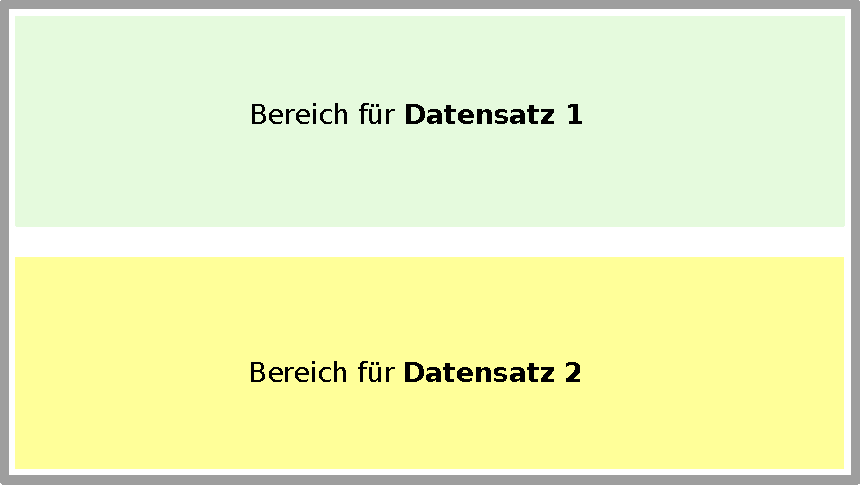
\includegraphics[width=8cm]{UserInterfaceMergeDatasets/UserInterfaceAreas.pdf}
    \caption{Illustration der übereinanderliegende Bereiche der Benutzeroberfläche.}
    \label{fig:UserInterfaceMergeDatasets_UserInterfaceAreas}
\end{figure}

\newpage
\noindent
Im Kapitel \ref{sec:chapterModelMergeDatasets} wurde die These mit den beiden Händen erwähnt. Dabei ging es darum, dass man als Mensch in der Regel seine beiden Hände benutzt um Dinge zu vergleichen, indem man etwas jeweils in die Hand nimmt und untersucht. Dieses Prinzip wird nun auf die Benutzeroberfläche übertragen, siehe Abbildung \ref{fig:UserInterfaceMergeDatasets_UserInterfaceAreas}. Jeder Bereich steht analog für eine Hand und später für einen Datensatz. Vorgegriffen, es kommt später erst zu einer Modell- danach zu einer Datensatzauswahl. Das Modell ist dabei aber sekundär und dient nur als Ausgangspunkt für die Datensatzauswahl. Im Folgenden werden die einzelnen Bereiche der Benutzeroberfläche vorgestellt, wobei die dabei gezeigten Screenshots immer nur für einen Datensatz stehen. Für den zweiten Datensatz gelten die Aussagen analog. 

%
% SSS
%
\subsubsection{Die Modell- und Datensatzauswahl}

%
% Abbildung
%
\begin{figure}[h!]
    \centering
    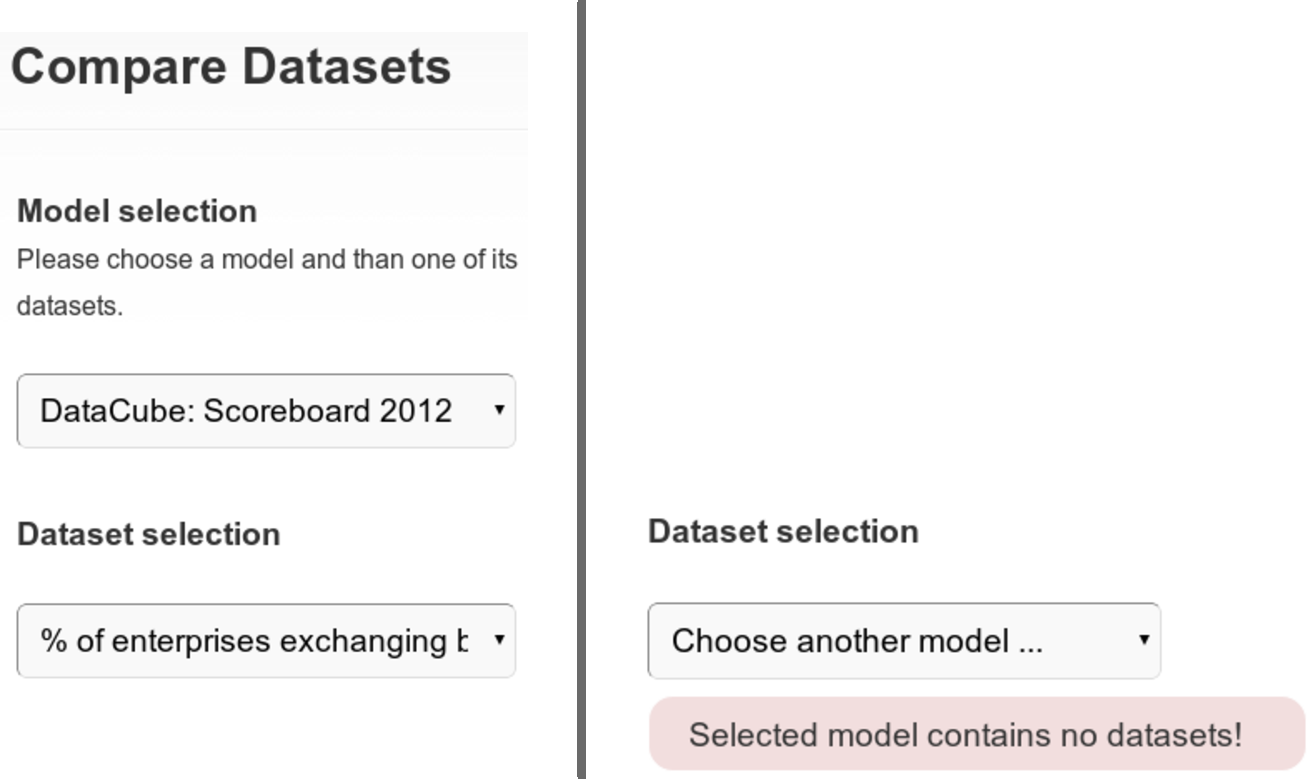
\includegraphics[width=11cm]{UserInterfaceMergeDatasets/ScreenWhileModelDSSelection.pdf}
    \caption{Screenshot zur Modell- und Datensatz-Auswahl.}
    \label{fig:UserInterfaceMergeDatasets_ScreenWhileModelDSSelection}
\end{figure}

Auf der Abbildung \ref{fig:UserInterfaceMergeDatasets_ScreenWhileModelDSSelection} ist ein Screenshot der Benutzeroberfläche für die\com{Anforderungen \\ F-300, S. \pageref{req:F300} \\\\\\ \mbox{F-301, S. \pageref{req:F301}}} Modell- und Datensatz-Auswahl dargestellt. Die Anforderung \textit{F-300} zielt darauf ab, dass der Benutzer nach einer Modellauswahl einen Datensatz auszuwählen hat. Das heißt, unmittelbar nach der Auswahl eines Modells wird darunter eine Liste der enthaltenen Datensätze angezeigt. Sollten keine Datensätze innerhalb des ausgewählten Modells vorhanden sein, so muss eine Meldung darüber ausgegeben werden. Wie so etwas aussieht, kann man auf der rechten Seite der Abbildung \ref{fig:UserInterfaceMergeDatasets_ScreenWhileModelDSSelection} sehen.


%
% SSS
%
\subsubsection{Statistische Informationen über Datensätze und Messwerte}

Nach der Modell- und Datensatzauswahl erfolgt eine Vergrößerung der Benutzer-oberfläche. Direkt neben dem bisher vorgestellten Bereich werden eine Reihe weiterer Bereiche eingeblendet.

%
% Abbildung
%
\newpage
\begin{figure}[h!]
    \centering
    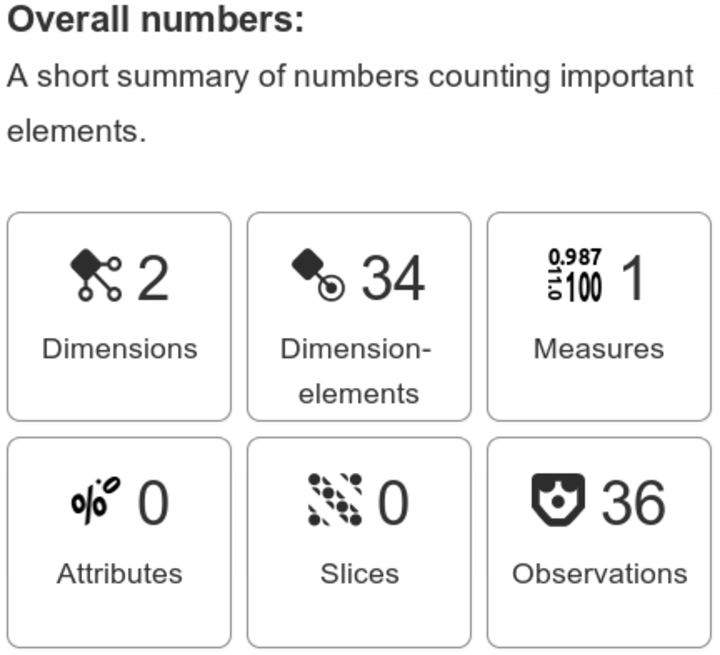
\includegraphics[width=6cm]{UserInterfaceMergeDatasets/ScreenAfterModelDSSelection.pdf}
    \caption{Screenshot mit statistischen Daten über einen Datensatz.}
    \label{fig:UserInterfaceMergeDatasets_ScreenAfterModelDSSelection}
\end{figure}

\noindent
Der erste neue Bereich enthält statistische Informationen\com{Anforderung \\ F-310, S. \pageref{req:F310}} über einen ausgewählten Datensatz. Diese sind die Anzahl der Dimensionen, Dimensionselemente, Messwerte, Maßeinheiten, Schnitte und Beobachtungspunkte. Die jeweiligen Zahlen werden durch ein entsprechendes semicon unterlegt. 

Die neue Funktion \verb|loadNumberOfObservations()|\com{Commit \\579968} wurde zu der TypeScript-Datei \verb|Model/| \\\verb|DataCube/Observation.ts| hinzugefügt, um die Anzahl der Beobachtungspunkte eines Datensatzes zu ermitteln. Sie nutzt die Action \verb|getnumberofobservationsAction()| von \verb|Cube| \verb|vizController.php| um die Anzahl zu bestimmen, wobei sie nur maximal 1000 Stück abfragt. Gibt es mehr davon, wird einfach nur \verb|1000+| angezeigt, um die Datenbank nicht unnötig zu belasten.

Weiterhin wurde die Action \verb|getdatasetsAction()| vom \verb|CubevizController.php| angepasst, so dass man nun für ein gegebenes Modell alle enthaltenen Datensätze abfragen kann, unabhängig der URL einer Datenstruktur Definition.

Die bisher eigenständige Behandlung von Attributen wurde so geändert,\com{Commit \\0c46e4} dass die Action \verb|getcomponentsAction()| von \verb|CubevizController.php| nun auch Attribute abfragen und verwalten kann. Der Grund ist, dass Attribute laut Spezifikation ebenfalls den Komponenten-Spezifikationen zugeordnet sind, aber bisher eigenständig implementiert waren. Auf diese Weise ist es konsistenter.

Mit den aufgezählten Änderungen war es möglich, alle statistischen Informationen über einen Datensatz abzufragen, die von Interesse waren. Man hat sich bei manchen Funktionen dafür entschieden, zuerst alle Elemente einer Art abzufragen und sie danach zu zählen. Bei anderen wiederum, wie beispielsweise bei den Beobachtungspunkten, wurde eine eigene Zählfunktion eingesetzt. Wie bereits erwähnt, soll damit die Datenbank weitestgehend geschont werden.

Die Abbildung \ref{fig:UserInterfaceMergeDatasets_StatisticsAboutMeasureValues} zeigt statistische Informationen über alle Messwerte der empfangenen Beobachtungspunkte eines ausgewählten Datensatzes.\com{Anforderung \\ F-320, S. \pageref{req:F320}} Zu den Informationen zählen der Minimum- und Maximalwert, Median, Mittelwert, die Varianz und die Standardabweichung. Alle bilden jeweils eine Spalte in der Tabelle. 

\newpage
\noindent

%
% Abbildung
%
\begin{figure}[h!]
    \centering
    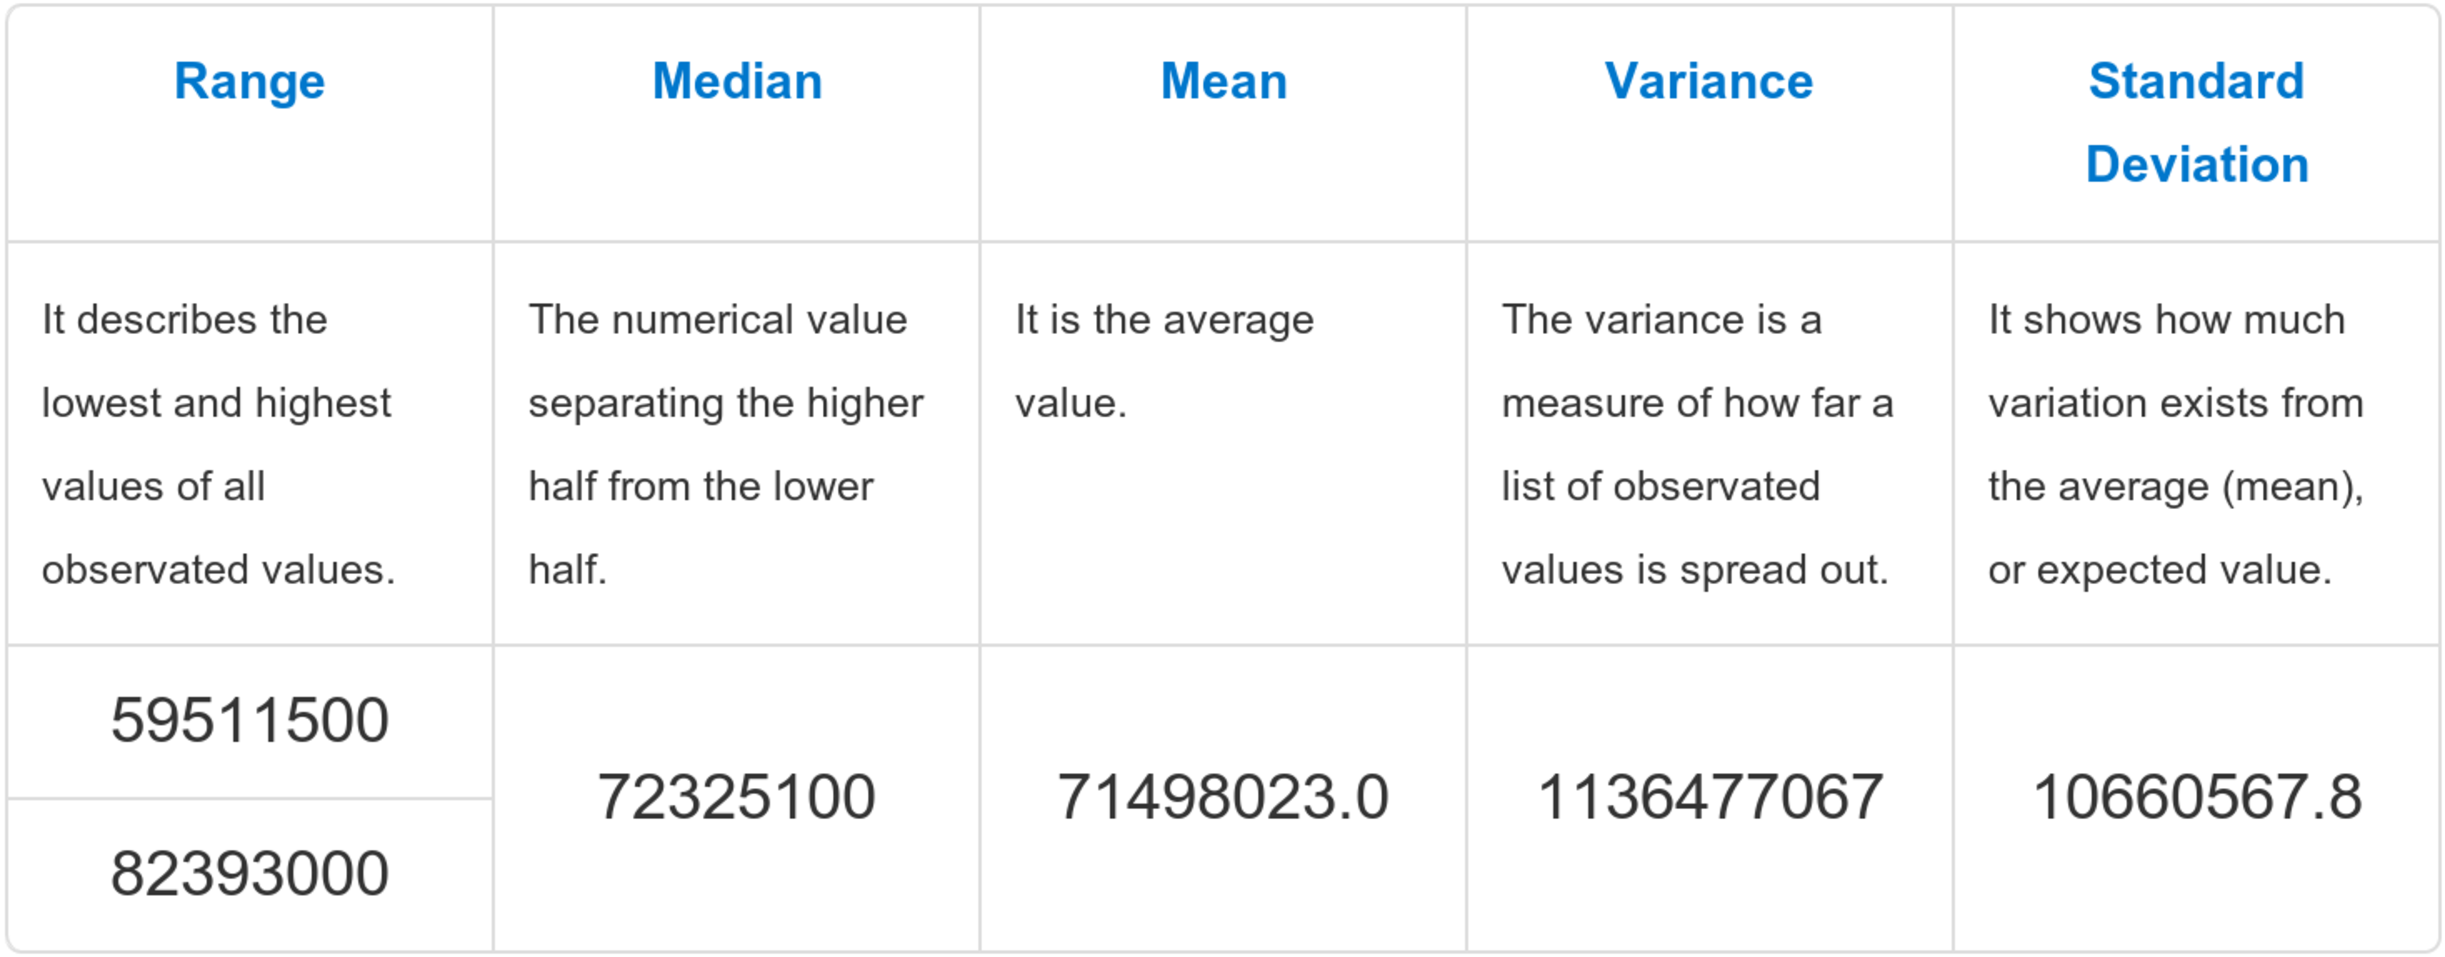
\includegraphics[width=15cm]{UserInterfaceMergeDatasets/StatisticsAboutMeasureValues.pdf}
    \caption{Screenshot mit statistischen Daten über die Werte innerhalb eines Datensatzes.}
    \label{fig:UserInterfaceMergeDatasets_StatisticsAboutMeasureValues}
\end{figure}

\noindent
Auf der Abbildung sind pro Spalte erst der Titel der Information, darunter ein kurzer Beschreibungstext sowie die jeweiligen Werte zu sehen. Der Beschreibungstext soll dem Benutzer einen kurzen Hinweis zu den einzelnen Arten der Informationen zu geben. Die Spaltentitel sind deshalb blau, weil sie Links auf zugehörige Wikipedia-Artikel sind. Dies wurde für den Fall eingerichtet, dass eine statistische Information für den Betrachter unklar ist.

Um statistische Informationen über die Messwerte der Beobachtungspunkte eines Datensatzes zu gewinnen, wurde die JavaScript-Bibliothek \textit{jsStats}\footnote{\url{http://code.google.com/p/jsstats}}\com{jsStats} genutzt. Sie wurde zwar seit 2008 nicht mehr aktualisiert, aber ihre bereitgestellten Funktionen liefern korrekte Werte und sind einfach zu benutzen.

%
% SSS
%
\subsubsection{Übersicht über gleiche und ungleiche Dimensionen}

Nachdem ein Überblick über die ausgewählten Datensätze gegeben wurde, kommen wir nun zur Übersicht über die enthaltenen Dimensionen. Wie auf der Abbildung \ref{fig:UserInterfaceMergeDatasets_DimensionsOverview} zu sehen,\com{Anforderung \\ F-330, S. \pageref{req:F330}} werden die Dimensionen danach aufgeteilt, ob sie gleich sind oder nicht.

Die ungleichen Dimensionen werden zuerst angezeigt, wie auf der Abbildung links zu sehen ist. Es werden eine Dimension namens \verb|country (CS)|, ein leeres Feld, wo ein möglicher Beschreibungstext stehen könnte sowie ganz unten die Anzahl der Dimensionselemente angezeigt. Streng genommen handelt es sich hier um eine Komponenten-Spezifikation, der eine Dimension zugeordnet wurde. Da aber in der Spezifikation auch nur von Dimensionen gesprochen wird, wird dies hier in der Benutzeroberfläche ebenfalls so kommuniziert. Die Datei \verb|typescript/src/View/CompareAction/DimensionOverview.ts| verwaltet den für die Benutzeroberfläche relevanten Bereich.

\newpage

%
% Abbildung
%
\begin{figure}[h!]
    \centering
    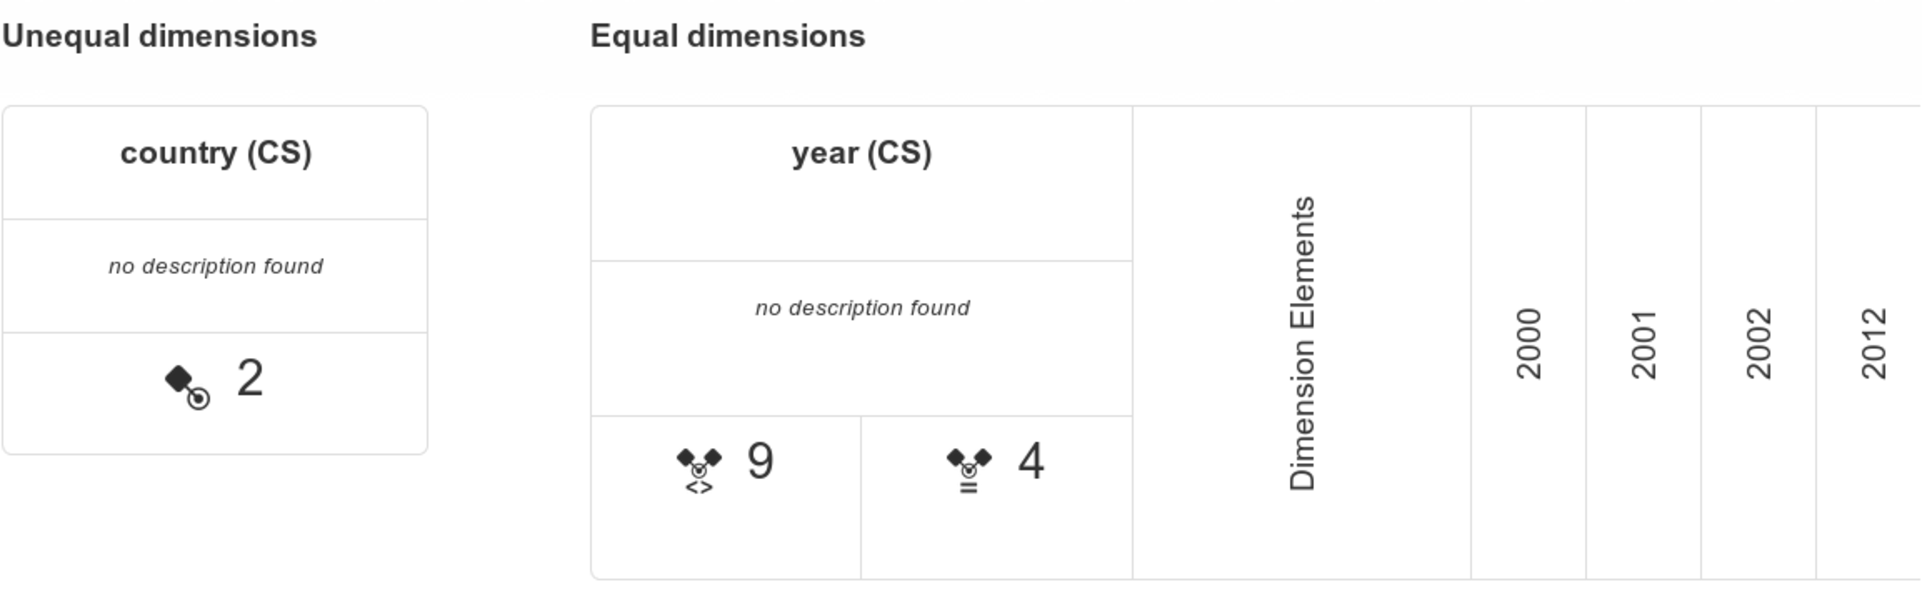
\includegraphics[width=14.3cm]{UserInterfaceMergeDatasets/DimensionsOverview.pdf}
    \caption{Screenshot der Informationen über ungleiche und gleiche Dimensionen.}
    \label{fig:UserInterfaceMergeDatasets_DimensionsOverview}
\end{figure}


%
% SSS
%
\subsubsection{Keine gleichen Dimensionen gefunden}

Tritt der Fall ein, dass keine gleichen Dimensionen gefunden worden sind,\com{Anforderung \\ F-302, S. \pageref{req:F302}} so wird eine entsprechende Meldung ausgegeben und die weitere Verarbeitung gestoppt. Dem Benutzer soll damit klar gemacht werden, dass er die beiden Datensätze nicht zusammenführen kann. Er wird darauf hingewiesen, dass er die ausgewählten Datensätze mit entsprechenden Relationen anreichern muss, um fortfahren zu können. Dafür kann er Programme wie SILK\cite{SILK} verwenden.

%
% SSS
%
\subsubsection{Die Zusammenführung zweier Datensätze}

Nachdem besprochen wurde, wie Cubeviz bei ungleichen Dimensionen vorgeht, soll nun die Zusammenführung zweier Datensätze mit mindestens einem Paar gleicher Dimensionen erläutert werden. Die beiden Datensätze werden vollautomatisiert zerlegt, die jeweiligen Elemente verarbeitet und in einem künstlichen Datensatz zusammenführt. Der Grund für eine vollautomatisierte Vorgehensweise ist, dass der Benutzer nach der Auswahl der Datensätze einen Einstiegspunkt in die Visualisierungen bekommt, ohne erst weitere Einstellungen tätigen zu müssen. Für die Visualisierung und Exploration wird die bestehende Visualisierungskomponente von CubeViz genutzt, doch dazu später mehr. In diesem Unterkapitel wird die prinzipielle Vorgehensweise bei der automatisierten Zusammenführung beschrieben und welche Änderungen damit einhergingen.

Im Rahmen der Implementierung wurde die Funktion \verb|getObservations()| der Datei \verb|classes/DataCube/Query.php| angepasst.\com{Commit \\ 35e326} Sie limitiert die Anzahl der abfragbaren Beobachtungspunkte, um einerseits die Datenmenge bei der Zusammenführung überschaubar zu halten und andererseits die Datenbank nicht unnötig zu belasten. Würde man keine Limitierung nutzen, so bestünde die Gefahr, dass bei der Abfrage einiger Tausend Beobachtungspunkte der Server unter große Last gelegt wird. Denn hinter dieser Menge an Beobachtungspunkten können leicht einige Millionen Tripel stehen. 

Die Funktion \verb|loadAll()| in der Datei \verb|Model/DataCube/Observation.ts| wurde um den Parameter \verb|datasetUri| erweitert\com{Commit \\ 4d1601}. 

\newpage
\noindent
Damit können nun auch alle Beobachtungspunktes eines Datensatzes abgefragt werden. Bisher war es lediglich möglich, sich unter Angabe eines Daten-Hashes die in der zugehörigen Datei abgespeicherten Beobachtungspunkte zu holen.

Die Anforderung \emph{F-390}\com{Anforderung \\ F-390, S. \pageref{req:F390}} verlangt die Wiederverwendbarkeit und Deferenzierbarkeit zusammengeführter Datensätze. Dies war bisher mit CubeViz so nicht möglich. Aus diesem Grund wurde die Export-Funktion erweitert, welche bisher nur zu einem gegebenen Daten-Hash die zugehörigen DataCube-Daten als Datei zurücklieferte. Diese Funktionalität wurde so angepasst\com{Commit \\ 76a4b0}, dass man der Action als Parameter entweder die Zeichenkette \verb|datacube| oder \verb|dataselection| übergibt, wobei nach beiden der Daten-Hash folgen muss. Die Nutzung des Parameters \verb|dataselection| wurde weiterhin für den Visualisierungsbereich von CubeViz verwendet, über den man seine aktuelle Datenselektion exportieren konnte. Der neue Parameter \verb|datacube| hingegen wird für zusammengeführte Datensätze eingesetzt. So haben der zusammengeführte Datensatz und alle in ihm enthaltenen Elemente denselben Namensraum, welcher die Export-URI enthält sowie den \verb|datacube|-Parameter mit dem entsprechenden Hash. Nur nach dem Hash-Zeichen am Ende unterscheiden sich die Elemente, abhängig von ihrer Bezeichnung. Dazu das Schema zur Bildung des Namensraums für diese künstlichen Elemente:

\begin{center}
	Namensraum: \verb|[DOMAIN]/cubeviz/export/datacube/[HASH]|
\end{center}

\noindent
Nach dieser Änderung ist es nun möglich,\com{Commit \\ 93ebed} die URI eines zusammengeführten Datensatzes mit dem Browser aufzurufen und sich die RDF-Turtle direkt anzuschauen oder als Datei herunterzuladen. Man muss hier anmerken, dass die Speicherung der Daten im ObjectCache stattfindet und dieser nicht persistent ist. Zwar muss die Leerung des ObjectCaches manuell durch den Betreiber der Seite durchgeführt werden, aber führt er sie sie einmal durch, verschwinden alle Daten unwiederbringlich und jegliche Links zu zusammengeführten Datensätzen werden ungültig. Dies muss für die künftige Entwicklung berücksichtigt und gewiss verbessert werden.

Im Zusammenhang mit der Erweiterung der Export-Funktionalität wurde eine andere große Änderung durchgeführt. Bisher war es so, dass CubeViz alle Daten, bis auf die Beobachtungspunkte, in Form eines JSON-Objektes im ObjectCache abgelegt hat. Nachdem eine SPARQL-Abfrage gebaut wurde, konnten die betreffenden Beobachtungspunkte aus der Datenbank abgefragt werden. Die Änderung dieses Verhaltens wurde nötig, weil zusammengeführte Datensätze nur als JSON-Objekte in Dateiform im ObjectCache vorliegen und Abfragen der Datenbank keinen Sinn ergeben, weil sich darin keine nutzbaren Daten befinden. Daher wurde der neue Parameter \verb|useObservations| zur Action \verb|savecontenttofile()| von \verb|CubevizController.php| hinzugefügt, welcher CubeViz mitteilt, nur die Beobachtungspunkte der JSON-Daten zu benutzen und nicht die Datenbank abzufragen.


%
% SSS
%
\subsubsection{Eingabemaske zur Normalisierung der Messwerte}

Ist der Benutzer mit der automatisierten Zusammenführung nicht zufrieden, so hat er eine Reihe von Möglichkeiten, das Ergebnis zu verändern. Eine davon ist die Normalisierung der Messwerte. Dabei werden die Messwerte aller Beobachtungspunkte eines Datensatzes über eine vom Benutzer definierte Formel angepasst. Auf diese Weise können Messwerte, die sich auf verschiedenen und weit auseinanderliegenden Skalen befinden, einander angenähert werden. \\


%
% Abbildung
%
\begin{figure}[h!]
    \centering
    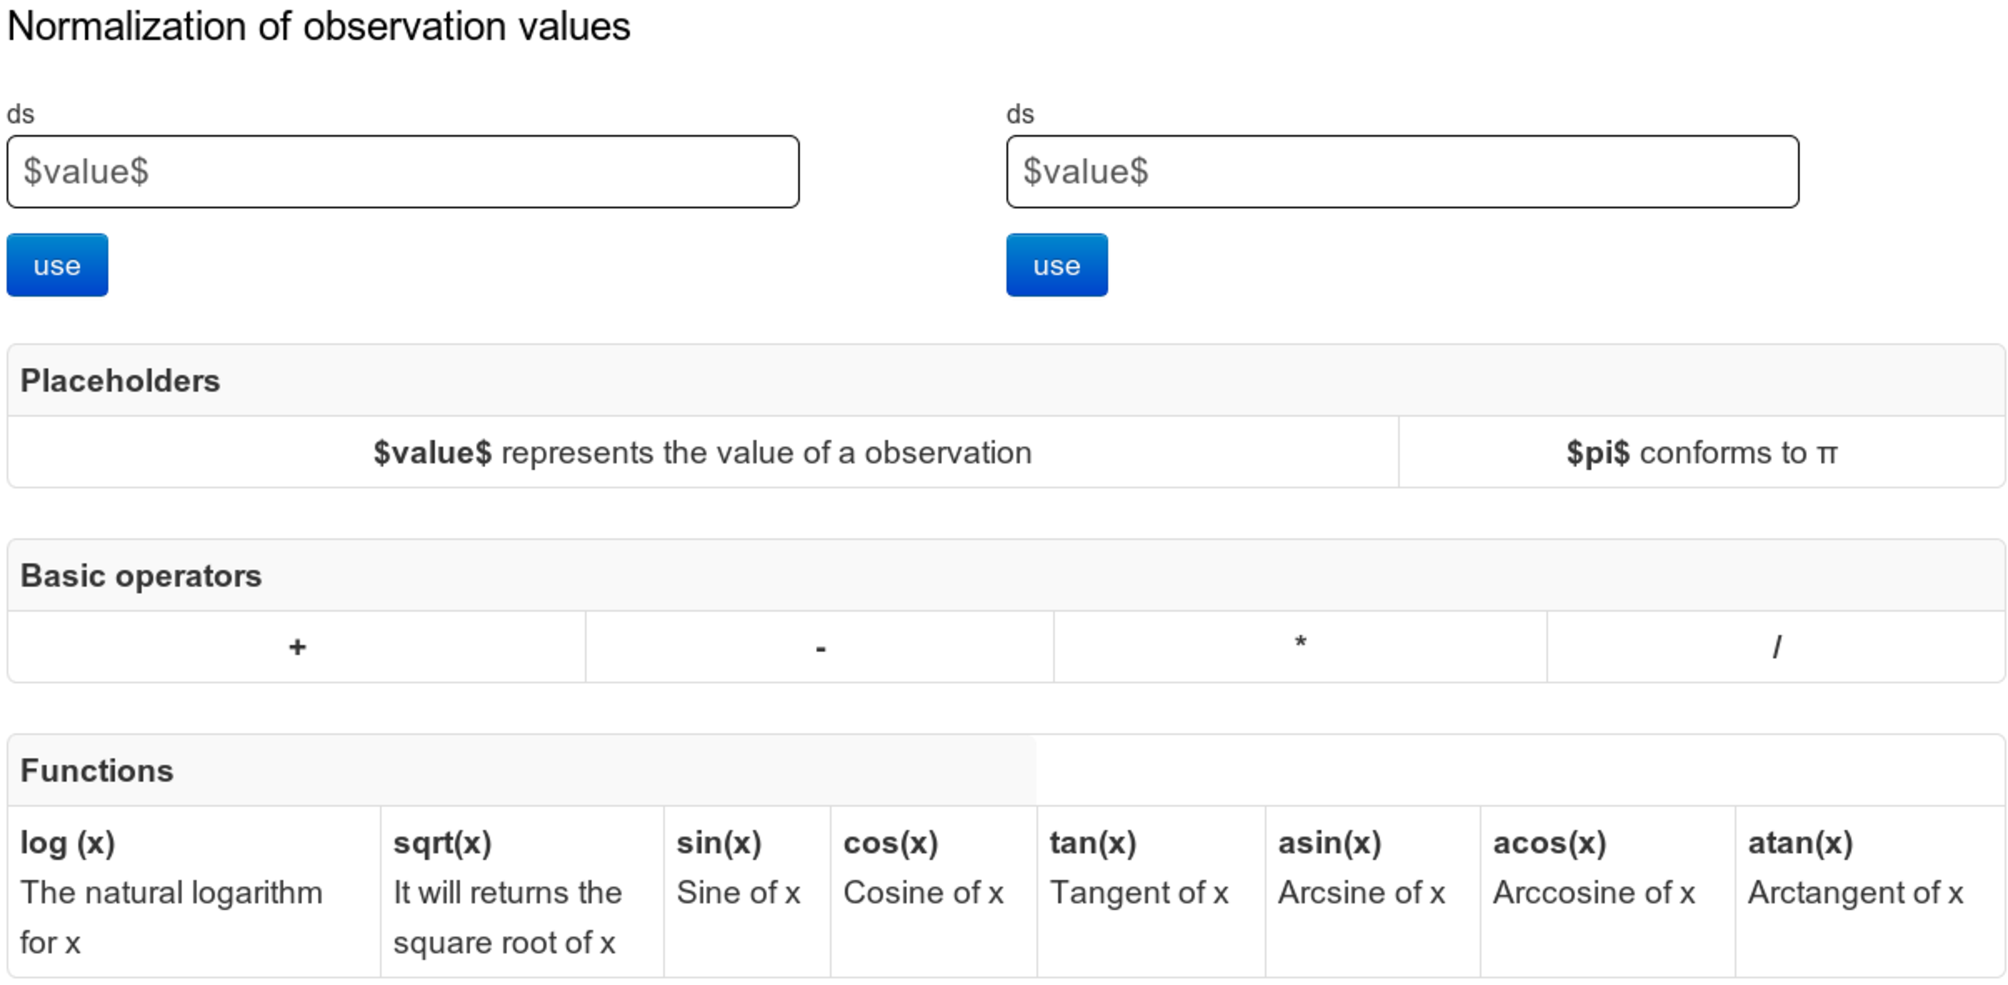
\includegraphics[width=14.3cm]{UserInterfaceMergeDatasets/NormalizationUserInterface.pdf}
    \caption{Screenshot der Eingabemaske der Formel zur Normalisierung der Messwerte.}
    \label{fig:UserInterfaceMergeDatasets_NormalizationUserInterface}
\end{figure}

\noindent
Auf der Abbildung \ref{fig:UserInterfaceMergeDatasets_NormalizationUserInterface} sind zwei Eingabemasken für je einen der ausgewählten Datensätze abgebildet, um deren Messwerte bei Bedarf zu normalisieren. Im oberen Bereich findet man auf der linken Seite ein Eingabefeld für den ersten Datensatz und rechts daneben eines für den zweiten. Eingaben und Änderungen werden erst nach dem Drücken des blauen \textit{use}-Buttons aktiv. Darunter befindet sich eine Übersicht aller verfügbaren Befehle und Platzhalter. Die Platzhalter stehen einmal für einen Wert eines Beobachtungspunktes und dann für Pi. Neben den vier Rechenoperationen, werden auch eine Reihe algebraischen und trigonometrischen Funktionen unterstützt,\com{Anforderung \\ F-340, S. \pageref{req:F340}} wie im Beschreibungstext der Anforderung \textit{F-340} verlangt. Nach dem Drücken des use-Buttons wird die Zusammenführung noch einmal mit angepassten Messwerten durchgeführt. 


%
% SSS
%
\subsubsection{Auswahl der Beobachtungspunkte anhand der Dimensionselemente}

%
% Abbildung
%
\begin{figure}[h!]
    \centering
    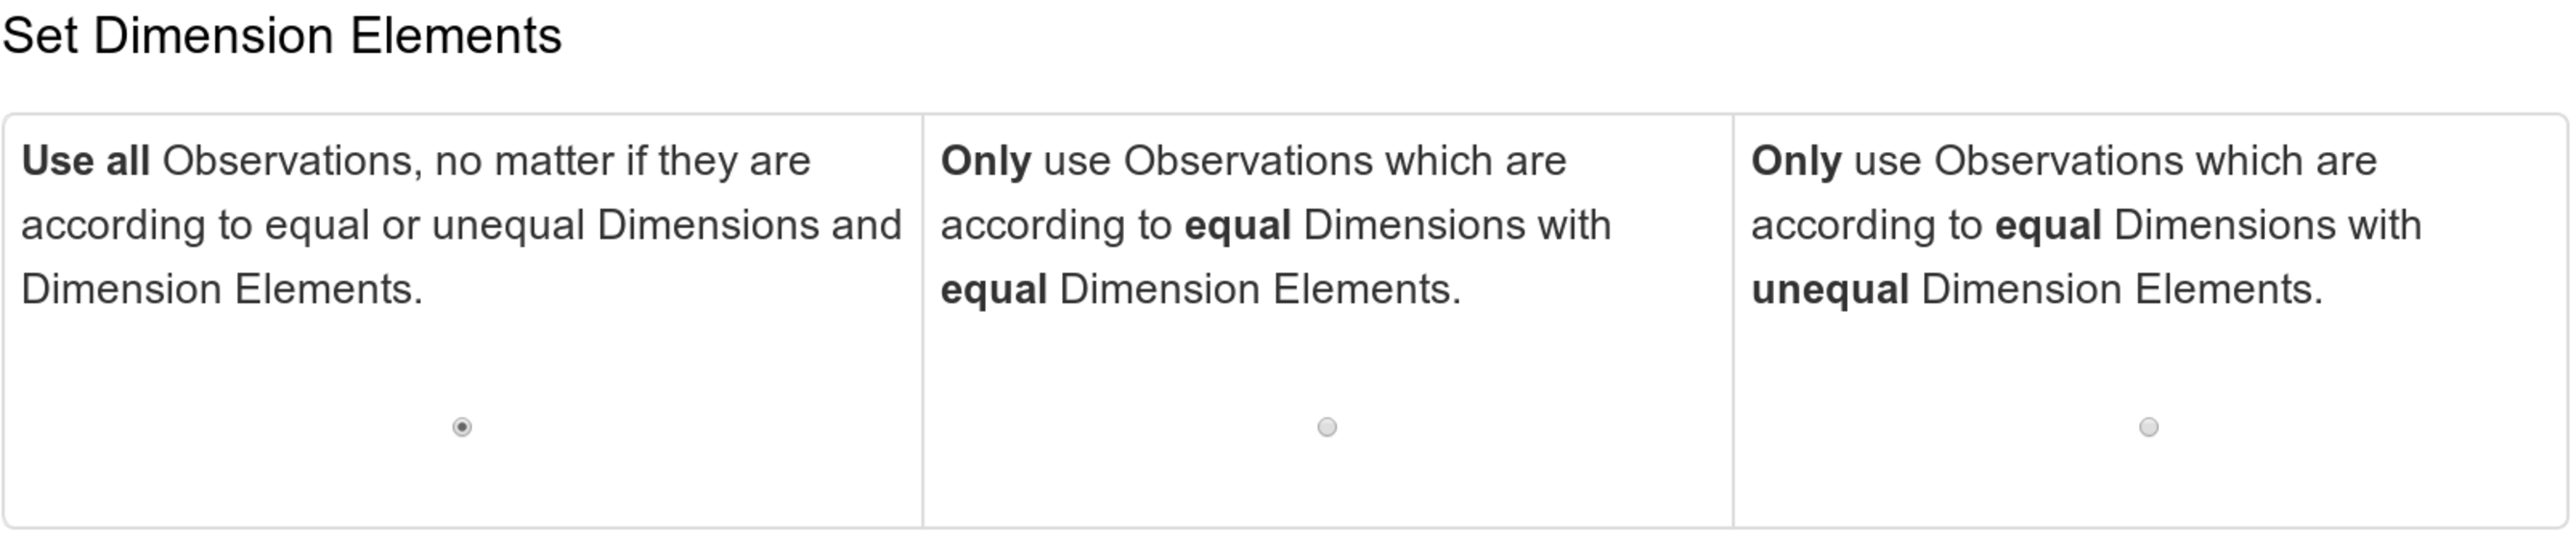
\includegraphics[width=15cm]{UserInterfaceMergeDatasets/DimensionelementSelectionUserInterface.pdf}
    \caption{Screenshot zur Auswahl der Dimensionselement-Art.}
    \label{fig:UserInterfaceMergeDatasets_DimensionelementSelectionUserInterface}
\end{figure}

Nach der Eingabemaske für die Normalisierung folgt eine Auswahl\com{Anforderung \\ F-350, S. \pageref{req:F350}} der Dimensionselemente, wobei hier nicht direkt einzelne Dimensionselemente ausgewählt werden, sondern der Benutzer nur bestimmen kann, ob er alle Beobachtungspunkte haben möchte oder nur die, welche jeweils gleichen bzw. ungleichen Dimensionselementen zugeordnet sind. Standardmäßig ist immer die Option für alle Beobachtungspunkte ausgewählt. 

\noindent
Wurde die Auswahl geändert, so stößt dies ebenfalls den Prozess der Zusammenführung erneut an. Ein Screenshot der Auswahl ist auf der Abbildung \ref{fig:UserInterfaceMergeDatasets_DimensionelementSelectionUserInterface} dargestellt.


%
% SSS
%
\subsubsection{Anzeige verfügbarer Visualisierungen}

Nach der Zusammenführung zweier Datensätze werden dazu passende\com{Anforderung \\ F-380, S. \pageref{req:F380}} Visualisierungen ermittelt und angezeigt. Ein Beispiel dafür, wie so etwas aussehen kann, ist auf der Abbildung \ref{fig:UserInterfaceMergeDatasets_PossibleVisualizations} zu sehen. \\

%
% Abbildung
%
\begin{figure}[h!]
    \centering
    \includegraphics[width=9cm]{UserInterfaceMergeDatasets/PossibleVisualizations.pdf}
    \caption{Beispielliste mit Visualisierungen für zusammengeführten Datensatz.}
    \label{fig:UserInterfaceMergeDatasets_PossibleVisualizations}
\end{figure}

\noindent
Jedes dieser Symbole ist mit einem Link\com{Anforderung \\ F-370, S. \pageref{req:F370}} hinterlegt und führt zu einer entsprechenden Darstellung im Visualisierungsbereich von CubeViz. Der Grund für dieses Vorgehen ist, dass man dieselben Daten aus verschiedenen \textit{Perspektiven} bzw. \textit{Blickwinkeln} betrachten kann; nicht zu verwechseln mit der Analogie Dimension zu Blickwinkel. Beim Kuchendiagramm (Pie-Chart) bekommt man einen guten Überblick über die Verhältnisse der Messwerte, im Liniendiagramm liegt der Fokus eher auf dem Verlauf von Werten. So bietet jeder Typ seine eigene \textit{Perspektive} auf die dargestellten Daten.

Dieser Ansatz ist bei CubeViz grundlegend und er bietet viel Potenzial. Von daher sollte er bei der Vergleichbarkeit von Datensätzen und ihren Werten ebenfalls zur Anwendung kommen. Aufgrund der Erweiterbarkeit der Visualisierungsschnittstelle sind weitere, teils sehr spezifische Visualisierungstypen denkbar.


%
% SSS
%
\subsubsection{Cluster-Bildung als alternativer Zugang zu den Messwerten \\}

%
% Abbildung
%
\begin{figure}[h!]
    \centering
    \includegraphics[width=15cm]{UserInterfaceMergeDatasets/ClusterUserInterface.pdf}
    \caption{Benutzeroberfläche zur Konfiguration von Clustern.}
    \label{fig:UserInterfaceMergeDatasets_ClusterUserInterface}
\end{figure}

Die optionale Anforderung \textit{F-430}\com{Anforderung \\ F-430, S. \pageref{req:F430}} beschreibt die Clusterbildung mit den Messwerten der ausgewählten Beobachtungspunkte. Diese Möglichkeit wurde als Bereicherung der existierenden Ansätze angesehen und deswegen implementiert. Es wird eine Eingabemaske bereitgestellt, welche sich direkt unter der Liste der verfügbaren Visualisierungen befindet. 

\newpage
\noindent
Abbildung \ref{fig:UserInterfaceMergeDatasets_ClusterUserInterface} zeigt einen Screenshot der Eingabemaske, welche bereits zwei Links für die Visualisierung enthält (siehe Liste unten). Jede Änderung in der maximalen Anzahl von Clustern bewirkt die Generierung eines künstlichen Datensatzes. Die generierten Datensätze können dann direkt nach einem Klick auf einen Link visualisiert werden. 

Ein kleiner Ausschnitt einer Clustervisualisierung ist auf der Abbildung \ref{fig:UserInterfaceMergeDatasets_ClusterVisualization} zu sehen. Die Idee hinter dem Clustering ist, dass man einen alternativen Zugang zu den Messwerten selbst bekommt und dem Benutzer soll so eine Vorstellung davon gegeben werden, welche Messwerte nahe beieinanderliegen und wie groß die Skala ist, auf der sie sich verteilen. \\

%
% Abbildung
%
\begin{figure}[h!]
    \centering
    \includegraphics[width=10cm]{RefreshedUserInterfaces/ClusterVisualization.pdf}
    \caption{Ausschnitt aus einer möglichen Clustervisualisierung.}
    \label{fig:UserInterfaceMergeDatasets_ClusterVisualization}
\end{figure}


%
% SSS
%
\subsubsection{Zusammengeführte Datensätze als Linked Data Mashup's}

Nachdem man zwei Datensätze erfolgreich zusammengeführt hat, kann man diese auf zwei Arten anderen Interessenten bereitstellen. Bei der einen kann man den Link dazu nutzen, den Visualisierungsbereich von CubeViz aufzurufen. Bei der anderen kann man direkt über HTTP die erzeugten RDF-Daten abfragen und weiterverarbeiten. Letztere Variante bietet die Möglichkeit, dass man sich den zusammengeführten Datensatz wieder als neuen Datensatz importieren und mit einem anderen zusammenführen kann.

Ein Merkmal der Linked Data Mashup's ist die Bereitstellung von Daten für eine bestimmte Domäne. 


\newpage
\noindent
Diese wird durch eine Ontologie definiert. Im Fall des zusammengeführten Datensatzes wäre die Ontologie zweigeteilt: Hauptsächlich würde er definiert durch das DataCube-Vokabular, aber zusätzlich durch das im Datensatz vorliegende Faktenwissen. 

Wenn es um die Quellen eines Linked Data Mashup's geht, dann muss man eigentlich auch den Benutzer mit einbeziehen. Er führt Datensätze zusammen, selektiert Daten und erstellt konkrete Sichten (Visualisierungen) auf sie. Das von ihm Erstellte kann wieder anderen zur Verfügung gestellt werden. Damit verhält er sich prinzipiell selbst wie ein Mashup und nimmt damit die Rolle einer Datenquelle ein. Dieses Gedankenspiel soll nicht weiter Gegenstand der weiteren Ausführungen sein, aber eine paar Ideen und alternative Interpretationen zu den bestehenden Fakten darlegen.




%
% SS
%
\subsection{Anpassungen der Legende}
\label{sec:chapterLegendAdaptions}

Nachdem die selbst entwickelte Benutzeroberfläche zur Zusammenführung von Datensätzen vorgestellt wurde, geht es nun um die Anpassung und Erweiterung der bestehenden Benutzeroberflächen von CubeViz, beginnend mit der Legende. 

Die Legende stellt in der aktuellen Version von CubeViz eine rudimentäre Übersicht über die Datenselektion und die eigentlichen Beobachtungspunkte dar. Hier eine Liste der Anforderungen, welche die erwähnten Schwachstellen betreffen:

\begin{itemize}
    \com{Anforderungen}
    \item Auf-\com{F-200, S. \pageref{req:F200}} und absteigende Sortierung nach Dimensionen und Messwert
    \item Anzeige\com{F-210, S. \pageref{req:F210}} aller Daten eines DataCube-Elements
    \item Anpassung\com{F-230, S. \pageref{req:F230}} einzelner Messwerte zur Veränderung der Visualisierung
\end{itemize}

\noindent
Zu dieser Liste kommen nun noch folgende Anforderungen hinzu:

\begin{itemize}
    \item Anzeige\com{F-220, S. \pageref{req:F220}} doppelter Beobachtungspunkte
    \item Originalwerte\com{F-240, S. \pageref{req:F240}} von Messwerten müssen permanent ersichtlich sein
\end{itemize}

\noindent
Doppelte Beobachtungspunkte können im Zuge der Zusammenführung von Datensätzen auftreten. Das geschieht, wenn sich beide Datensätze mindestens einen Beobachtungspunkt teilen. In diesem Fall gibt es, semantisch gesehen, keinen eindeutigen Messwert. 

\noindent
Der letzte Punkt der zweiten Liste fordert die permanente Anzeige der Originalwerte von Messwerten, falls sie verändert wurden. Dies erfolgt deshalb, damit die angepassten Originalwerte sichtbar gemacht werden, um Änderungen nachvollziehen zu können. Diese Anforderungen erhöhen zusammen den Grad an bereitgestellten Informationen und geben dem Benutzer mehr Möglichkeiten, sich diese zugänglich zu machen. Damit werden die Anwendungsfälle zur Exploration von statistischen Daten erheblich besser unterstützt.


%
% SSS
%
\subsubsection{Übersicht der Datenselektion}

%
% Abbildung
%
\begin{figure}[h!]
    \centering
    \includegraphics[width=12cm]{CubeViz/OldLegendDataSelection.pdf}
    \caption{Ausschnitt der Datenselektion der Legende von Version 0.9 für die Dimension \textit{Country}.}
    \label{fig:UserInterfaceMergeDatasets_OldLegendDataSelection}
\end{figure}

\noindent
Im Rahmen dieser Arbeit wurde der Legende eine größere Rolle zugedacht. Sie soll nun der Dreh- und Angelpunkt für weitreichende Informationen sowohl über die Datenselektion als auch über die Beobachtungspunkte werden.

Der Bereich der Datenselektion wurde komplett überarbeitet.\com{Anforderung \\ F-210, S. \pageref{req:F210} \\\\ Commits \\ 003fb0 \\ 4769fe} Er bietet nun mehr Informationen für die ausgewählten Elemente und erhielt eine Reihe von Verbesserungen. So werden nun die Schlüssel-Wert-Paare für die Datenstruktur Definition, den Datensatz, die Komponenten-Spezifikationen, den ausgewählten Messwert und, falls vorhanden, die Maßeinheit angezeigt. Informative Erklärungstexte zu den einzelnen Gruppen der DataCube-Elemente wurden ebenfalls hinzugefügt. Bisher gab es in diesem Bereich nur Informationen über die ausgewählten Dimensionen und ihrer Dimensionselemente; Informationen über die Datenstruktur Definition, den Datensatz, den Messwert und die Maßeinheit fehlten völlig.

Um\com{Anforderung \\ F-400, S. \pageref{req:F400}} die Navigation innerhalb der Legende zu verbessern, wurden HTML-Anker eingefügt. Das sind spezielle Links, welche nach einem Klick zu einem anderen Bereich springen ohne die Seite neu zu laden. Auf diese Weise kann man nun zwischen den Elementen der Datenselektion hin und her springen.

Im Zuge der Zusammenführung wurde die Anforderung \textit{F-10}\com{Anforderung \\ F-10, S. \pageref{req:F10}} erwähnt. Sie definiert, dass die Originaldaten immer ersichtlich sein müssen. Daher wird bei allen DataCube-Elementen ein zusätzlicher Bereich eingebunden, in dem die Schlüssel-Wert-Paare der ursprünglichen Elemente aufgelistet werden. \com{Commit \\ 2d63df} Auf diese Weise erlaubt man dem Benutzer, Vergleiche zwischen den künstlichen DataCube-Elementen und den Originalen zu ziehen. 

Die Abbildung \ref{fig:UserInterfaceMergeDatasets_ScreenshotExampleDim_new} zeigt einen Block der Benutzeroberfläche mit Informationen über eine Dimension. Im oberen Bereich findet man den Namen und einen Beschreibungstext, darunter dessen Titel, welcher ein Link auf die eigentliche Ressource ist. 

Im Vergleich zur Abbildung \ref{fig:UserInterfaceMergeDatasets_OldLegendDataSelection} hat man nun wesentlich mehr Informationen über das Element. Es wird nun weniger Platz für die Auflistung der Dimensionselemente benötigt, wobei es nun auf Knopfdruck kein Fenster mehr gibt, welche deren Schlüssel-Wert-Paare enthält. Mit dieser Änderung wurde der Fokus auf die eigentliche Dimension und ihre Komponenten-Spezifikation gelegt statt auf die einzelnen Dimensionselemente.


%
% Abbildung
%
\begin{figure}[h!]
    \centering
    \includegraphics[width=15cm]{RefreshedUserInterfaces/ScreenshotExampleDim_new.pdf}
    \caption{Block für eine Dimension nach der Überarbeitung.}
    \label{fig:UserInterfaceMergeDatasets_ScreenshotExampleDim_new}
\end{figure}

%
% SSS
%
\subsubsection{Liste der Beobachtungspunkte}

\noindent
Die Liste der Beobachtungspunkten wurde ebenfalls stark überarbeitet. Zum Vergleich sei auf die bisherige Benutzeroberfläche der Liste verwiesen, siehe dazu Abbildung \ref{fig:UserInterfaceMergeDatasets_OldLegend}. Auf ihr wird jeder Beobachtungspunkt von einer Box repräsentiert, welche den Titel, die genutzten Dimensionselemente, den Messwert und den Link auf die Quelle des Beobachtungspunktes enthält. \\

%
% Abbildung
%
\begin{figure}[h!]
    \centering
    \includegraphics[width=15cm]{CubeViz/OldLegend.pdf}
    \caption{Ausschnitt der Benutzeroberfläche des Bereichs der Beobachtungspunkte der Legende von CubeViz in Version 0.9.}
    \label{fig:UserInterfaceMergeDatasets_OldLegend}
\end{figure}

Die Liste wurde in eine Tabelle umgewandelt, welche mehr Informationen und Funktionen für den Betrachter zur Verfügung stellt. Die Spalten der Tabelle sind einerseits die ausgewählten Dimensionen und andererseits der ausgewählte Messwert. Es wurde dafür die Funktion \verb|displayRetrievedObservations()|\com{Commit \\ 84004a} aus der Datei \verb|View/| \verb|IndexAction/Legend.ts| angepasst. Standardmäßig werden die Beobachtungspunkte nun nach dem Messwert aufsteigend sortiert.

\newpage
\noindent
Durch die Umstellung der Liste zu einer Tabelle konnte die Anforderung \textit{F-200}\com{Anforderung \\ F-200, S. \pageref{req:F200}} durch folgende Anpassungen der gerade genannten Datei realisiert werden:

\begin{itemize}
    \item Funktionen \verb|sortDimensionsAscOrDesc()| und \verb|sortMeasureValueAscOrDesc()| hinzugefügt
    \item Funktionen \verb|sortByTitle()| und \verb|sortByValue| gelöscht
\end{itemize}

\noindent
Nach dieser Änderung gibt es eine Funktion für die Sortierung der Beobachtungspunkte nach den Dimensionselementen und eine für die Sortierung nach dem Messwert. Die Art der Sortierung, also auf- oder absteigend, wird über einen Parameter gesteuert. Die Abbildung \ref{fig:RefreshedUserInterfaces_NewObservationList} beinhaltet den Kopf und zwei Elemente der neugestalteten Liste. In jeder Spalte findet man ein paar Symbole, darunter \includegraphics[width=0.38cm]{RefreshedUserInterfaces/sortUp.pdf} und \includegraphics[width=0.38cm]{RefreshedUserInterfaces/sortDown.pdf}. \com{Anforderungen \\ F-70, S. \pageref{req:F70} \\ F-220, S. \pageref{req:F220}}Nach einem Klick auf eines davon wird die Liste anhand der enthaltenen Elemente der zugehörigen Spalte auf- bzw. absteigend sortiert. Während der Zusammenführung kann es vorkommen, dass beide Datensätze jeweils gleiche Beobachtungspunkte besitzen. In diesem Fall erstellt CubeViz einen künstlichen Beobachtungspunkt im zusammengeführten Datensatz, welcher Referenzen auf die beiden anderen enthält. Weiterhin bedeutet das später für CubeViz, dass es für diesen Beobachtungspunkt keinen eindeutigen Messwert gibt, was durch eine entsprechende Meldung in der Legende dargestellt wird.\\

%
% Abbildung
%
\begin{figure}[h!]
    \centering
    \includegraphics[width=15.3cm]{RefreshedUserInterfaces/NewObservationList.pdf}
    \caption{Kopfbereich der neugestalteten Liste der Beobachtungspunkte in der Legende.}
    \label{fig:RefreshedUserInterfaces_NewObservationList}
\end{figure}

\noindent
Zudem wird eine ausklappbare Liste der Schlüssel-Wert-Paare beider ausgehender Beobachtungspunkte eingeblendet. Die Abbildung \ref{fig:RefreshedUserInterfaces_Screenshot_DoubledObservationsInLegend} enthält die Anzeige eines künstlichen Beobachtungspunktes, welcher aufgrund zwei gleicher Beobachtungspunkte erstellt wurde.

Die Anforderung \textit{F-230}\com{Anforderung \\ F-230, S. \pageref{req:F230}} beschreibt eine hilfreiche Funktion bei der Exploration von statistischen Daten. Dabei geht es um die zeitweilige Veränderung einzelner Messwerte, um damit unmittelbar deren Visualisierung anzupassen. Durch die entsprechende Anpassung der Dateien \verb|View/IndexAction/Legend.ts|, \verb|Model/HighCharts/Charts.ts| und\com{Commit \\ b5088a} \verb|Model/D3js/Circle| \verb|Packing.ts| ist es nun möglich, bestehende Messwerte live anzupassen, wie in Anforderung \textit{F-230} gefordert.

%
% Abbildung
%
\begin{figure}[h!]
    \centering
    \includegraphics[width=15.3cm]{RefreshedUserInterfaces/Screenshot_DoubledObservationsInLegend.pdf}
    \caption{Beispielhafte Anzeige eines künstlichen Beobachtungspunktes, der aus zwei gleichen hervorgegangen ist.}
    \label{fig:RefreshedUserInterfaces_Screenshot_DoubledObservationsInLegend}
\end{figure}

\newpage
\noindent
Anforderung \textit{F-240}\com{Anforderung \\ F-240, S. \pageref{req:F240}} spielt im Zusammenhang mit der Änderung von bestehenden Messwerten eine wichtige Rolle. Sie fordert, dass die Originalwerte weiterhin ersichtlich sein müssen. Erkennt CubeViz einen geänderten Messwert, so wird neben diesem der Originalwert angezeigt. \\

%
% Abbildung
%
\begin{figure}[h!]
    \centering
    \includegraphics[width=15cm]{RefreshedUserInterfaces/LineOfObservationListForOriginalValue.pdf}
    \caption{Beispiel für Darstellung des Originalwertes zu einem geänderten Messwert.}
    \label{fig:RefreshedUserInterfaces_LineOfObservationListForOriginalValue}
\end{figure}

\noindent
Geänderte Messwerte sind ermittelbar, weil diese in einer neuen CubeViz-Eigenschaft des JSON-Objektes namens \verb|__cv_temporaryNewValue| abgelegt werden. CubeViz prüft, ob diese Eigenschaft definiert wurde. Wenn ja, dann besitzt der zugehörige Beobachtungspunkt einen Originalwert und einen vom Benutzer angepassten Wert. Die Abbildungen \ref{fig:RefreshedUserInterfaces_LineOfObservationListForValueAdaption} und   \ref{fig:RefreshedUserInterfaces_LineOfObservationListForOriginalValue} stellen Screenshots dazu bereit. \\

%
% Abbildung
%
\begin{figure}[h!]
    \centering
    \includegraphics[width=15cm]{RefreshedUserInterfaces/LineOfObservationListForValueAdaption.pdf}
    \caption{Beispiel für Eingabemaske zur Anpassung eines Messwertes.}
    \label{fig:RefreshedUserInterfaces_LineOfObservationListForValueAdaption}
\end{figure}

\noindent
Die optionale Anforderung \textit{F-410}\com{Anforderung \\ F-410, S. \pageref{req:F410}} hat sich als nützlich erwiesen und wurde daher implementiert. Nun sieht man, wie viele Dimensionselemente eine Dimension insgesamt besitzt und wie viele überhaupt in den angezeigten Beobachtungspunkten benutzt wurden. 

\newpage
\noindent
Dafür wurde die Funktion\com{Commit \\c08a21} \verb|getUsedDimensionElementUris()| zur Datei \verb|Model/DataCube/| \verb|Observation.ts| hinzugefügt. Zur Illustration sei auf die Abbildung \ref{fig:RefreshedUserInterfaces_NewObservationList} verwiesen.


%
% SS
%
\subsection{Anpassungen im Visualisierungsbereich}
\label{sec:chapterVisualizationAdaptions}

Eine Reihe von Erweiterungen und Veränderungen wurde im Visualisierungsbereich von CubeViz durchgeführt. Für den Visualisierungsbereich sind alle Dateien verantwortlich, welche unmittelbar an der Erstellung einer Visualisierung beteiligt sind. Zuerst werden eine Reihe von Anpassungen und Erweiterungen kurz und knapp dargelegt, danach folgt die Einführung einer neuen Visualisierungsbibliothek und der damit verbundenen Änderungen im Code von CubeViz.

%
% SSS
%
\subsubsection{Allgemeine Anpassungen und Erweiterungen}

Die Datei\com{Commit \\ 3ecf81 \\ 7635c0} \verb|Model/CubeViz/Visualization/HighCharts/Chart.ts| wurde so überarbeitet, dass für jeden der Fälle, der bei der Visualisierung eintreten kann, eine eigene Funktion genutzt wird. Folgende Fälle sind hier gemeint: Datensatz hat zwei multiple Dimensionen, eine multiple Dimension oder eine Dimension mit einem Element. Statt alles in einer Funktion abzuarbeiten, wurde dies nun auf drei verteilt und das resultiert in einem klareren Vorgehen bei der Abarbeitung.

Die Reaktivierung\com{Commit \\ c7ace6} der auskommentierten Funktion \verb|sortAxis()| aus der Datei \verb|Model/Data| \verb|Cube/Observation.ts| bewirkt nun eine aufsteigende Sortierung der Labels von Dimen-sionselementen auf der X-Achse. Der Grund dafür war, dass auf diese Weise immerhin gleich benannte Dimensionselemente nebeneinander gestellt werden, auch wenn sie ungleich sind. Dies soll das Verständnis und die Übersicht über die Daten verbessern.

Die Funktion \verb|setTooltip()|\com{Commit \\f8e353} wurde zur Visualisierung hinzugefügt, um für jeden dargestellten Beobachtungspunkt zusätzliche Informationen anzuzeigen. Ergänzend dazu wurde die JavaScript-Bibliothek \textit{underscorejs.string}\footnote{\url{http://epeli.github.io/underscore.string}} genutzt, um ein einheitliches Erscheinungsbild der Messwerte zu gewährleisten.

%
% SSS
%
\subsubsection{Neue Visualisierungsbibliothek: D3js}

Es wurde eine neue Visualisierungsbibliothek namens D3js\footnote{\url{http://d3js.org}} hinzugefügt. Im Rahmen dieser Arbeit wurde aufgrund der begrenzten Zeit jedoch nur die Visualisierung namens \textit{Circle Packing} in CubeViz implementiert. Sie ist flexibel und bietet einerseits die Möglichkeit, Cluster anzuzeigen und andererseits, mit Datensätzen umzugehen, die mehr als zwei multiple Dimensionen besitzen. \com{Commits \\ 335557} Die Datei \verb|View/IndexAction/Visualization.ts| wurde so angepasst, dass eine getrennte Initialisierung von HighCharts- und D3js-Visualisierungen möglich wurde. Zudem wurde die Funktion \verb|getDefaultChartConfig()| hinzugefügt,\com{3742ab} um basierend auf der Anzahl der multiplen Dimensionen, standardmäßig eine valide Chart-Konfiguration laden zu können.


%
% SS
%
\subsection{Sonstige Änderungen}
\label{sec:chapterMiscAdaptions}

An dieser Stelle werden Änderungen an den Dateien aufgeführt, die bereichsübergreifend genutzt werden. Der Fokus liegt in diesem Kapitel auf den wesentlichen Änderungen.

CubeViz benutzt die Symbole des \textit{semicon}-Projekts\footnote{\url{https://github.com/k00ni/semicon}}. Dieses enthält speziell für die einzelnen Bereiche des Semantic Web zugeschnittene Symbole. Einige davon wurden in der neu entwickelten Oberfläche zur Zusammenführung von Datensätzen genutzt. Da weitere Symbole nötig wurden, hat sie der Autor neu erstellt und danach dem semicon-Projekt zur weiteren Nutzung zur Verfügung gestellt. Darunter befanden sich Symbole für die Dimensionselemente, die Datenstruktur Definition sowie den Datensatz (siehe Abbildung \ref{fig:semicon_addedIcons}). \\

%
% Abbildung
%
\begin{figure}[h!]
    \centering
    \includegraphics[width=0.6cm]{semicon/dataset3.pdf} \quad \ 
    \includegraphics[width=0.8cm]{semicon/dataStructureDefinition.pdf} \quad \ 
    \includegraphics[width=0.8cm]{semicon/equalDimensionElements.pdf} \quad \ 
    \includegraphics[width=0.8cm]{semicon/equalDimensionElements2.pdf} \quad
    \includegraphics[width=0.8cm]{semicon/equalDimensionElements3.pdf} \quad
    \includegraphics[width=1cm]{semicon/equalDimensionElements4.pdf} \quad
    \includegraphics[width=0.8cm]{semicon/equalDimensionElements5.pdf} \quad
    \includegraphics[width=0.8cm]{semicon/unequalDimensionElements.pdf} \quad
    \includegraphics[width=0.8cm]{semicon/unequalDimensionElements2.pdf} \quad
    \includegraphics[width=0.8cm]{semicon/unequalDimensionElements3.pdf} 
    \caption{Liste aller neu hinzugefügten Icons zum semicon-Projekt.}
    \label{fig:semicon_addedIcons}
\end{figure}

Es wurde die Funktion \verb|parseValue()| zur Datei \verb|Model/DataCube/Observation.ts| hinzugefügt. Sie wird von nun an in verschiedenen Teilen des CubeViz verwendet, um die sichere Behandlung des Messwertes zu gewährleisten. Der Messwert kann laut Spezifikation entweder eine Zahl oder auch eine Zeichenkette sein. Man vertritt in CubeViz eine liberale Position, wie Messwerte gestaltet sein müssen, so können sie beispielsweise Leerzeichen enthalten. Bisher wurde an verschiedenen Stellen immer der gleiche Code zur Behandlung von Messwerten eingesetzt, doch nun nutzen alle diese Stellen die neue Funktion.

Im Verlauf der Implementierung wurde es nötig, die bestehenden JSON-Objekte um weitere CubeViz-eigene Eigenschaften zu erweitern. Dazu eine Liste: 

\begin{itemize}
    \item \verb|__cv_temporaryNewValue|: Speichert den vom Benutzer eingetragenen Wert für einen Beobachtungspunkt (betrifft Anforderung \textit{F-230})
    
    \item \verb|__cv_sourceDataSet|, \verb|__cv_componentSpecification| und \verb|__cv_Observation| speichern jeweils die ursprünglich verwendeten Originaldaten (Relevant im Rahmen der Zusammenführung von Datensätzen)
    
    \item \verb|__cv_active| legt fest, ob ein Element genutzt werden soll (true) oder nicht (false). Wird für Beobachtungspunkte genutzt, welche auf diese Weise sichtbar oder unsichtbar werden.
    
    \item \verb|__cv_double| speichert den Zwilling eines Elements.
\end{itemize}

Die Exportfunktion von CubeViz wurde so angepasst,\com{Anforderung \\ F-390, S. \pageref{req:F390} \\ \\ Commit \\ 58f2e7} dass sie es ermöglicht, die RDF-Daten zusammengeführter Datensätze bereitzustellen (\emph{F-390}). Es wurde die Funktion \verb|save()| der Datei \verb|Model/CubeViz/ConfigurationLink.ts| aufgeteilt in \verb|saveData()| und \verb|saveUI()|. 

\newpage
\noindent
Erstere übernimmt ausschließlich die Speicherung von DataCube-Daten, letztere nur noch die für die Visualisierung relevanten Informationen. Diese Aufteilung wurde deshalb nötig, damit man nun je eine Funktion für eine Aufgabe hat. Weiterhin wurde der Hash anfänglich innerhalb der Funktion \verb|save()| basierend auf dem übergebenen Datenobjekt generiert. Dies wurde abgeändert und nun wird derselbe Hash sowohl für die URI's genutzt als auch zur Speicherung der Daten. Somit sind Daten direkt mit dem Hash verbunden und sauber dereferenzierbar. Daten werden von nun an direkt abgespeichert, die Generierung des Hashes wurde vom Server auf den Client verlagert.

%
%
%
% ------------------------------------------------------------------------
\newpage
\section{Evaluation und Kritik}
\label{sec:chapterEvaluation}

Im Rahmen dieses Kapitels werden die getätigten Änderungen aus dem Implementierungskapitel aufgelistet und selbstkritisch diskutiert. Grundlage für dieses Vorgehen sind die eingangs genannten Anwendungsfälle:

\begin{itemize}
    \item \nameref{sec:chapterUC1}
    \item \nameref{sec:chapterUC2}
    \item \nameref{sec:chapterUC3}
\end{itemize}

\noindent
Im Verlauf der Arbeit wurde die bisherige Umsetzung und Unterstützung dieser Fälle in CubeViz dargelegt und aufgezeigt, wo es Schwachstellen gibt. Diese Schwachstellen wurden dann beschrieben und eine Reihe von Maßnahmen erarbeitet um sie zu beheben. Bereits im Verlauf des Implementierungskapitels wurde eine teils vergleichende Betrachtung zwischen der vorherigen und der aktuellen Funktionalität durchgeführt. Diese Betrachtungen werden nun konkretisiert und die folgenden Unterkapitel evaluieren das Endergebnis dieser Anpassungen unter den Gesichtspunkten der Benutzbarkeit und Performance. Abschließend wird noch einmal auf CubeViz als Linked Data Mashup eingegangen und in welcher Form die Änderungen im Rahmen dieser Arbeit dies verändert hat.


%
% SS
%
\subsection{Aspekt der Benutzbarkeit}
\label{sec:chapterEvaluationAspectUsability}

Die erste Evaluation erfolgt unter dem Gesichtspunkt der Benutzbarkeit. Da dies ein recht ungenauer Begriff ist, soll er durch folgende Kriterien konkretisiert werden.

\begin{itemize}

    \item Anzahl der Schritte um eine Aufgabe zu erledigen
    
    \item Den Umfang bereitgestellter Informationen über DataCube-Elemente
    
    \item Anzahl der Möglichkeiten bei der Exploration von Daten

\end{itemize}

%
%
%
\subsubsection{Kriterium: Anzahl der Schritte}

Das Kriterium beschreibt, wie viele Schritte und damit auch, wie lange jemand benötigt, um eine konkrete Aufgabe zu erledigen. Der Zeitfaktor spielt bei der Benutzbarkeit einer Software eine große Rolle und dient damit letztendlich auch dem effektiven Arbeiten. Im Folgenden werden die einzelnen Schritte für die Durchführung jedes Falls aufgeführt. Danach wird erläutert, wo es Einsparungen gab und wie sich dies auf die Benutzbarkeit ausgewirkt hat.

\paragraph{\nameref{sec:chapterUC1}} Hierbei wurden keine Anpassungen für dieses Kriterium durchgeführt und daher auch keine Verbesserungen erzielt. \\

\paragraph{\nameref{sec:chapterUC2}} 


Bei diesem Fall wurden viele Anpassungen und Erweiterungen durchgeführt. Zur Übersicht der Abläufe in der vorherigen und aktuellen Version sei auf folgende Abbildung \ref{fig:Evaluation_UseCase2_OldNew} verwiesen. \\


%
% Abbildung
%
\begin{figure}[h!]
    \centering
    \includegraphics[width=15cm]{Evaluation/UseCase2_OldNew.pdf}
    \caption{Ablaufplan des zweiten Anwendungsfalls, vor den Anpassungen und danach.}
    \label{fig:Evaluation_UseCase2_OldNew}
\end{figure}

\noindent
Auf dieser Abbildung ist auf der linken Seite der Ablaufplan der vorherigen Version illustriert, die rechte Seite zeigt den der aktuellen Version. In der vorherigen Version\com{Vorherige Version} war es nötig, die Daten in eine eigene CubeViz Instanz zu importieren, wollte man gewisse Messwerte anpassen. Dies erforderte den Export der Datenselektion auf der Quellinstanz, was nur möglich war, falls der Autor der Quellinstanz die Exportfunktionalität aktiviert hatte. Ebenso war die händische Anpassung der Werte in den RDF-Tripeln und der Import in eine eigene CubeViz-Instanz nötig. Erst danach konnte man dem Autor der Quellinstanz eine andere Sicht auf seine Daten mit angepassten Werten zeigen. Dabei gab es eine Reihe von Problemen. So waren die Originalwerte nicht mehr erkennbar und die Datenselektion musste erst wieder manuell hergestellt werden. Zudem müsste der Autor die gleichen Schritte auf seiner Instanz durchführen, um dem anderen seine geänderten Werte zu zeigen.

In der aktuellen Version\com{Aktuelle\\ Version} entfallen einige dieser Schritte und die damit verbundenen Probleme. Es ist nun möglich, innerhalb der Quellinstanz des Autors direkt die Werte anzupassen und damit eigene Sichten mit Visualisierungen zu generieren. Man verlässt die Quellinstanz nicht mehr, für Export, Anpassung der Werte und Import, und man braucht ebenfalls keine eigene CubeViz-Instanz. Weiterhin bleiben die Originalwerte erkennbar und die Wiederherstellung der Datenselektion in der eigenen CubeViz-Instanz entfällt auch.

\paragraph{\nameref{sec:chapterUC3}} Im Rahmen der Implementierung wurde eine eigene Benutzeroberfläche nebst Funktionen implementiert, um den alten Ablauf in neuer Form abzubilden. Die vorherige Version\com{Vorherige Version} machte es nötig, dass man zwei getrennte Browser-Tabs oder -Instanzen mit CubeViz benutzen musste. In beiden muss man jeweils die Datenselektion für die beiden zu vergleichenden Datensätze durchführen und dann die Werte in der Legende finden, die man vergleichen will. Aus praktischer Sicht müsste man dann die beiden CubeViz-Instanzen nebeneinander stellen oder ständig zwischen ihnen hin und her springen. 

\newpage
\noindent
Folgende Probleme ergeben sich hier:

\begin{itemize}
    \item Zeitaufwand für die genaue Datenselektion
    \item Zeitaufwand für Einrichtung der CubeViz-Instanzen zur späteren optischen Betrachtung
\end{itemize}

\noindent 
Aber es gibt noch eine Reihe weiterer inhaltliche Probleme:

\begin{itemize}
    \item Keine gemeinsame Visualisierung der Werte möglich
    \item Keine Normalisierung der Werte möglich (da bisher noch nicht implementiert)
    \item Keine Gegenüberstellung der Werte 
\end{itemize}

\noindent
Um diese Probleme händisch zu lösen, benötigt man einerseits fortgeschrittene Kenntnisse in RDF und dem DataCube-Vokabular und andererseits ein gutes Verständnis der vorliegenden statistischen Daten. Ist das gegeben, so könnte jedermann die genannten drei Probleme beheben, indem er die Datensätze entsprechend anpasst oder gleich selbst zusammenführt. Er würde dafür aber einen erheblichen Zeitaufwand benötigen, je nach Umfang der Datensätze und Werkzeuge. Das Kriterium der benötigten Schritte greift hier ebenso, da zusätzlicher Zeitaufwand weitere Arbeitsschritte bedeutet. 

Trotzdem bleibt zu erwähnen, dass die getrennte bzw. händische Datenselektion eine viel höhere Genauigkeit\com{Höhere Genauigkeit} zulässt als die neue Benutzeroberfläche. Daher ist die alte Form eher für Experten geeignet, die direkt auf RDF-Ebene mit den Daten arbeiten und CubeViz lediglich zur Visualisierung nutzen wollen. Trotz Einführung der neuen Benutzeroberfläche, ist dies auch in der neuen Version weiterhin möglich.

In der aktuellen Version\com{Aktuelle \\ Version} wurden die obigen Probleme weitestgehend gelöst. Man muss nun nicht mehr CubeViz verlassen, um zwei Datensätze zusammenzuführen. Diese können nun direkt ausgewählt werden und man erhält eine Gegenüberstellung von statistischen Informationen über die Datensätze und enthaltene Messwerte. Durch die darauffolgende Zusammenführung erfolgt die Generierung eines eigenständigen Datensatzes, welcher die Beobachtungspunkte der beiden Ausgangsdatensätze enthält. Damit kann nun eine gemeinsame Visualisierung der Werte stattfinden. Vor der Zusammenführung kann eine Normalisierung über eine frei definierbare Formel durchgeführt werden, um die Skalen der Messwerte einander anzugleichen. Damit entfällt auch die händische Anpassung der Werte.

Wie bereits erwähnt, bietet die vorherige Version eine höhere Genauigkeit bei der Datenselektion. Sie ist zwar auch in der aktuellen Version noch möglich, aber die neue Oberfläche wurde mit dem Fokus auf solche Benutzer entwickelt, welche keine guten Kenntnisse im Umgang mit RDF-Daten besitzen. Auf diese Weise ergänzen sich die beiden Versionen.

%
%
%
\subsubsection{Kriterium: Umfang bereitgestellter Informationen}

Die bereitgestellten Informationen betreffen die DataCube-Elemente und deren Schlüs-sel-Wert-Paare. Mit diesem Kriterium ist gemeint, in welcher Form und Tiefe Informationen zu Data-Cube Elementen dargestellt werden.  

\paragraph{\nameref{sec:chapterUC1}} Bei der Exploration der Daten eines Datensatzes ist es besonders wichtig, dass die verfügbaren Information in adäquater Weise dargestellt werden, denn der Betrachter möchte sich ein Bild darüber machen, was der Datensatz an relevanten Dingen bereithält.

In der vorherigen Version\com{Vorherige Version} war die Legende der einzige Ort, um sich über die Beobachtungspunkte selbst zu informieren. Die Meta-Daten konnte man über das linke Seitenmenü abfragen, aber auch eingeschränkt in der Legende. Beide stellten jedoch nur selektiv Daten bereit, wie den Titel oder die Beschreibung. Wurden vom Autor der Daten zusätzliche Schlüssel-Wert-Paare an DataCube-Elemente angehängt, so konnte man sie oft nicht einsehen.

In der aktuellen Version\com{Aktuelle \\ Version} hat sich das grundlegend verändert. Die Legende wurde so angepasst, dass sie sowohl alle Schlüssel-Wert-Paare der Meta-Daten enthält, als auch eine verbesserte Liste der Beobachtungspunkte. Diese wurde neu strukturiert und enthält ebenfalls zusätzliche Informationen. Basiert ein Beobachtungspunkt beispielsweise auf einem anderen, so werden die Schlüssel-Wert-Paare des Original-Beobachtungspunktes ebenfalls eingeblendet. Dem Benutzer stehen nun also mehr Informationen zur Verfügung.


\paragraph{\nameref{sec:chapterUC2}} Für die kollaborative Zusammenarbeit ist eine ausreichende Menge an Informationen ebenfalls wichtig, um eine gemeinsame Datenbasis zu gewährleisten. Die Frage, was als ausreichend anzusehen ist, wurde im Rahmen dieser Arbeit nicht beantwortet. Jedoch wurden einige Kriterien vorgestellt, welche besondere positive Einflüsse auf die Kollaboration haben können. Dazu gehört die Anzeige von Originalwerten, falls diese verändert wurden, aber auch die Hervorhebung der im Zusammenhang mit der Zusammenführung von Datensätzen möglicherweise auftretenden doppelten Beobachtungspunkte. Es wird postuliert, dass ein höherer Grad an verfügbaren Informationen positiv zur Kollaboration beiträgt.  


\paragraph{\nameref{sec:chapterUC3}} Bei der Entwicklung der Oberfläche zur Zusammenführung von Datensätzen wurde ebenfalls darauf geachtet, soviele Informationen wie nötig in entsprechender Form darzustellen. So gibt es statistische Informationen über die Datensätze selbst und deren Messwerte. Der Bereich zur Generierung von Clustern soll dem Benutzer einen alternativen Überblick der Messwerte eines Datensatzes bereitstellen. 

Die Benutzeroberfläche ist noch sehr ausbaufähig. So lässt sie eine vollständige Datenselektion bei der Zusammenführung vermissen. Dies übernimmt nun erst einmal das linke Seitenmenü, aber erst nach der Zusammenführung. 

\newpage
\noindent
Weiterhin wäre eine breite Übersicht der enthaltenen Daten, und wie sie zusammenhängen, wünschenswert. Dazu würde z.B. auch eine Übersicht doppelter Beobachtungspunkte zählen.


%
%
%
\subsubsection{Kriterium: Möglichkeiten der Exploration}

Mit diesem Kriterium ist gemeint, in welcher Form CubeViz den Benutzer bei der Exploration der Daten unterstützt und welche (neuen) Werkzeuge es für welche Aufgaben bereitstellt.


\paragraph{\nameref{sec:chapterUC1} und \nameref{sec:chapterUC2}} Die Erweiterung der Legende um eine auf- und absteigende Sortierung der Dimensionselemente sowie den Messwert war ein wichtiger Schritt im Umgang mit den Beobachtungspunkten. Die vorherige Sortierung nach Titel und Messwert des Beobachtungspunktes führt nicht weit genug, denn nicht alle Beobachtungspunkte besitzen einen Titel. Eine Sortierung nach den Dimensionselementen war naheliegend, weil die Beobachtungspunkte über die Dimension identifiziert werden. Zuletzt besitzt der Betrachter durch die Veränderbarkeit einzelner Messwerte die Möglichkeit, die Visualisierung und damit seine Sicht auf die Daten anzupassen. Man könnte darüber nachdenken,\com{Anforderung \\ F-420, S. \pageref{req:F420}} eine Art Verlauf anzulegen, der speichert, wer zu welchem Zeitpunkt welche Werte geändert hat.

Diese Möglichkeiten kommen einem sowohl bei der alleinigen als auch bei der kollaborativen Exploration von Datensätzen zugute. Man sieht nun streckenweise mehr Informationen über die DataCube-Elemente und besitzt eine Reihe neuer Werkzeuge für die Exploration.


\paragraph{\nameref{sec:chapterUC3}} In der neugeschaffenen Oberfläche für die Zusammenführung wurden nicht sehr viele Möglichkeiten zur tiefer gehenden Exploration geschaffen. Man erhält eher allgemeine statistische Informationen, wie beispielsweise über die Anzahl der jeweiligen Elementgruppen. Der Betrachter kann erst nach der Zusammenführung die Meta-Daten und Beobachtungspunkte explorieren. 

Jedoch ist es möglich, über die im unteren Teil angebaute Eingabemaske die Messwerte des zusammengeführten Datensatzes zu clustern. Damit wird dem Benutzer eine alternative Exploration angeboten, bei der die Messwerte im Mittelpunkt stehen. In der vorgeschlagenen Kreis-Visualisierung kann man die verschiedenen Gruppen anschauen. Jedem Cluster-Element ist ebenfalls der ursprüngliche Beobachtungspunkt zugeordnet, den man sich in der Legende anschauen kann.

%
% SS
%
\subsection{Aspekt der Performance}
\label{sec:chapterEvaluationAspectPerformance}

In diesem Unterkapitel wird der Aspekt der Performance unter funktionalen Gesichtspunkten betrachtet. Es ist anzumerken, dass die Zielsetzung der Entwicklung nicht war, die Performance zu verbessern. Der Fokus lag auf der Steigerung der Benutzerfreundlichkeit. Trotzdem wurde während der Implementierung immer wieder darauf geachtet, die Funktionen so ressourcenschonend wie möglich zu realisieren.

%
%
%
\subsubsection{Vorstellung der Testszenarien und -systeme}

Es werden verschiedene Szenarien mit dem geänderten CubeViz auf zwei verschiedenen Systemen gemessen. Die Softwareumgebung auf diesen Systemen ist jeweils gleich, sie unterscheiden sich nur in ihrer Hardware. (siehe dazu Tabelle \ref{tab:evaluationTestEnvironment}) \\

\begin{table}[htbp]
\small
\begin{tabularx}{400pt}{p{1.5cm} p{4.7cm} p{2cm} p{3.9cm}}
    \textbf{ID} &
    \textbf{Prozessor} &
    \textbf{RAM} &
    \textbf{Festplatte}
\\
\toprule 
\\[0.1cm]
    Desktop-Computer & \mbox{Intel i5-3300}, \mbox{4 Kerne mit jeweils 3 GHz} & \mbox{8 GB} \mbox{DDR3-RAM} & 1 TB mit 7200 RPM \mbox{(Rotations per Minute)} \\[0.4cm]
    
\toprule    
\\[0.1cm] 
    
    Laptop & \mbox{Intel Pentium P6200}, \mbox{2 Kerne mit jeweils 2,13 GHz} & \mbox{2 GB} \mbox{DDR2-RAM} & 250 GB mit 5400 RPM (Rotations per Minute) \\[0.2cm]

\bottomrule

\end{tabularx}
\caption{Hardware der zwei Testsysteme.}
\label{tab:evaluationTestEnvironment}
\end{table}


\noindent
Die Hardware des Desktop-Computers entspricht einem Computersystem mit gehobener Ausstattung. Im Vergleich dazu ist der Laptop im unteren Leistungsbereich anzusiedeln. Die\com{Software-umgebung} Softwareumgebung sieht bei beiden folgendermaßen aus:

\begin{itemize}
    \item Betriebssystem: Ubuntu 12.04.2 LTS, 64 Bit
    \item Webserver: Apache HTTP Server 2.2.22
    \item Datenbank: Openlink Virtuoso 6.1.4
    \item Browser: Chromium 25
    \item PHP-Laufzeitumgebung: 5.3.10 mit Suhosin-Patch
    \item OntoWiki in Version 0.9.10 mit der Standard-Theme (silverblue)
\end{itemize}

\noindent
Wie der Liste zu entnehmen ist, wird auf beiden Systemen die Datenbank lokal ausgeführt. Sie bildet zusammen mit dem Apache Webserver die Testumgebung. Über den Browser wird die lokale CubeViz Installation aufgerufen und getestet. \\

\begin{table}[htbp]
\small
\begin{tabularx}{400pt}{>{\centering}p{2cm} >{\centering}p{4cm} >{\centering}p{4cm} p{3.4cm}}
    \textbf{ID} &
    \textbf{Anzahl Datensätze} &
    \textbf{Anzahl Dimensionen} &
    \textbf{Anzahl Tripel}
\\
\toprule 

    1 & 1 & 2 & \hfil 208 \hfil \\[0.4cm]
    
    2 & 1 & 2 & \hfil 213 \hfil \\

\toprule    
\\
    
    3 & 151 & 2 & \hfil 359.323 \hfil \\[0.2cm]
    
\bottomrule

\end{tabularx}
\caption{Allgemeine Statistik der Test-DataCube's.}
\label{tab:evaluationOverviewTestDataCubes}
\end{table}


\noindent
Es werden nun die verwendeten Datensätze vorgestellt. In der Tabelle \ref{tab:evaluationOverviewTestDataCubes} ist eine Auflistung der drei verwendeten Test-DataCube's zu sehen. Sie enthält die Bezeichnung und die Anzahl der Datensätze, Dimensionen sowie Tripel. In der folgenden Liste werden die Test-DataCube kurz erläutert. Dabei wird die gleiche ID wie in Tabelle \ref{tab:evaluationOverviewTestDataCubes} verwendet.

\paragraph{1. Test-DataCube (T-DC1)} \textit{Estimated Mortality in Europe}\com{T-DC1} -- Enthält die Anzahl der \textit{gestorbenen Menschen} in Deutschland und England vom Jahr 2000 bis 2012. Er besteht nur aus einer geringen Menge an Tripeln.
    
\paragraph{2. Test-DataCube (T-DC2)} \textit{Estimated Population in Europe}\com{T-DC2} -- Er besitzt statistische Daten über die \textit{Einwohnerzahl} von Deutschland und England vom Jahr 2000 bis 2012. Wie auch der erste Test-DataCube besteht auch dieser nur aus einer geringen Menge an Tripeln.

\paragraph{3. Test-DataCube (T-DC3)} \textit{Scoreboard 2012}\com{T-DC3} -- Die Europäische Kommission beauftragte und betreute die Erstellung\footnote{\url{http://digital-agenda-data.eu}} dieses Datensatzes, welcher statistische Daten aus verschiedenen Themengebieten der europäischen Informationsgesellschaft enthält. Jeder Datensatz enthält ungefähr 2.500 Tripel. \\

\noindent
Die DataCube's 1 und 2 wurden vom Autor selbst erstellt, um sie während der Implementierungsphase zu verwenden. Sie enthalten gleiche Dimensionen und gewisse Eigenheiten, um die zu erfüllenden Anforderungen testen zu können. Der \mbox{DataCube 3} wurde gewählt, da er einen relevanten Umfang an Daten besitzt und zudem schon in der Praxis eingesetzt wird. 


%
%
%
\subsubsection{Vorstellung und Durchführung der Testszenarien}

Es wurden eine Reihe von Testszenarien erstellt, welche nun vorgestellt werden. Dabei wurde versucht, nur jeweils einzelne Funktionalitäten zu testen, um Seiteneffekte zu minimieren.

\paragraph{1. Testszenario (T-S1)} \textit{Visualisierung eines Datensatzes in CubeViz}\com{T-S1} - Es wird ein Datensatz über das linke Seitenmenü ausgewählt und danach durch Drücken des \textit{Show Visualization}-Buttons die Visualisierung (Balkendiagramm) mit einer Standard-Datenselektion gestartet. Hierbei soll gemessen werden, wie lange die Seite benötigt, um die Visualisierung komplett anzuzeigen, nachdem der Button gedrückt wurde. 


\paragraph{2. Testszenario (T-S2)} \textit{Zusammenführung eines Datensatzes}\com{T-S2} - Nach der Modell- und Datensatzauswahl wird die Zusammenführung automatisiert durchgeführt. Um eine genauere Messung zu erhalten soll durch eine der folgenden Aktionen eine weitere Zusammenführung angestoßen werden, die dann gemessen wird: Normalisierung durchführen oder Auswahl der Dimensionselemente. Es wird gemessen, wie lange nach dem Anstoßen der Zusammenführung sich die Auswahl der Visualisierungen verändert hat. Im Szenario werden entweder die Datensätze der Test-DataCube's 1 und 2 zusammengeführt oder zwei beliebige Datensätze aus dem Test-DataCube 3.
    

\paragraph{3. Testszenario (T-S3)} \textit{Visualisierung eines zusammengeführten Datensatzes}\com{T-S3} - Die Visualisierung eines zusammengeführten Datensatzes mithilfe eines Balkendiagrammes (HighCharts) soll über einen Seitenaufruf mit dem entsprechenden Daten-Hash und UI-Hash in der genutzten URL stattfinden. Es wird gemessen, wie viel Zeit bis zum vollständigen Seitenaufbau und der vollständigen Anzeige der Visualisierung vergeht.
    

\paragraph{4. Testszenario (T-S4)} \textit{Export eines zusammengeführten Datensatzes}\com{T-S4} - Nachdem Testszenario 3 durchgeführt wurde, soll der angezeigte Datensatz im Turtle-Format exportiert werden. Dabei wird gemessen, wie lange es bis zum Beginn des Downloads dauert. \\



%
%
%
\subsubsection{Auswertung der durchgeführten Testszenarien}

Die gemessenen Zeiten wurden mithilfe der Entwicklerwerkzeuge des Chromium-Browsers ermittelt. Sie dürfen aber nur als Näherungswerte gesehen werden, da zusätzliche Zeit für das Starten und Beenden der Messung benötigt wurde. Jede Messung wurde 10 mal wiederholt und danach das Mittel gebildet. Die Messungen ergeben eine Ausgangsbasis worauf man Abschätzungen für große Datenmengen aufbauen kann. Basierend darauf werden diese für jedes Testszenario ausgewertet.

\begin{table}[htbp]
\small
\begin{center}
\begin{tabularx}{13.5cm}{p{4cm} p{1.7cm} p{2.8cm} p{1.7cm} p{1.7cm}}
    &
    \multicolumn{2}{l}{\textbf{Desktop-Computer}} &
    \multicolumn{2}{l}{\textbf{Laptop}} \\[0.3cm]
    
    & T-DC1 & T-DC3
    & T-DC1 & T-DC3

\\
\toprule 
\\

    Testszenario 1 & 1,11 & 1.9 & 1,2 & 2,1   \\[0.2cm]
    
\toprule    
\\
    
    Testszenario 2 & <1 & 2,1 & <1 & 3.5  \\[0.2cm]
    
\toprule    
\\
    
    Testszenario 3 & 1,7 & 3,5 & 2 & 4,1  \\[0.2cm]
    
\toprule    
\\
    
    Testszenario 4 & <1 & <1 & 1,2 & 1,6 \\[0.2cm]
    
\bottomrule

\end{tabularx}
\end{center}
\caption{Übersicht der gemessenen Zeiten (in Sek.) bei Durchführung der Testszenarien.}
\label{tab:evaluationTestDataCubes}
\end{table}

\paragraph{Testszenario 1 und 3} Es werden die beiden Testszenarien zusammen ausgewertet, weil sie prinzipiell das gleiche beschreiben. Im Testszenario 1 wird ein Datensatz aus der Datenbank visualisiert, wohingegen im Testszenario 3 ein zusammengeführter Datensatz visualisiert wird, welcher nur in Form einer Datei vorliegt. 

Beim Testszenario 3 wurden rund 500 Tripel in rund 1,7 Sekunden und rund 2.000 Tripel in rund 3,5 Sekunden dargestellt. Nehmen wir an, dass sich bei einer Vervierfachung der Tripelmenge, die benötigte Zeit etwas mehr als verdoppelt. Dann würde das bedeuten, dass CubeViz innerhalb von 10 Sekunden nur Datensätze mit ungefähr 6.000 Tripeln darstellen kann. Wobei hier noch einmal unterschieden werden muss zwischen dem Weg, bei die Datenbank involviert ist und jenem, bei dem der zusammengeführte Datensatz nur aus einer Datei geladen und dargestellt werden muss. Je nachdem wie die Leistung des Servers ist, kann dies zu erheblichen Unterschieden in den Zeiten führen. Datensätze aus der Praxis können weitaus mehr Tripel enthalten als der Test-DataCube 3. So werden von Eurostats\footnote{\url{http://epp.eurostat.ec.europa.eu/portal/page/portal/eurostat/home}} Datensätze bereitgestellt\footnote{\url{http://datahub.io/de/dataset/europeana-lod}}, welche Tripelmengen jenseits der 100 Millionen enthalten. Diese Datenmengen stellen keine Ausnahmen dar. Bedenkt man, dass es zusätzlich auch möglich ist, aus verschiedenen Datenquellen eigene Datensätze zu aggregieren, so kann die Tripelmenge schnell über die Marke von 1 Milliarde steigen. Hier ist klar zu sagen, dass CubeViz für diese Datenmengen nicht ausgelegt ist. \com{Performance-Grenzen} Es wurde mit dem Fokus entwickelt, Anwendungsfälle abzudecken, bei denen die Tripelmenge der Datensätze im niedrigen 4-stelligen Bereich liegt. Weiterhin sind die Software Erfurt und OntoWiki für solche großen Datenmengen ebenfalls nicht ausgelegt. CubeViz baut auf deren Funktionen auf, weshalb es damit auf deren effiziente Ausführung angewiesen ist. 

In diesem Zusammenhang sei das Paper \cite{SPARQL-QUERYCACHE} erwähnt. Dessen Thema ist die Verbesserung des \mbox{QueryCaches} von \mbox{OntoWiki}, um SPARQL-Abfragen zu beschleunigen und dabei die Datenbank zu entlasten. 

Für die Visualisierung selbst ist ausschließlich der Client verantwortlich, was bedeutet, dass die Darstellung von seiner Hardware und dem Browser abhängt. Die Darstellung wird mehrheitlich von JavaScript übernommen, welches in der heutigen Form bei Datenmengen in dieser Größenordnung ebenfalls an seine Grenzen stößt. Abschließend lässt sich festhalten, dass die aktuelle Version von CubeViz in einem angemessenen Rahmen von 2 bis 4 Sekunden Datensätze mit ungefähr 3.000 - 4.000 Tripeln visualisieren kann. Als minimale Systemkonfiguration sei auf die Testsysteme verwiesen.


\paragraph{Testszenario 2} Bei der Zusammenführung zweier Datensätze zeigte sich ein ähnliches Laufzeitverhalten wie bei den Testszenarien 1 und 3. Die Zusammenführung wird überwiegend auf dem Client mithilfe von JavaScript durchgeführt. Daher setzt eine effiziente und schnelle Ausführung einen entsprechenden Browser und entsprechende Hardware voraus. Es zeigte sich in den Tests, dass eine Zusammenführung zweier Datensätze aus dem Test-DataCube 3, welche im Mittel jeweils 2.500 Tripeln enthalten, im Schnitt ca. 2,2 Sekunden benötigte. Bei der Zusammenführung der beiden Datensätze aus den Test-DataCube's 1 und 2 wurde im Vergleich dazu weniger als 1 Sekunde benötigt.

Die Implementierung der Zusammenführung kann demnach nur ähnlich viele Tripel effizient verarbeiten, wie die Visualisierungs-Komponente.

\newpage
\noindent
Einer der Gründe dafür könnte die noch nicht optimierte JavaScript-Implementierung sein. Oder JavaScript an sich, welches mit dieser Form der Daten im großen Maßstab nicht gut skaliert. Hierbei besteht noch hoher Optimierungsbedarf.


\paragraph{Testszenario 4} Bei beiden Testsysteme wurde der Export der ausgewählten Datenselektion jeweils nach maximal einer Sekunde fertiggestellt. CubeViz musste dafür lediglich die zugehörige Daten aus dem ObjectCache lesen und den Inhalt in RDF-Turtle bzw. CSV umwandeln. Es waren keine umfangreichen Berechnungen nötig und die Datenbank musste ebenfalls nicht abgefragt werden. Approximiert man die vier Messungen so können um ein vielfaches mehr Tripel in der gleichen Zeit exportiert als visualisiert werden. 

Damit ist die Vorstellung der Testszenarien beendet. Es folgt nun noch eine Analyse der Veränderungen an CubeViz und wie sie sich auf dessen Eigenschaften als Linked Data Mashup ausgewirkt haben.

%
% SS
%
\subsection{CubeViz als Linked Data Mashup}

An verschiedenen Stellen dieser Arbeit wurde auf CubeViz als Linked Data Mashup eingegangen. Im Kapitel \ref{sec:chapterCubeVizAsLinkedDataMashup}\com{Kapitel \ref{sec:chapterCubeVizAsLinkedDataMashup} \\ S. \pageref{sec:chapterCubeVizAsLinkedDataMashup}} kam es zu einer Analyse der Kriterien der Mashup's und Linked Data Mashup's von CubeViz. Es erfüllte die Kriterien für beide Arten. Im Folgenden werden die getätigten Erweiterungen und Veränderungen an CubeViz in diesem Kontext noch einmal beleuchtet und ihre Auswirkungen erläutert.

Die Benutzeroberfläche hat umfassende Änderungen erfahren, damit dem Benutzer mehr Informationen zur Verfügung zu stehen und ihm eine höhere Interaktivität mit CubeViz zu ermöglicht wird. Damit sind beispielsweise die anpassbaren Messwerte, die erweitere Sortierung von Beobachtungspunkten, die Hilfetexte in der Oberfläche und HTML-Anker innerhalb der Legende gemeint. Aufgrund dieser Änderungen wurden die Möglichkeiten bei der Auswahl gewünschter Daten und der Exploration erweitert und verbessert. Die Verbesserung der Benutzerfreundlichkeit reduzierte die Hürde für unerfahrene Benutzer und steigerte die Erfahrung bei der Nutzung.

Die Exportfunktion stellte anfangs nur die aktuelle Datenselektion als Download bereit. Nach ihrer Erweiterung nutzt sie von nun an auch bestimmte URIs, um vollwertige, zusammengeführte Datensätze bereitzustellen. Damit wurde CubeViz als Daten-Mashup verbessert, da es ab jetzt ein breites Spektrum an Daten bereitstellen kann. Im Implementierungskapitel wurde die nicht-persistente Speicherung der zusammengeführten Datensätze als Problem genannt. Das macht sich dann bemerkbar, wenn viele Personen gemeinsam an CubeViz arbeiten. Aufgrund der Leerung des ObjectCaches oder durch die Löschung entsprechender Tripel aus der Datenbank, die mit zusammengeführten Datensätzen zusammenhängen,  kann es zu unvorhergesehenem Datenverlust kommen. Man verliert die Möglichkeit, die ursprünglichen Datensätze wieder exakt herzustellen. In der Zukunft muss dafür eine Alternative gefunden werden, daher wurde ein Feature-Request\footnote{\url{https://github.com/AKSW/cubeviz.ontowiki/issues/184}} auf GitHub erstellt.
 
 

%
% -----------------------------------------------------------------------------------------
%
\newpage
\section{Fazit und Ausblick}
\label{sec:chapterFazit}

Bei den in der Einleitung formulierten Anwendungsfälle stand die Exploration von statistischen RDF-Daten im Mittelpunkt. CubeViz kann in seiner jetzigen Form dafür eingesetzt werden, Experten den Austausch und die kollaborative Exploration statistischer RDF-Daten zu ermöglichen. Im Verlauf der Arbeit wurde herausgearbeitet, welche Szenarien unterstützt werden und an welchen Stellen es noch Probleme gibt. Es fand eine Verbesserung der Unterstützung des Anwendungsfall \nameref{sec:chapterUC1} statt. Dazu wurde eine weitere Visualisierung hinzugefügt und es werden von jetzt an detailliertere Informationen über die DataCube-Elemente bereitgestellt. Der Anwendungsfall \nameref{sec:chapterUC2} wurde um einen weiteren Workflow im Bereich des Datenaustausches und bei der Manipulation der Messwerte erweitert. Die vorherige Version von CubeViz deckte den Anwendungsfall \nameref{sec:chapterUC3} zu unzureichend ab. Es war Expertenwissen beispielsweise in RDF nötig. In der neuen Version wurde die Schwelle für Benutzer ohne umfangreiches RDF-Wissen abgesenkt, sodass sie auch Statistiken explorieren und zusammenführen können.

Im Kapitel \ref{sec:chapterModelMergeDatasets} \com{Kapitel \ref{sec:chapterModelMergeDatasets} \\ S. \pageref{sec:chapterModelMergeDatasets}} wurde ein Modell erarbeitet, um zwei Datensätze zusammenzuführen. Damit hat der Benutzter ab jetzt die Möglichkeit, DataCube-Datensätze gegenüberzustellen und zu vergleichen. Im Modell wurde die Verarbeitung bei ungleichen Dimensionen gestoppt. Der in diesem Zusammenhang vorgestellte Ansatz, dass gemeinsame Dimensionselemente auf eine Ähnlichkeit oder gar Gleichheit hindeuten, könnte als Basis für weitere Konzepte dienen. Unter Zuhilfenahme der Inferenz und zusätzlichen RDF-Daten wäre es möglich, indirekte Verbindungen zwischen den Dimensionen zu finden. An dieser Stelle sei nochmal auf das Paper \cite{CUBEVIZ-FUTUREPAPER} hingewiesen, welches eine weiterführende Betrachtung des Modell beinhaltet. 

Die Evaluation hat gezeigt, dass CubeViz noch Schwächen im Bereich der Performance und Skalierung besitzt. Gründe dafür sind nicht nur bei CubeViz, sondern auch bei OntoWiki und Erfurt zu suchen. Künftige Anstrengungen diese Schwächen zu beheben, sollten zuerst in OntoWiki und Erfurt gesteckt werden, weil CubeViz ihre Funktionen benutzt. Dies hätte zudem den positiven Effekt, dass andere OntoWiki-Komponenten und Funktionen ebenfalls von den Verbesserungen profitieren. \\[0.2cm]

\noindent
Es wird sich zeigen, welchen Weg die Statistik und das Semantic Web zukünftig zusammen gehen werden. Der Autor hofft mit dieser Arbeit und den Verbesserungen an CubeViz ein Stück des künftigen Weges mitgestaltet zu haben.


%
% -----------------------------------------------------------------------------------------
%
\newpage
\bibliographystyle{plain}
\bibliography{thesis}


%
% -----------------------------------------------------------------------------------------
%
\appendix
\newpage
\pagenumbering{Roman} % Roman numerals

\section{Fallunterscheidungen bei Zusammenführung von Dimensionen}
\label{sec:Attachement_DimCases}

Im Kapitel \ref{sec:chapter_mergeDimensions} \com{Kapitel \ref{sec:chapter_mergeDimensions} \\ S. \pageref{sec:chapter_mergeDimensions}} wurden einige Fällen bei der Zusammenführung von Dimensionen betrachtet. Dieses Unterkapitel soll diese Fälle um weitere ergänzen. Die allgemeinen Fällen sind auf der Abbildung \ref{fig:GeneralCases} illustriert. Dabei sind die gleichen Dimensionen oben und die ungleichen Dimensionen unten aufgelistet. Nachfolgend tauchen die allgemeinen Fälle innerhalb anderer Fälle auf. \\

\begin{figure}[!htb]
\minipage{0.25\textwidth}
    \centering
    \includegraphics[width=3cm]{CaseDifferentiation/GeneralCase_2EqualDim.pdf}
    \label{}
\endminipage\hfill
\minipage{0.25\textwidth}
    \centering
    \includegraphics[width=3cm]{CaseDifferentiation/GeneralCase_2EqualDim_ShareSomeDe.pdf}
    \label{}
\endminipage\hfill
\minipage{0.25\textwidth}%
    \centering
    \includegraphics[width=3cm]{CaseDifferentiation/GeneralCase_2EqualDim_DimInDim.pdf}
    \label{}
\endminipage
\minipage{0.25\textwidth}%
    \centering
    \includegraphics[width=1.8cm]{CaseDifferentiation/CaseDifferentiation_1SameDim_AllDePairPartnered.pdf}
    \label{}
\endminipage
\end{figure}

\begin{figure}[!htb]
\minipage{0.25\textwidth}
    \centering
    \includegraphics[width=3cm]{CaseDifferentiation/GeneralCase_2UnequalDim.pdf}
    \label{}
\endminipage\hfill
\minipage{0.25\textwidth}
    \centering
    \includegraphics[width=3cm]{CaseDifferentiation/GeneralCase_2UnequalDim_ShareSomeDe.pdf}
    \label{}
\endminipage\hfill
\minipage{0.25\textwidth}%
    \centering
    \includegraphics[width=3cm]{CaseDifferentiation/GeneralCase_2UnequalDim_DimInDim.pdf}
    \label{}
\endminipage
\minipage{0.25\textwidth}%
    \centering
    \includegraphics[width=3cm]{CaseDifferentiation/GeneralCase_2UnequalDim_ShareAllDe.pdf}
    \label{}
\endminipage
    \caption{Vier mögliche Fälle für jeweils gleiche und ungleichen Dimensionen.}
    \label{fig:GeneralCases}
\end{figure}

\noindent
Die folgenden Illustrationen gruppieren jeweils die verschiedenen Fälle, je nachdem ob es genau ein Paar mit gleichen Dimensionen gibt oder mehr als eines. Es besteht kein Anspruch auf Vollständigkeit.

%
% SS
% 
\subsection{Genau ein Paar gleicher Dimensionen\\}

\begin{figure}[!htb]
\minipage{0.33\textwidth}
    \centering
    \includegraphics[width=1.8cm]{CaseDifferentiation/CaseDifferentiation_1SameDim_AllDePairPartnered.pdf}
    \label{}
\endminipage\hfill
\minipage{0.33\textwidth}
    \centering
    \includegraphics[width=2.5cm]{CaseDifferentiation/CaseDifferentiation_1SameDim_SomeDePairPartnered.pdf}
    \label{}
\endminipage\hfill
\minipage{0.33\textwidth}%
    \centering
    \includegraphics[width=2.5cm]{CaseDifferentiation/CaseDifferentiation_1SameDim_NoDePairPartnered.pdf}
    \label{}
\endminipage
\end{figure}



\begin{figure}[!htb]
\minipage{0.33\textwidth}%
    \centering
    \includegraphics[width=1.8cm]{CaseDifferentiation/CaseDifferentiation_1SameDim_OneDimPartOfTheDim.pdf}
    \label{}
\endminipage
\minipage{0.33\textwidth}%
    \centering
    \includegraphics[width=2.5cm]{CaseDifferentiation/CaseDifferentiation_1SameDim_SomeDePairPartnered_ConnEqualUnequalDim.pdf}
    \label{}
\endminipage
\minipage{0.33\textwidth}%
    \centering
    \includegraphics[width=2.6cm]{CaseDifferentiation/CaseDifferentiation_1SameDimAnd1Diff_AllDimSameDE.pdf}
    \label{}
\endminipage
\end{figure}

\begin{figure}[!htb]
\minipage{0.33\textwidth}%
    \centering
    \includegraphics[width=2.5cm]{CaseDifferentiation/CaseDifferentiation_1SameDim_SomeDePairPartnered_ConnUnequalDimDiffDS.pdf}
    \label{}
\endminipage
\minipage{0.33\textwidth}%
    \centering    
    \includegraphics[width=2.5cm]{CaseDifferentiation/CaseDifferentiation_1SameDim_SomeDePairPartnered_UnequalDimConnectBoth.pdf}
    \label{}
\endminipage
    \caption{Mögliche Fälle für ein Paar gleicher Dimensionen.}
\end{figure}


%
% SSS
%
\clearpage
\subsection{Mehr als ein Paar gleicher Dimensionen} 

Es werden nur die Fälle betrachtet, bei denen es ausschließlich Paare mit gleichen Dimensionen gibt. Dabei wurden nur die Fälle mit zwei Paaren gleicher Dimensionen illustriert, für Fälle mit mehr Paaren sind die  Illustrationen entsprechend zu extrapolieren. \\

\begin{figure}[!htb]
\minipage{0.33\textwidth}%
    \centering
  \includegraphics[width=2.7cm]{CaseDifferentiation/CaseDifferentiation_2SameDim_1DimAllDePairPartnered_1DimNoDePairPartnered.pdf}
  \label{}
\endminipage
\minipage{0.33\textwidth}
    \centering
    \includegraphics[width=2.5cm]{CaseDifferentiation/CaseDifferentiation_2SameDim_1DimAllDePairPartnered_1DimSomeDePairPartnered.pdf}
  \label{}
\endminipage\hfill
\minipage{0.33\textwidth}%
    \centering
  \includegraphics[width=2.5cm]{CaseDifferentiation/CaseDifferentiation_2SameDim_AllDePairPartnered.pdf}
  \label{}
\endminipage
\end{figure}

\begin{figure}[!htb]
\minipage{0.33\textwidth}%
    \centering
  \includegraphics[width=4.3cm]{CaseDifferentiation/CaseDifferentiation_2SameDim_Cross_1DimAllDePairPartnered_1DimNoDePairPartnered.pdf}
  \label{}
\endminipage
\minipage{0.33\textwidth}
    \centering
    \includegraphics[width=3.5cm]{CaseDifferentiation/CaseDifferentiation_2SameDim_Cross_1DimSomeDePairPartnered_1DimNoDePairPartnered.pdf}
  \label{}
\endminipage\hfill
\minipage{0.33\textwidth}%
    \centering
  \includegraphics[width=3.7cm]{CaseDifferentiation/CaseDifferentiation_2SameDim_Cross_1DimAllDePairPartnered_Cross_1DimAllDePairPartnered.pdf}
  \label{}
\endminipage
\end{figure}

\begin{figure}[!htb]
\minipage{0.33\textwidth}%
    \centering
  \includegraphics[width=4cm]{CaseDifferentiation/CaseDifferentiation_2SameDim_Cross_1DimAllDePairPartnered_Cross_1DimSomeDePairPartnered.pdf}
  \label{}
\endminipage
\minipage{0.33\textwidth}
    \centering
    \includegraphics[width=4cm]{CaseDifferentiation/CaseDifferentiation_2SameDim_Cross_1DimSomeDePairPartnered_Cross_1DimSomeDePairPartnered.pdf}
  \label{}
\endminipage\hfill
\minipage{0.33\textwidth}
    \centering
    \includegraphics[width=2.6cm]{CaseDifferentiation/CaseDifferentiation_2SameDim_Cross_1DimSomeDePairPartnered_Cross_1DimSomeDePairPartnered_SameDSDimShareSameDe.pdf}
  \label{}
\endminipage\hfill
\end{figure}

\begin{figure}[!htb]
\minipage{0.33\textwidth}%
    \centering
  \includegraphics[width=2.7cm]{CaseDifferentiation/CaseDifferentiation_2SameDim_Cross_1DimSomeDePairPartnered_Cross_1DimSomeDePairPartnered_2DiffDSDimShareSameDe_1SameDSShareSameDe.pdf}
  \label{}
\endminipage
\minipage{0.33\textwidth}%
    \centering
  \includegraphics[width=2.5cm]{CaseDifferentiation/CaseDifferentiation_2SameDim_Cross_1DimSomeDePairPartnered_Cross_1DimSomeDePairPartnered_2DiffDSDimShareSameDe_2SameDSShareSameDe.pdf}
  \label{}
\endminipage
\minipage{0.33\textwidth}
    \centering
    \includegraphics[width=2.5cm]{CaseDifferentiation/CaseDifferentiation_2SameDim_3DimSomeDePairPartnered_3Chaining.pdf}
  \label{}
\endminipage\hfill
\end{figure}

\begin{figure}[!htb]
\minipage{0.33\textwidth}%
    \centering
  \includegraphics[width=2.7cm]{CaseDifferentiation/CaseDifferentiation_2SameDim_4DimSomeDePairPartnered_4Chaining.pdf}
  \label{}
\endminipage
\minipage{0.33\textwidth}%
    \centering
  \includegraphics[width=2.8cm]{CaseDifferentiation/CaseDifferentiation_2SameDim_4DimSomeDePairPartnered_4Chaining2.pdf}
  \label{}
\endminipage
\minipage{0.33\textwidth}%
    \centering
  \includegraphics[width=2.8cm]{CaseDifferentiation/CaseDifferentiation_2SameDim_Cross_1DimSomeDePairPartnered_Circle.pdf}
  \label{}
\endminipage
\end{figure}


\begin{figure}[!htb]
\minipage{0.33\textwidth}%
    \centering
  \includegraphics[width=3cm]{CaseDifferentiation/CaseDifferentiation_2SameDim_TwoDimSeperate_OneDiffInAnother.pdf}
  \label{}
\endminipage
\minipage{0.33\textwidth}
    \centering
    \includegraphics[width=3cm]{CaseDifferentiation/CaseDifferentiation_2SameDim_TwoDimSeperate_OneDiffInAnother_2Times.pdf}
  \label{}
\endminipage\hfill
\minipage{0.33\textwidth}%
    \centering
  \includegraphics[width=2.8cm]{CaseDifferentiation/CaseDifferentiation_2SameDim_TwoDimSeperate_OneDiffInAnother_TwoDiffShareSomeDE.pdf}
  \label{}
\endminipage
\end{figure}

\begin{figure}[!htb]
\minipage{0.33\textwidth}%
    \centering
  \includegraphics[width=2.7cm]{CaseDifferentiation/CaseDifferentiation_2SameDim_Cross_1DimAllDePairPartnered_Cross_1DimAllDePairPartnered_BothDSDimShareSameDe.pdf}
  \label{}
\endminipage\hfill
    \caption{Mögliche Fälle für mehr als ein Paar gleicher Dimensionen.}
\end{figure}


%
% SSS
%
\clearpage
\subsection{Mehr als ein Paar mit gleichen Dimensionen sowie ungleichen Dimensionen}

Es können sich zwischen Paaren mit gleichen Dimensionen und ungleichen Dimensionen verschiedenste Verbindungen ergeben. Die Folgenden sollen dies illustrieren. \\

\begin{figure}[!htb]
\minipage{0.33\textwidth}%
    \centering
  \includegraphics[width=3cm]{CaseDifferentiation/CaseDifferentiation_2SameDim_5DimSomeDePairPartnered_5ChainingWith2ForeignDim2.pdf}
  \label{}
\endminipage
\minipage{0.33\textwidth}
    \centering
    \includegraphics[width=4.5cm]{CaseDifferentiation/CaseDifferentiation_2SameDim_5DimSomeDePairPartnered_5ChainingWith2ForeignDim.pdf}
  \label{}
\endminipage\hfill
\minipage{0.33\textwidth}%
    \centering
  \includegraphics[width=3cm]{CaseDifferentiation/CaseDifferentiation_2SameDim_4DimSomeDePairPartnered_4ChainingWith2ForeignDim.pdf}
  \label{}
\endminipage
\end{figure}


\begin{figure}[!htb]
\minipage{0.33\textwidth}%
    \centering
  \includegraphics[width=3cm]{CaseDifferentiation/CaseDifferentiation_2SameDim_4DimSomeDePairPartnered_4ChainingWith2ForeignDim2.pdf}
  \label{}
\endminipage
\minipage{0.33\textwidth}
    \centering
    \includegraphics[width=3cm]{CaseDifferentiation/CaseDifferentiation_2SameDim_6DimSomeDePairPartnered_3Circle.pdf}
  \label{}
\endminipage\hfill
\minipage{0.33\textwidth}%
    \centering
  \includegraphics[width=3cm]{CaseDifferentiation/CaseDifferentiation_2SameDim_6DimSomeDePairPartnered_Circle.pdf}
  \label{}
\endminipage
    \caption{Mögliche Fälle jeweils für mehr als ein Paar gleicher und ungleicher Dimensionen.}
\end{figure}

%
% -----------------------------------------------------------------------------------------
%
\clearpage
\newpage
\section{Glossar}

\paragraph{AJAX} \textit{Asynchronous JavaScript and XML} - Eine Vorgehensweise bei der Erstellung von Internetanwendungen mit interaktiver Benutzeroberfläche unter Nutzung der Webtechniken HTML, JavaScript, CSS und XML. Der Hauptunterschied zu konventionellen Internetanwendungen liegt darin, dass bei Änderungen nur kleine Bereiche der Webseite neu geladen werden. \cite[S. 38]{AJAX}

\paragraph{API} \textit{Application Programming Interface} - Ein Programmteil, der von einem Soft-waresystem zur Verfügung gestellt wird, damit andere Programme über diesen mit dem Softwaresystem kommunizieren können.

\paragraph{HTTP} \textit{Hyper Text Transfer Protocol} - Ein Protokoll zur Übertragung von Daten über ein Netzwerk. \cite{HTTP-SPEC}

\paragraph{MVC} \textit{Modell View Controller} - Ein Muster zur Strukturierung einer Software in die drei Einheiten Datenmodell (engl. \textit{model}), Präsentation (engl. \textit{view}) und Programmsteuerung (engl. \textit{controller}). \cite{MVC-ORIGIN}

\paragraph{SPARQL} \textit{SPARQL Protocol and RDF Query Language} - Es ist eine graph-basierte Abfragesprache für RDF-Graphen. \cite{SPARQL-SPEC}

\paragraph{SOA} \textit{Serviceorientierte Architektur} - Ein Architekturmuster der Informationstechnik, um Dienste von Computersystemen zu strukturieren. Im Rahmen dieser Arbeit liegt der Fokus auf der Anwendung dieses Musters in der Softwareentwicklung. \cite{SOA-INTRO}


%
% -----------------------------------------------------------
%
\newpage

\section{Quellcode Repository}
\label{sec:appendixSourceCode}

Der Quellcode für die aktualisierte Version von CubeViz liegt zum aktuellen Zeitpunkt noch im \textit{comparing}-Branch. Die umgesetzten Änderungen werden aber in den Hauptentwicklungszweig aufgenommen, weshalb der comparing-Branch mit diesem zusammengeführt wird. \\

\noindent
Branch-Übersicht: \url{https://github.com/AKSW/cubeviz.ontowiki/tree/comparing} \\


\paragraph{Herunterladen und einrichten\\\\}

Man kann dieses Repository über den folgenden Befehl herunterladen und in den comparing-Branch wechseln:

\begin{quote}
    \verb|git clone git@github.com:AKSW/cubeviz.ontowiki.git|\\
    \verb|git checkout comparing|
\end{quote}

\noindent
Weitere Informationen werden durch das Wiki\footnote{\url{https://github.com/AKSW/cubeviz.ontowiki/wiki}} bereitgestellt. \\\\


\section{Lizenz}

Diese Arbeit steht unter der Creative Commons-Lizenz namens\com{\includegraphics[width=1.5cm]{CC-BY-SA.pdf}} \textit{Attribution-ShareAlike 3.0 Unported} und wurde auf GitHub in einem eigenen Repository veröffentlicht. \\

\noindent
Links:
\begin{itemize}
    \item Lizenz: \url{https://creativecommons.org/licenses/by-sa/3.0}
    \item Git-Repository: \url{http://github.com/k00ni/masterthesis}
\end{itemize}


%
% -----------------------------------------------------------
%
\newpage
\listoffigures
\listoftables

%
% -----------------------------------------------------------
%
\newpage

{\huge Selbstständigkeitserklärung\\\\}

\noindent
Hiermit versichere ich an Eides statt, dass ich die Masterarbeit selbstständig und ohne Inanspruchnahme fremder Hilfe angefertigt habe. Ich habe dabei nur die angegebenen Quellen und Hilfsmittel verwendet und die aus diesen wörtlich oder inhaltlich entnommenen Stellen als solche kenntlich gemacht. Die Arbeit hat in gleicher oder ähnlicher Form noch keiner anderen Prüfungsbehörde vorgelegen. Ich erkläre mich damit
einverstanden, dass die Arbeit mit Hilfe eines Plagiatserkennungsdienstes auf enthaltene Plagiate überprüft wird. 

Darüber hinaus ist mir bekannt, dass die Unrichtigkeit dieser Erklärung eine Benotung der 
Arbeit mit der Note \textit{nicht ausreichend} zur Folge hat und dass Verletzungen des Urheberrechts strafrechtlich verfolgt werden können. 
\\ \\ \\ \\ \\

------------------------------------------------

\end{document}
